\section{Benchmarking}
\label{sec:res_bench}
This section presents the result from the IOZone benchmarking tests run on each filesystem. The output result is divided into a table for each test for each filesystem. Each table presents the benchmark performance of the test for each file size and each buffer size. The benchmarking completed successfully for all file sizes for \gls{FFS}, \gls{FFFS}, and \gls{APFS}. For the biggest file size, \SI{262144}{\kilo\byte}, \gls{GCSF} crashed multiple times, but it succeeded for the other file sizes. In total, six benchmarking tests were conducted on the filesystems, using nine file sizes (eight for \gls{GCSF}) and up to 13 buffer sizes per file size. Each table presented has nine rows (eight rows for \gls{GCSF}) and 13 columns, where each cell is the performance of the test with the specific file size and buffer size. Each table for \gls{FFS}, \gls{FFFS}, and \gls{APFS} have 107 cells, and the table for \gls{GCSF} has 94 cells.

The average latency of the internet speed when \gls{FFS} ran was \SI{15.3}{\milli\second}, the average download speed was \SI[per-mode = symbol]{90.87}{\mega\bit\per\second}, and the average upload speed was \SI[per-mode = symbol]{92.95}{\mega\bit\per\second}. The average latency of the internet speed when \gls{GCSF} ran was \SI{17.29}{\milli\second}, the average download speed was \SI[per-mode = symbol]{89.2}{\mega\bit\per\second}, and the average upload speed was \SI[per-mode = symbol]{91.83}{\mega\bit\per\second}.

Combining all the data points of one table, we get the overall performance of a test. Using this data, we can plot a box plot presenting the spread of the values in the table. Figure~\ref{fig:res_box_read} presents a box plot of the benchmarking results of the filesystems for the Read test. It can be observed that the read operation performance of \gls{FFS} and \gls{GCSF} are in general worse than the performance for \gls{FFFS} and \gls{APFS}. \gls{FFS} has by far the biggest spread of values, and \gls{FFFS} has also a significant spread. The median performance of \gls{FFS} and \gls{GCSF} are similar. \gls{GCSF} and \gls{APFS} have less spread. The median performance of \gls{APFS} is significantly higher than the median performance of \gls{FFS}, \gls{FFFS}, and \gls{GCSF}. 

\begin{figure}[!ht]
	\label{fig:res_box_read}
	\begin{center}
		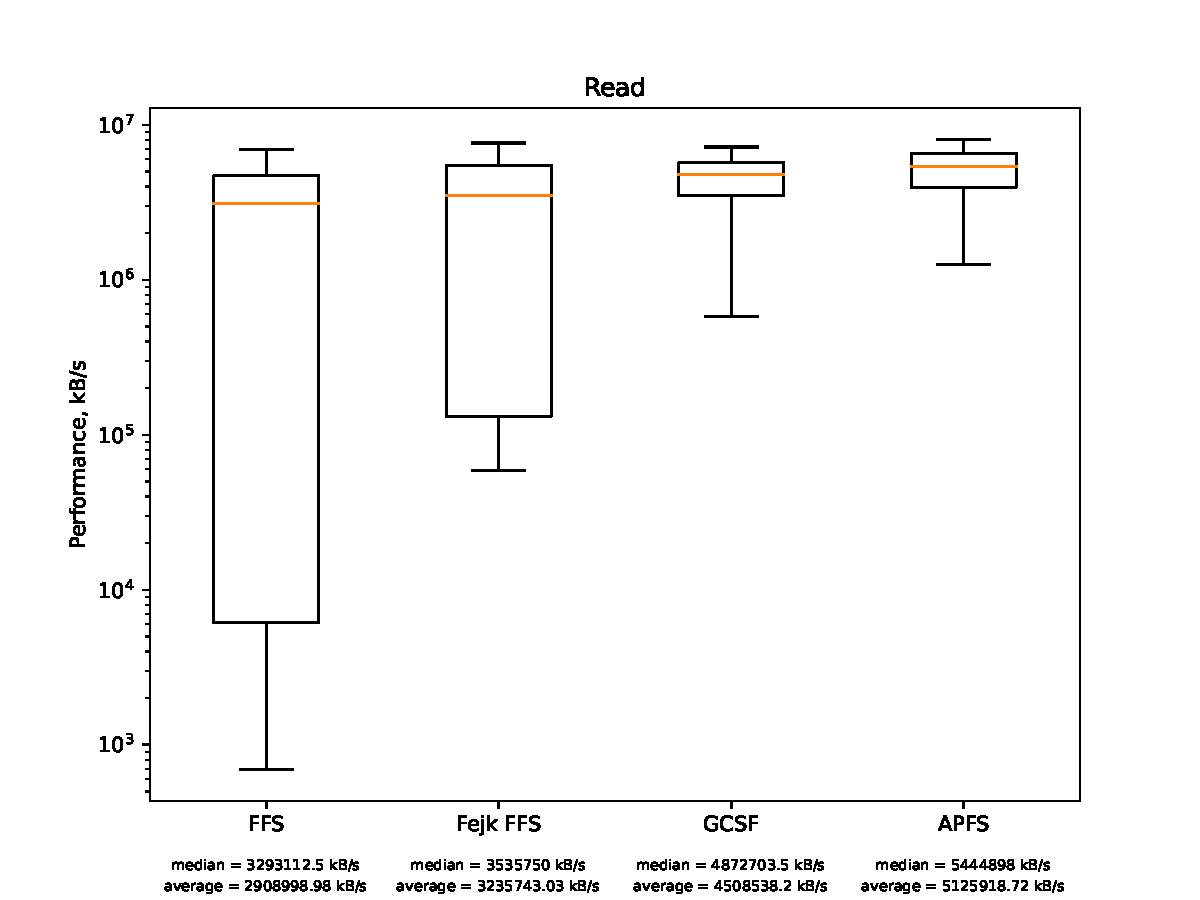
\includegraphics[width=1.0\textwidth]{figures/benchmarking/Read_box.pdf}
	\end{center}
	\caption{Box plot of the IOZone output for the Read test on the different filesystems}
\end{figure}

\FloatBarrier

Figure~\ref{fig:res_box_write} presents a box plot of the benchmarking results of the filesystems of the Write test. \gls{APFS} has the best write performance of the four filesystems, followed by \gls{FFFS}. The cloud-based filesystems \gls{FFS} and \gls{GCSF} have the worst median write performance, where \gls{FFS} has the worst performance of the filesystems. Comparing with the results of the Read test as presented in Figure~\ref{fig:res_box_read}, it can also be noted that the write performance is significantly worse for the write operations than the read operations for all filesystems. The average performance of the Write test for \gls{APFS} is 12.9\% of the Read performance. For \gls{FFFS}, \gls{GCSF}, and \gls{FFS} this percentage is 0.29\%, 0.17\%, and 0.06\%.

\begin{figure}[!ht]
	\label{fig:res_box_write}
	\begin{center}
		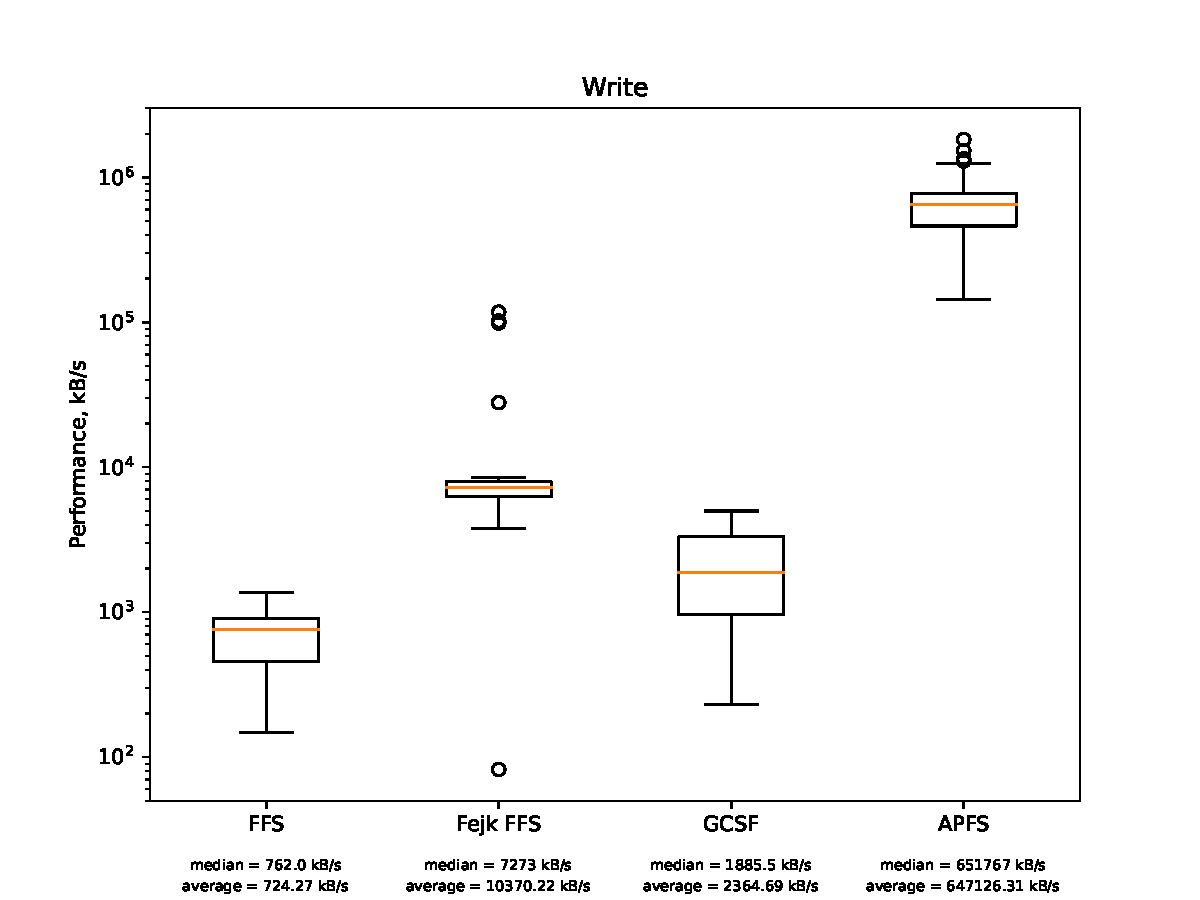
\includegraphics[width=1.0\textwidth]{figures/benchmarking/Write_box.pdf}
	\end{center}
	\caption{Box plot of the IOZone output for the Write test on the different filesystems}
\end{figure}

\FloatBarrier

Figure~\ref{fig:res_box_reread} presents the result of the \mbox{Re-Read} test for the filesystems. The median performance of the filesystems are similar, with the performance of \gls{FFS} being lowest. The spread of the values for \gls{APFS} is greater than for the other filesystems but the filesystem still has the best median and average performance. While the average performance for the Re-Read test of \gls{APFS} is around \SI[per-mode = symbol]{5.4}{\giga\byte\per\second}, the lowest performance was at \SI[per-mode = symbol]{422414}{\kilo\byte\per\second}, namely for \texttt{file size = 32768, buffer size = 8}. The spread of values is higher for \gls{FFS} than for \gls{FFFS} and \gls{GCSF}. \gls{FFFS} has a higher average and median performance than \gls{GCSF}.

\begin{figure}[!ht]
	\label{fig:res_box_reread}
	\begin{center}
		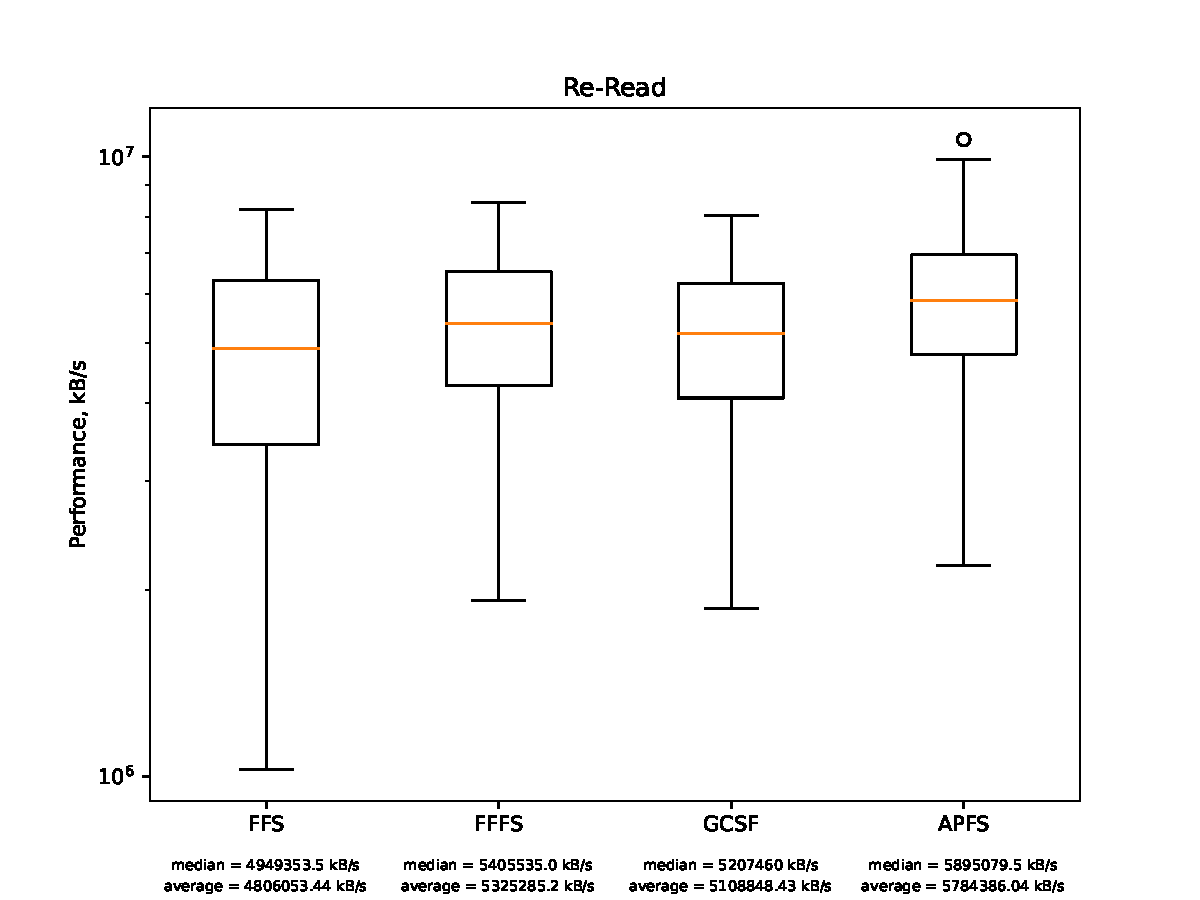
\includegraphics[width=1.0\textwidth]{figures/benchmarking/Re-Read_box.pdf}
	\end{center}
	\caption{Box plot of the IOZone output for the Re-Read test on the different filesystems}
\end{figure}

\FloatBarrier

Figure~\ref{fig:res_box_rewrite} presents a box plot for the \mbox{Re-Write} test for the filesystems. Similar to the Write test results presented in Figure~\ref{fig:res_box_write}, \gls{APFS} has the best performance of the filesystems, followed by \gls{FFFS} and finally the two cloud-based filesystems. \gls{APFS} is the only filesystem that has higher average and median performance for the \mbox{Re-Write} test compared to its Write test, with 22\% better median performance. The other filesystems has worse average and median performance for the \mbox{Re-Write} compared to their Write test. The median performance of the \mbox{Re-Write} test for \gls{FFS}, \gls{FFFS}, and \gls{GCSF} are 85\%, 82\%, and 64\% of the median performance of their Write test. 

\begin{figure}[!ht]
	\label{fig:res_box_rewrite}
	\begin{center}
		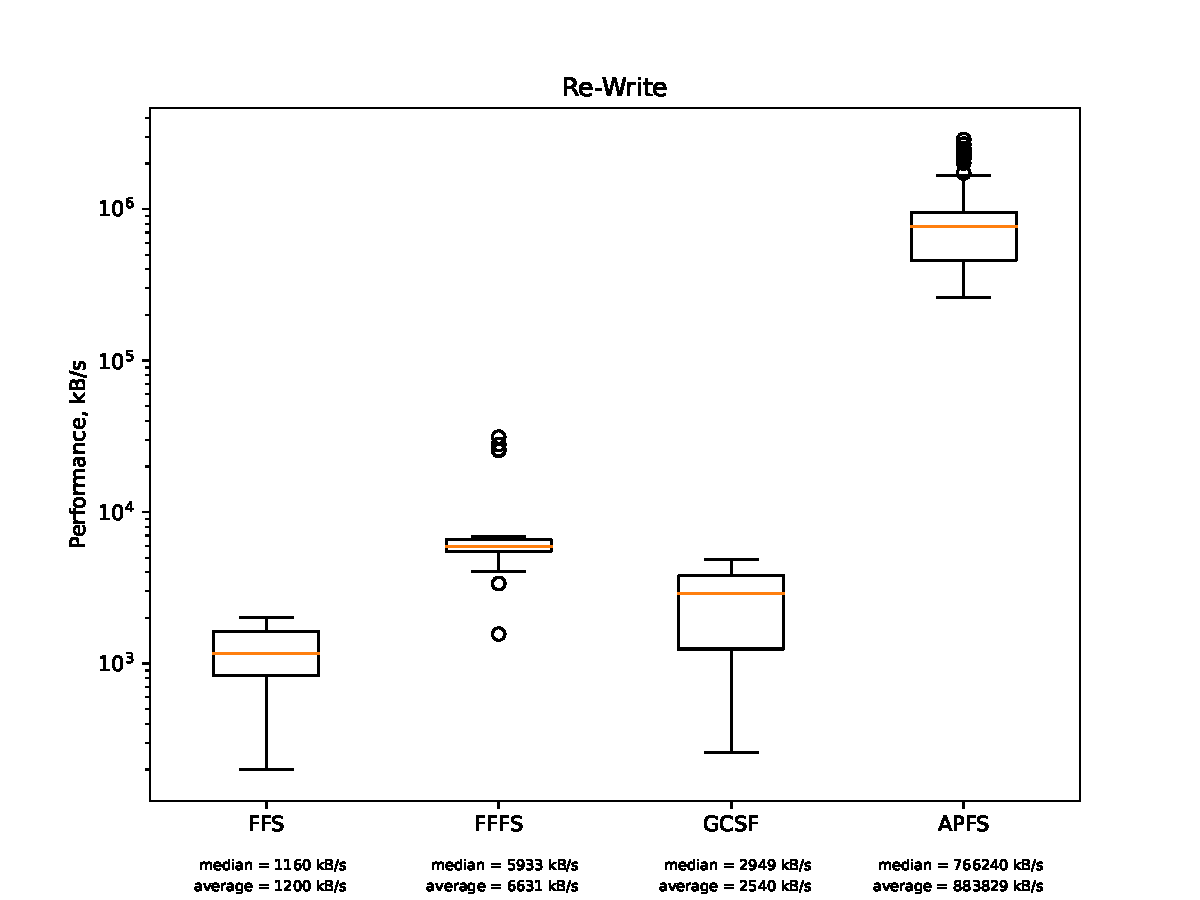
\includegraphics[width=1.0\textwidth]{figures/benchmarking/Re-Write_box.pdf}
	\end{center}
	\caption{Box plot of the IOZone output for the Re-Write test on the different filesystems}
\end{figure}

\FloatBarrier

Figure~\ref{fig:res_box_rndread} presents a box plot for the Random read test for the different filesystems. The results are similar to the results for the \mbox{Re-Read} test presented in Figure~\ref{fig:res_box_reread}, however, \gls{FFS} has bigger spread of values than \gls{APFS} has in the \mbox{Re-Read} test. \gls{FFFS} has the best average performance of the filesystems, and \gls{APFS} has the best median performance. The median and average performance of \gls{FFS} is lower than the other filesystems.

\begin{figure}[!ht]
	\label{fig:res_box_rndread}
	\begin{center}
		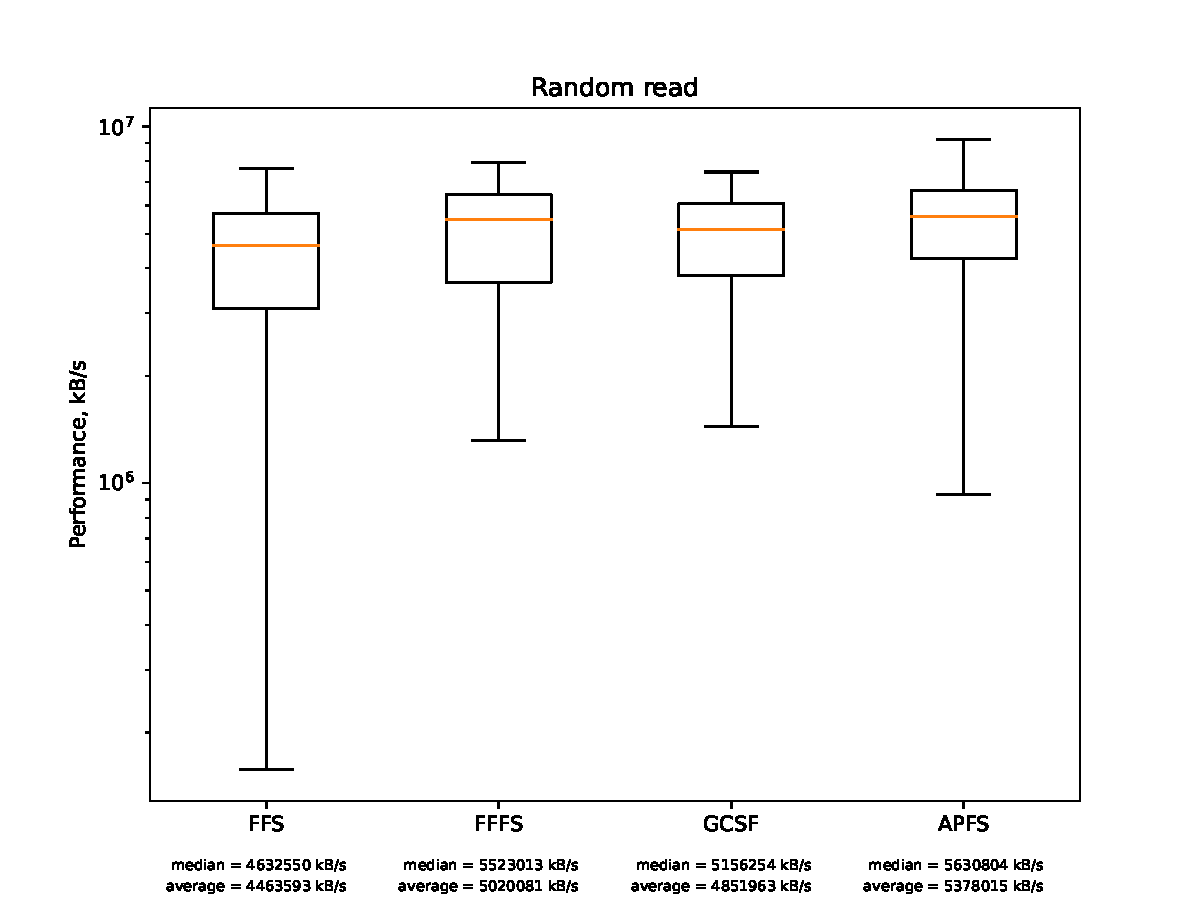
\includegraphics[width=1.0\textwidth]{figures/benchmarking/Random read_box.pdf}
	\end{center}
	\caption{Box plot of the IOZone output for the Random read test on the different filesystems}
\end{figure}

\FloatBarrier

Figure~\ref{fig:res_box_rndwrite} presents a box plot for the Random read test for the different filesystems. \gls{APFS} has the highest performance, followed by \gls{FFFS} and the cloud-based filesystems. \gls{GCSF} has better performance than \gls{FFS}. The performances are similar to the \mbox{Re-Write} for all filesystems.

\begin{figure}[!ht]
	\label{fig:res_box_rndwrite}
	\begin{center}
		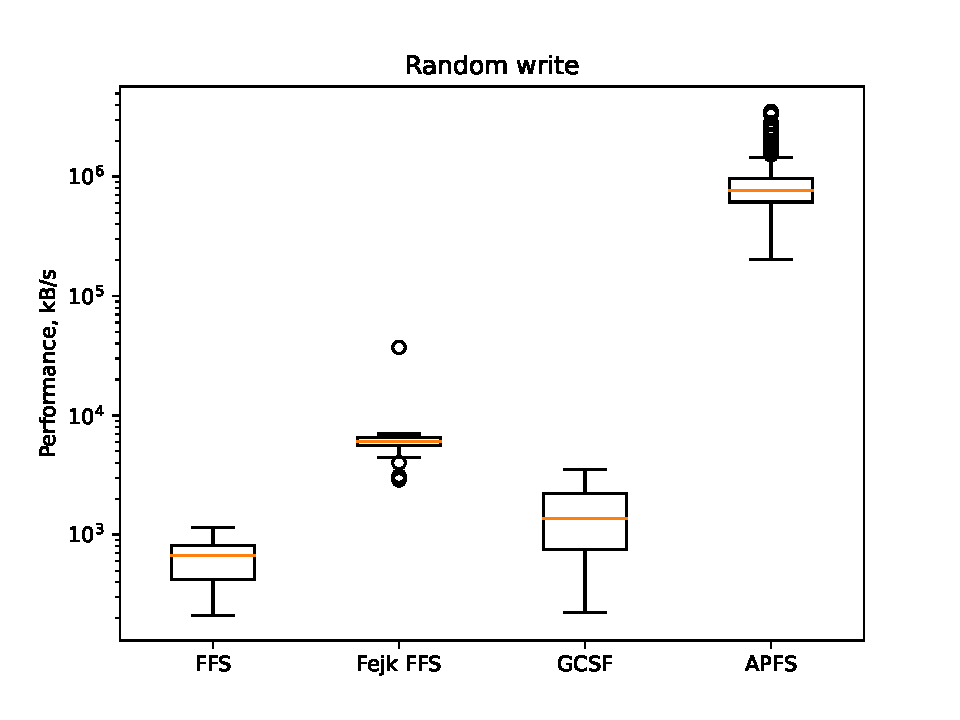
\includegraphics[width=1.0\textwidth]{figures/benchmarking/Random write_box.pdf}
	\end{center}
	\caption{Box plot of the IOZone output for the Random write test on the different filesystems}
\end{figure}

\FloatBarrier

\gls{FFS} does not have the best performance in any of the box plots presented. \gls{GCSF} has better performance than \gls{FFS} for all tests run with the benchmarking. Following are diagrams presenting the performance of each benchmarking test per file size, for each filesystem. The raw data tables can be found in Appendix~\ref{app:bench_data}. Figure~\ref{fig:bench_ffs_read}, Figure~\ref{fig:bench_ffs_write}, Figure~\ref{fig:bench_ffs_re_read}, Figure~\ref{fig:bench_ffs_re_write}, Figure~\ref{fig:bench_ffs_rnd_read}, and Figure~\ref{fig:bench_ffs_rnd_write} presents the performances of the Read, Write, \mbox{Re-Read}, \mbox{Re-Write}, Random Read, and Random Write tests for \gls{FFS}.

\begin{figure}[!htb]
	\label{fig:bench_ffs_read}
	\begin{center}
		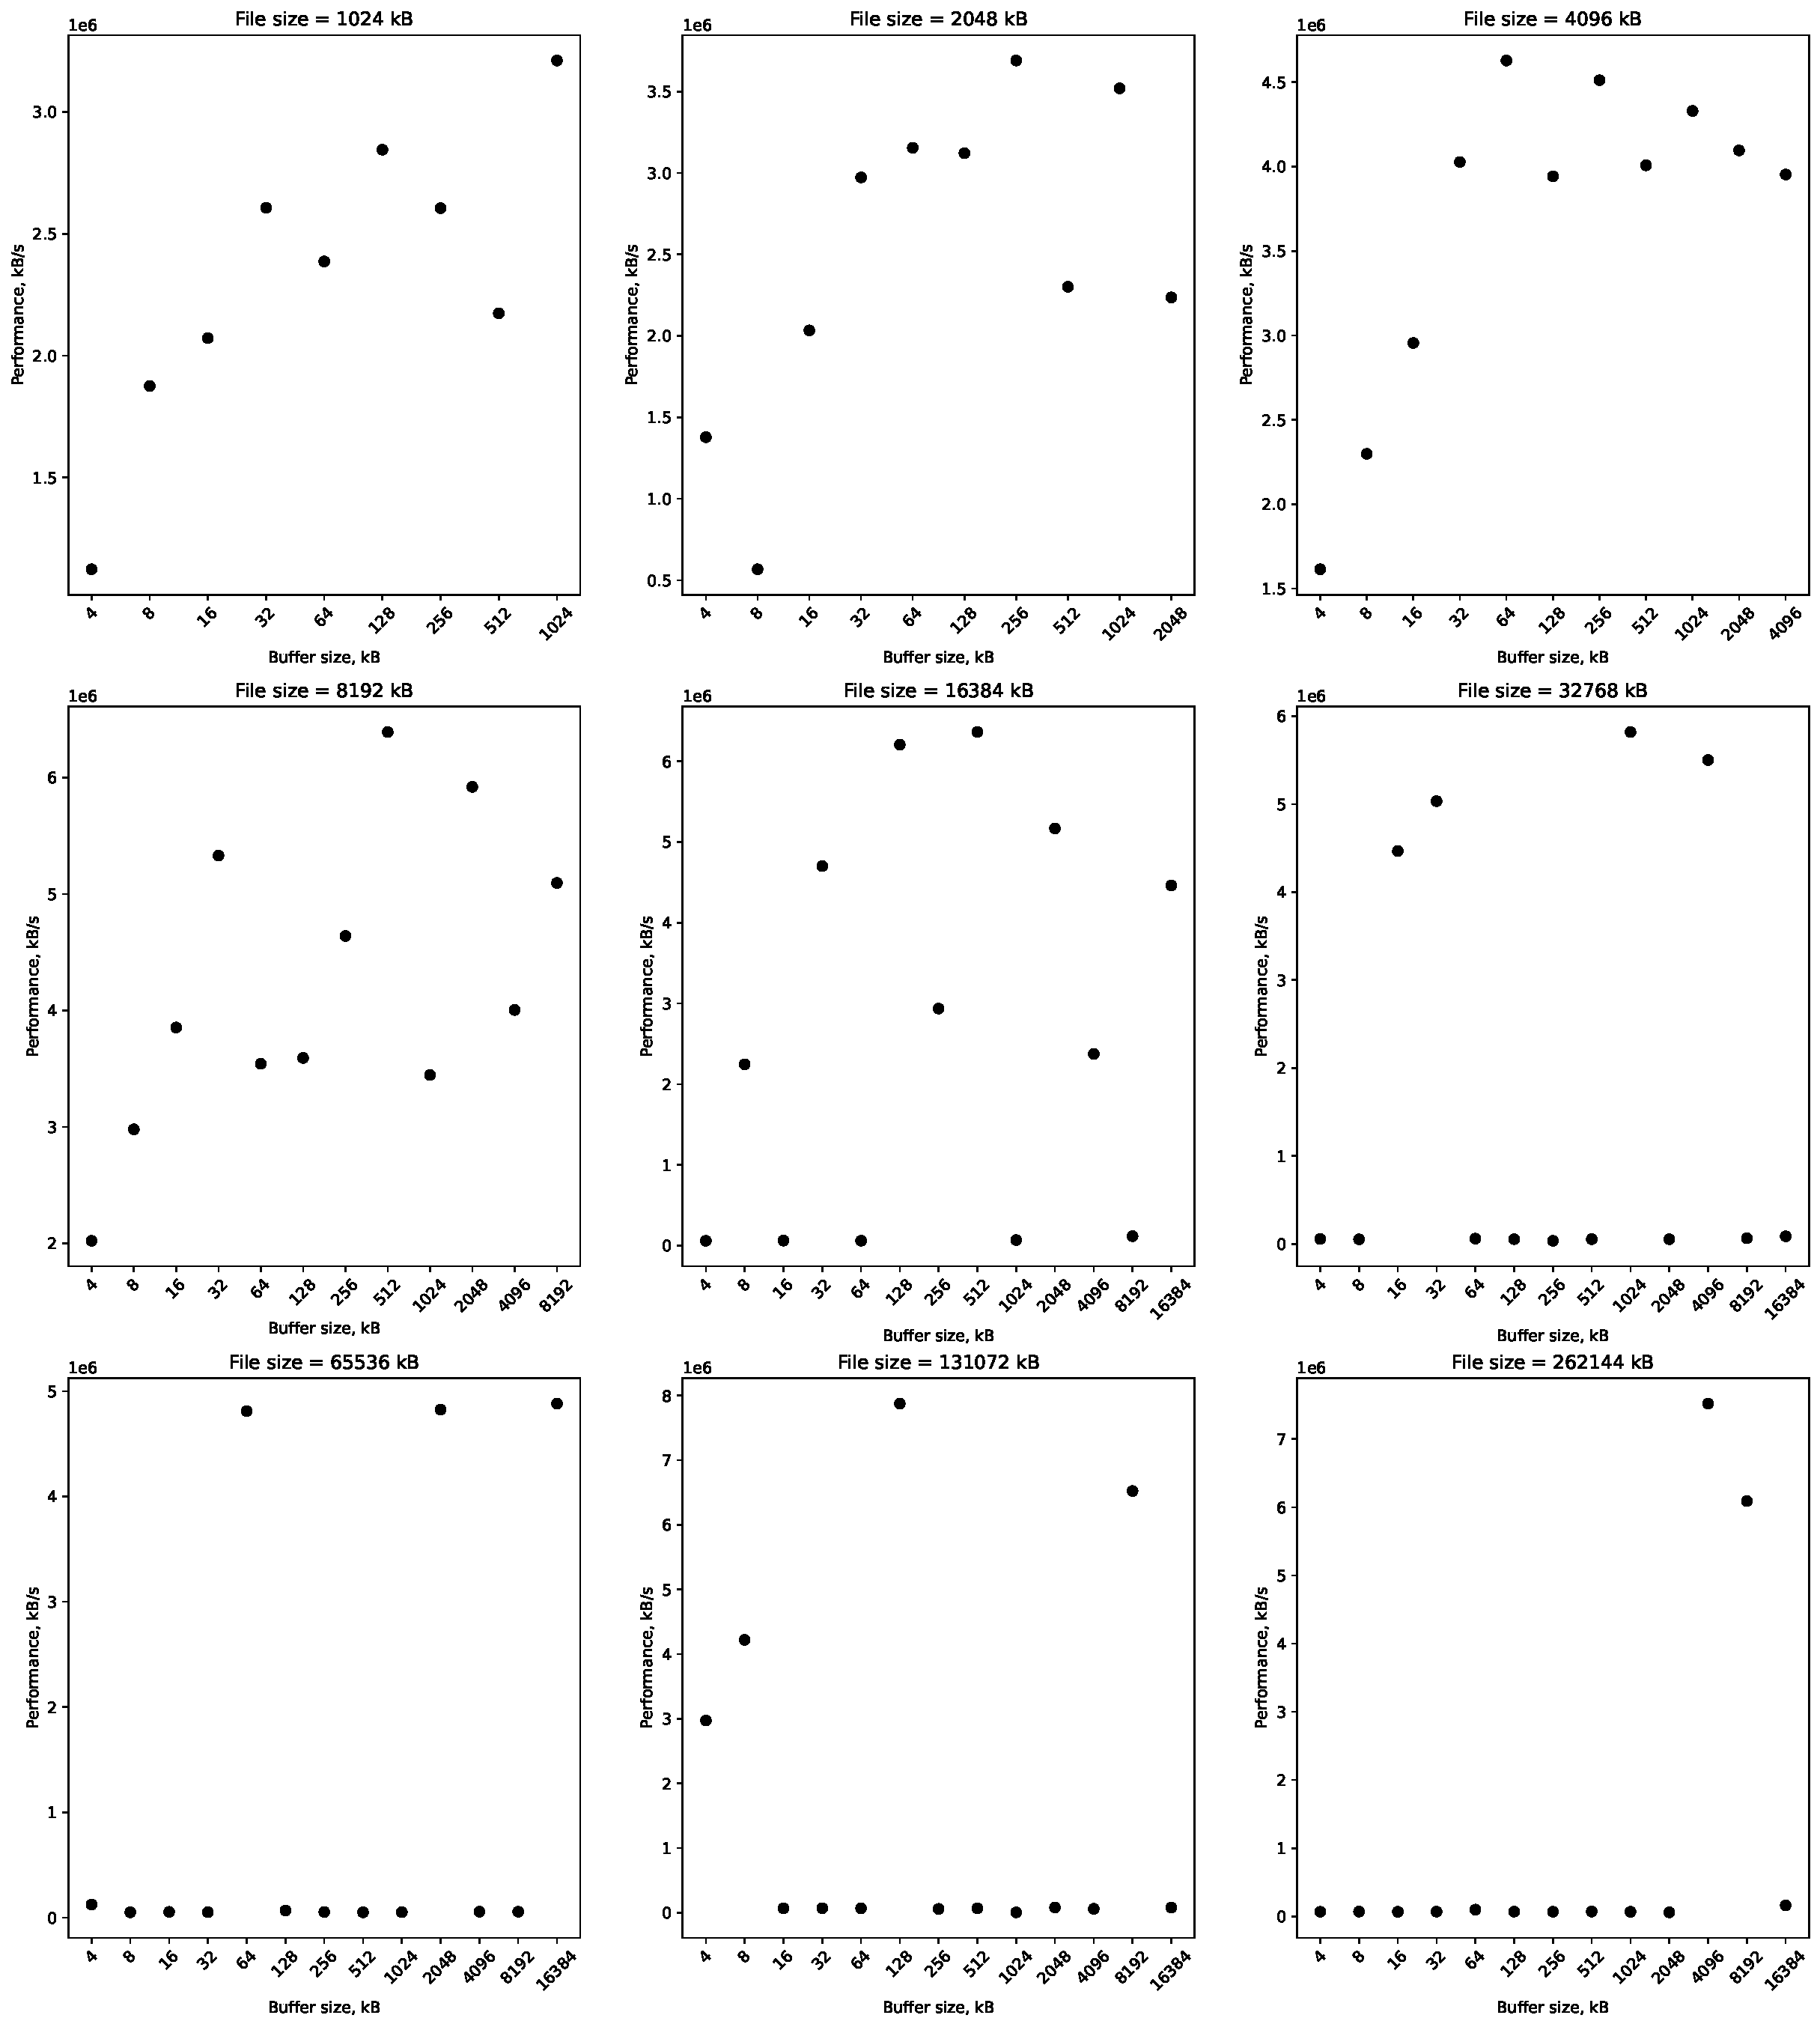
\includegraphics[width=1.0\textwidth]{figures/benchmarking/ffs/Read.pdf}
	\end{center}
	\caption{IOZone output for FFS Read}
\end{figure}

\begin{figure}[!htb]
	\label{fig:bench_ffs_write}
	\begin{center}
		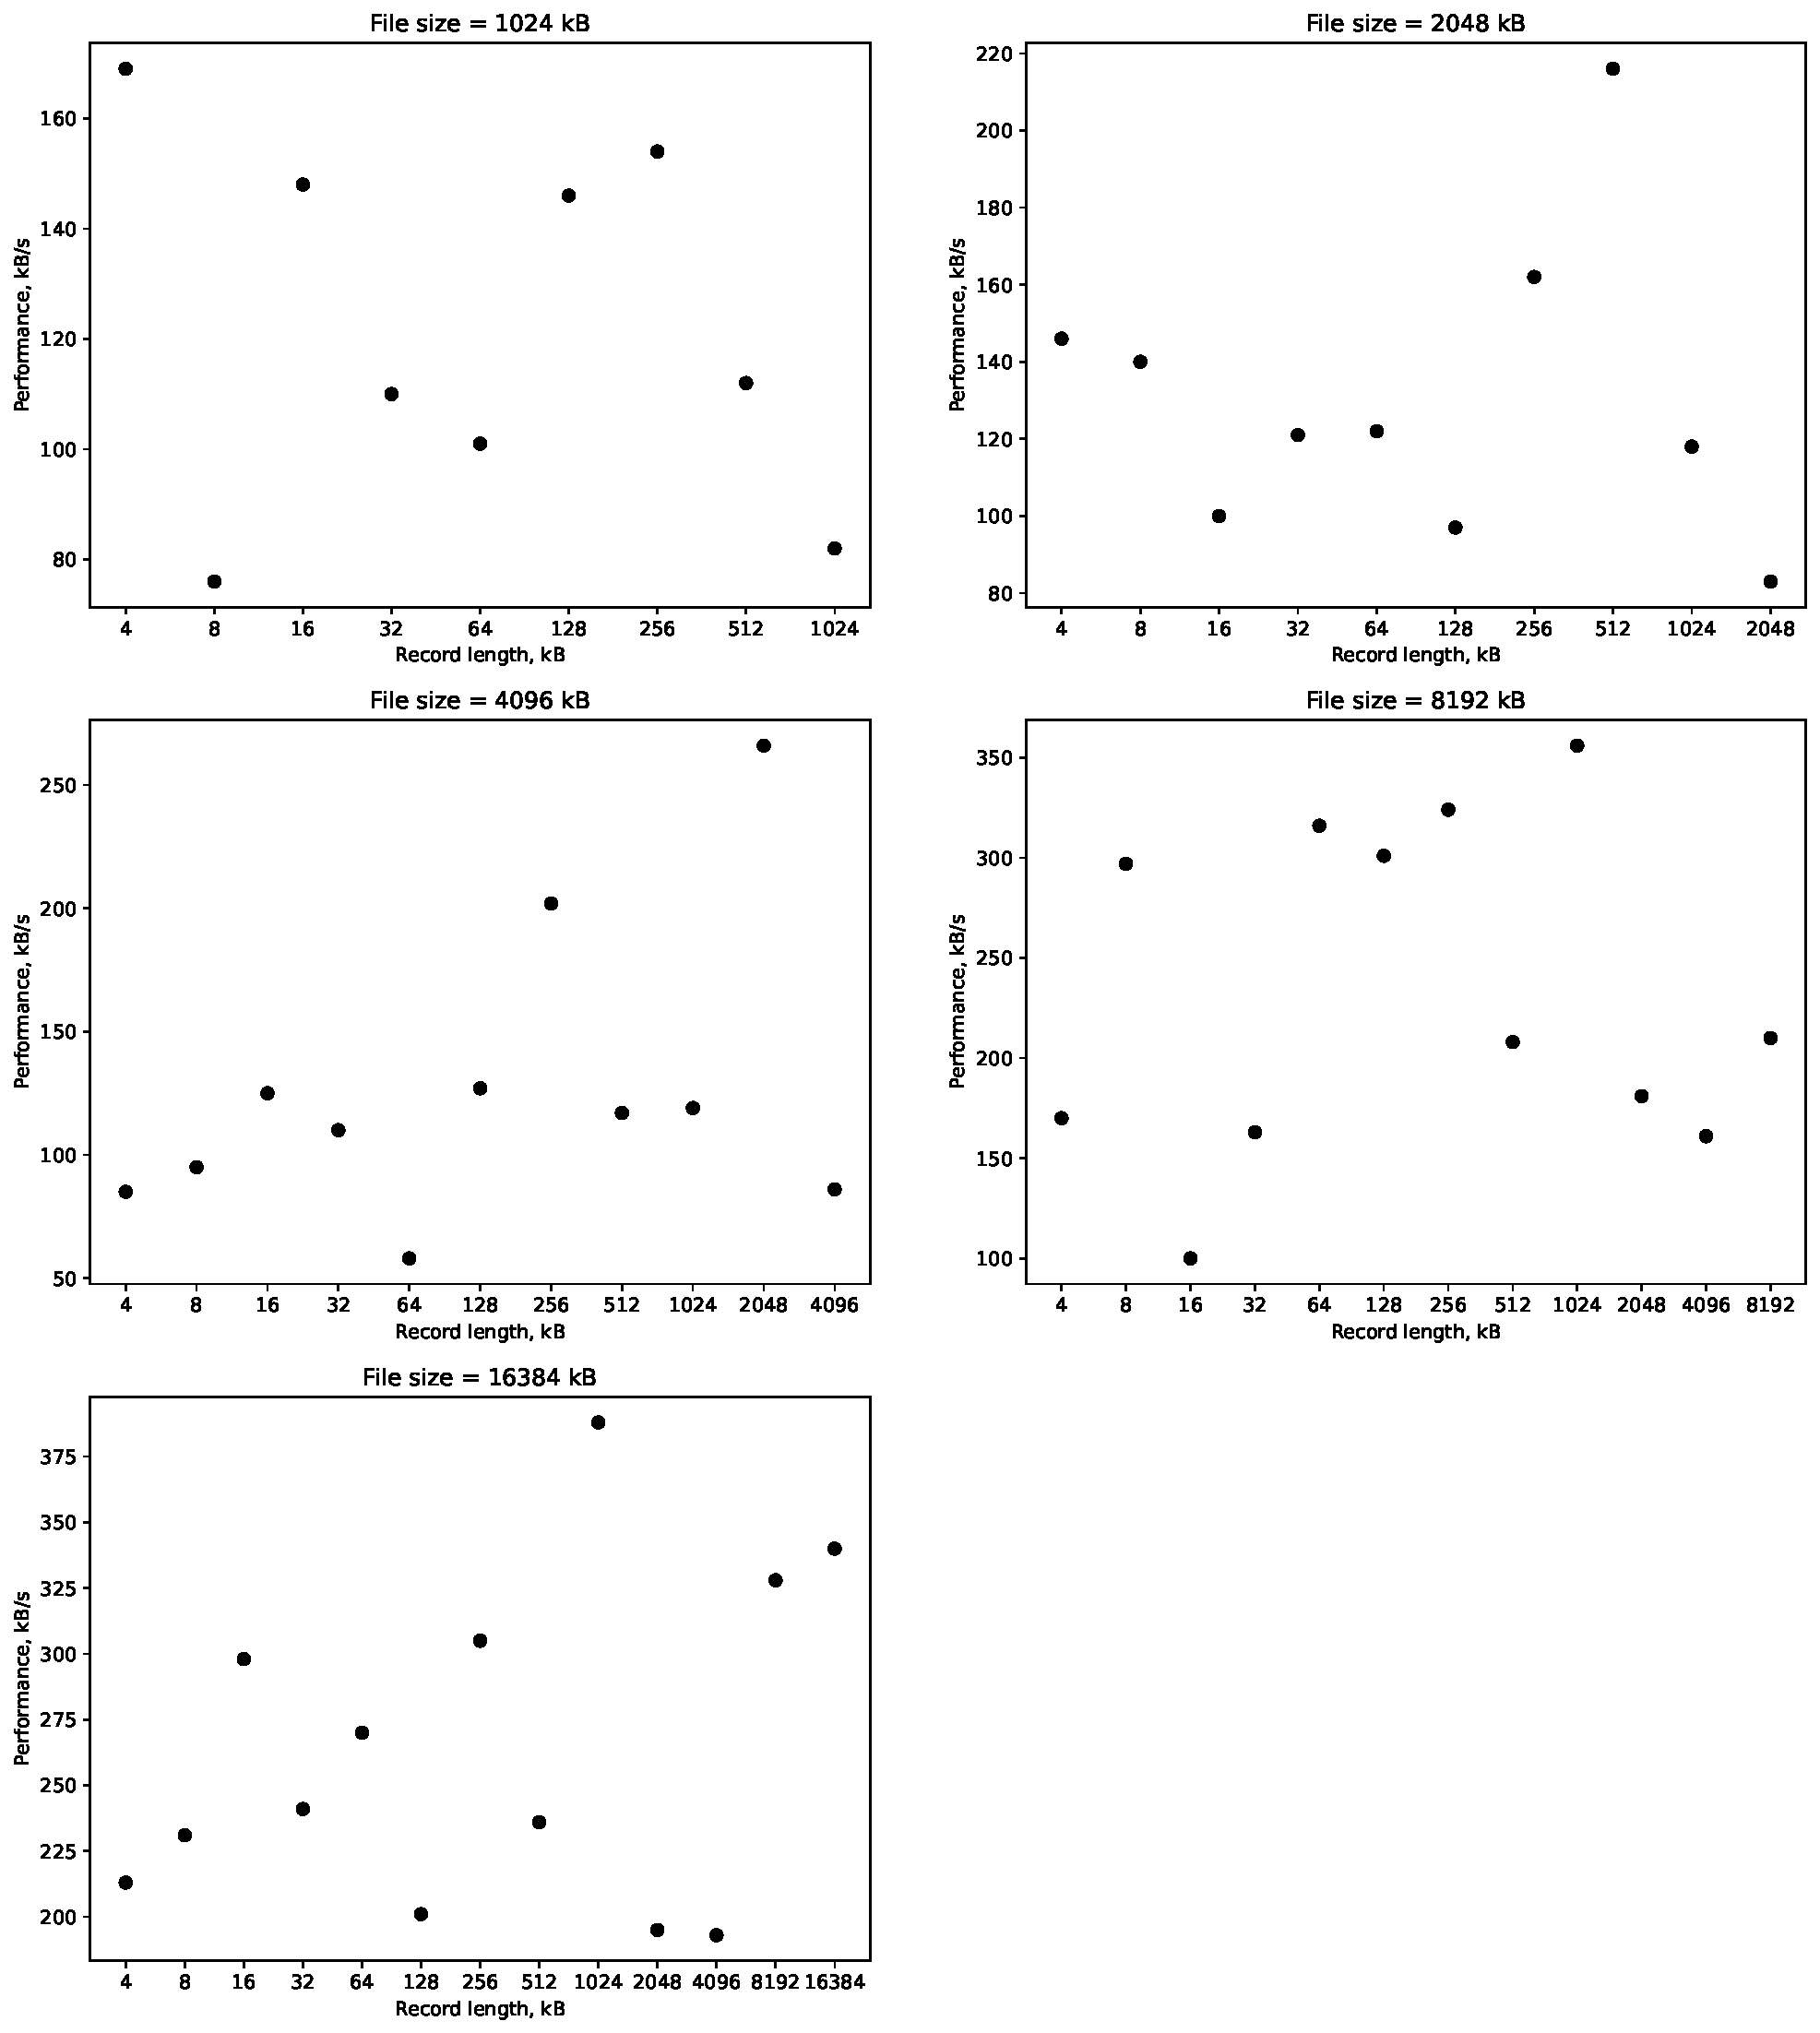
\includegraphics[width=1.0\textwidth]{figures/benchmarking/ffs/Write.pdf}
	\end{center}
	\caption{IOZone output for FFS Write}
\end{figure}

\begin{figure}[!htb]
	\label{fig:bench_ffs_re_read}
	\begin{center}
		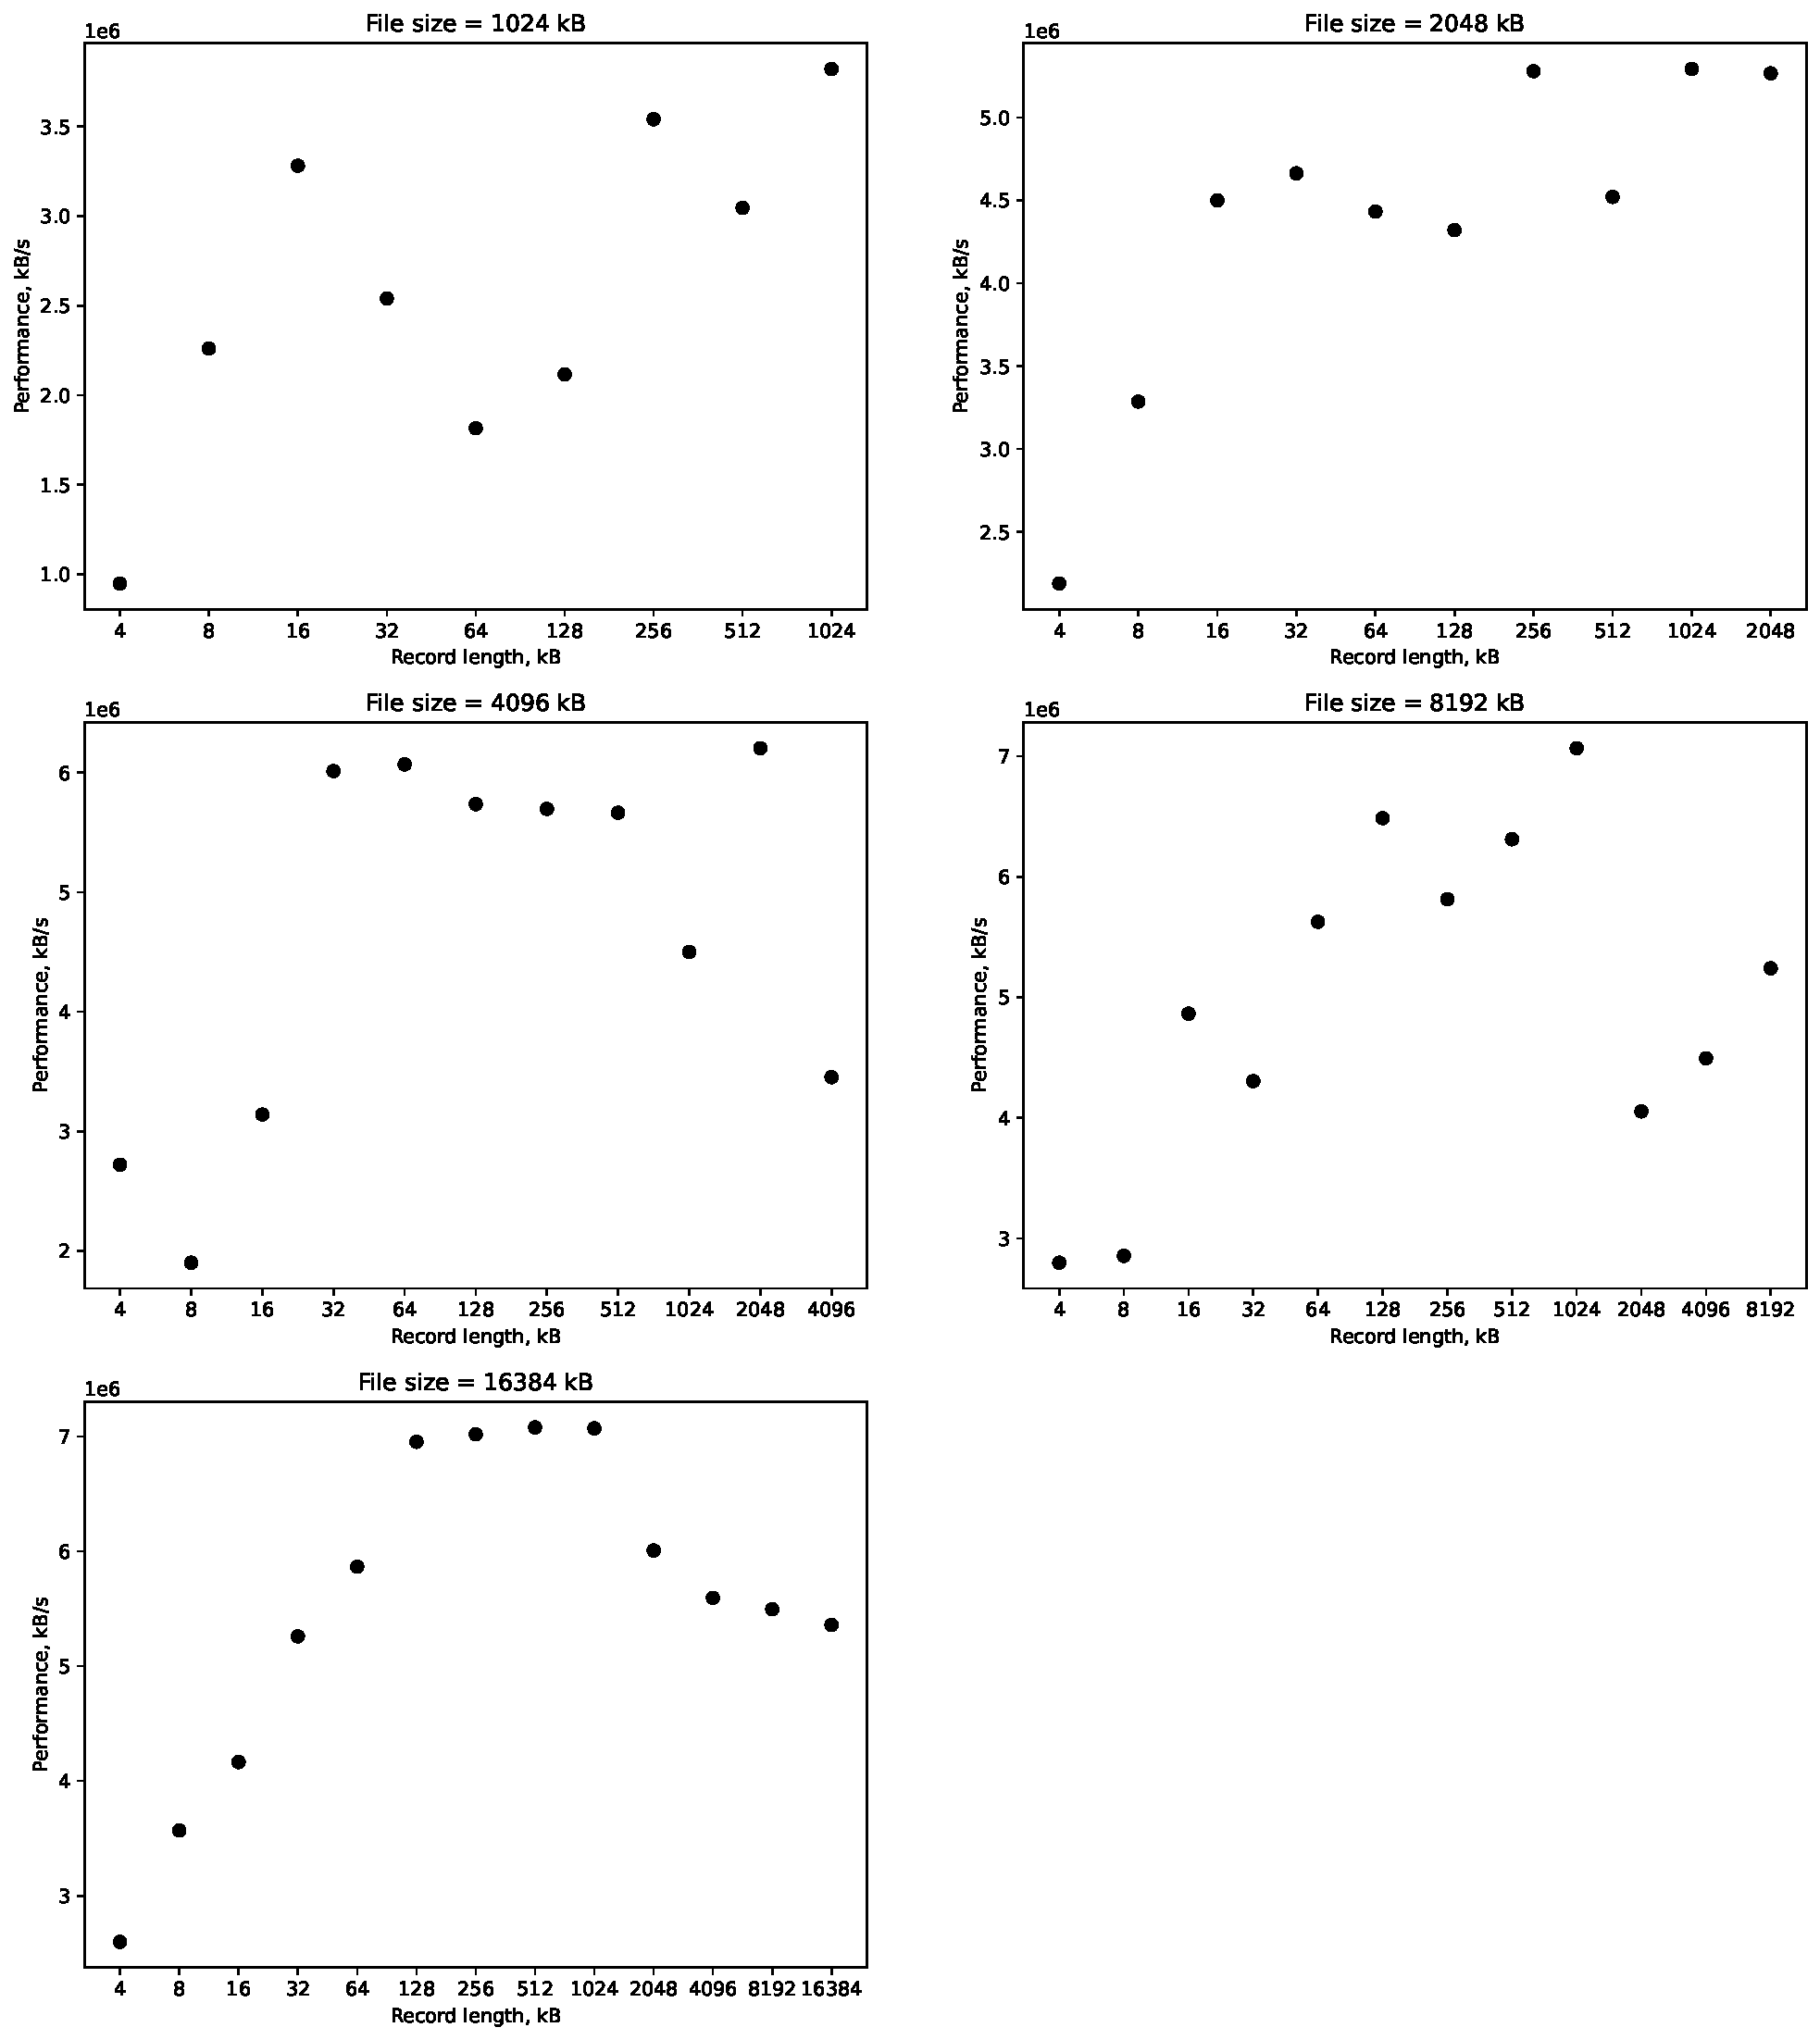
\includegraphics[width=1.0\textwidth]{figures/benchmarking/ffs/Re-Read.pdf}
	\end{center}
	\caption{IOZone output for FFS \mbox{Re-Read}}
\end{figure}

\begin{figure}[!htb]
	\label{fig:bench_ffs_re_write}
	\begin{center}
		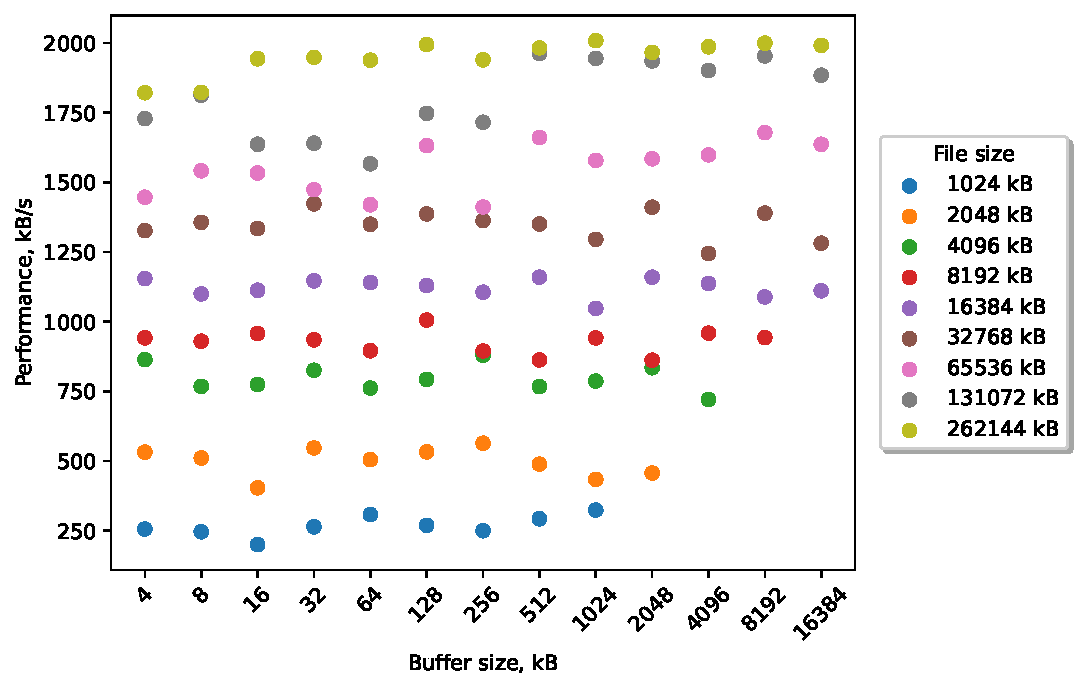
\includegraphics[width=1.0\textwidth]{figures/benchmarking/ffs/Re-Write.pdf}
	\end{center}
	\caption{IOZone output for FFS \mbox{Re-Write}}
\end{figure}

\begin{figure}[!htb]
	\label{fig:bench_ffs_rnd_read}
	\begin{center}
		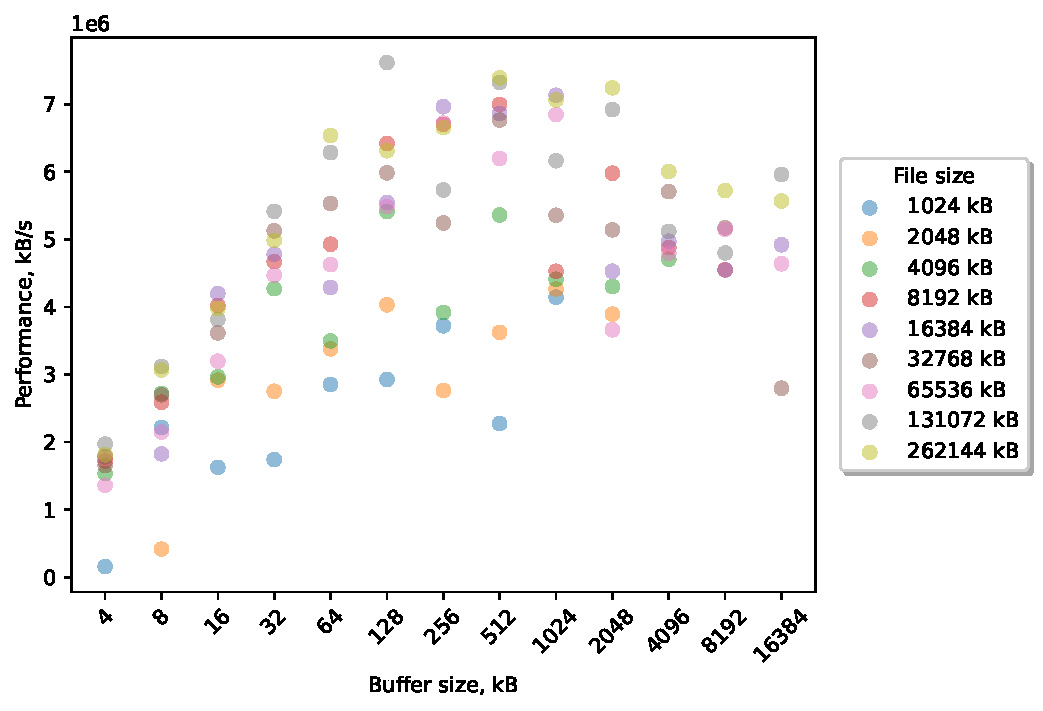
\includegraphics[width=1.0\textwidth]{figures/benchmarking/ffs/Random read.pdf}
	\end{center}
	\caption{IOZone output for FFS Random read}
\end{figure}

\begin{figure}[!htb]
	\label{fig:bench_ffs_rnd_write}
	\begin{center}
		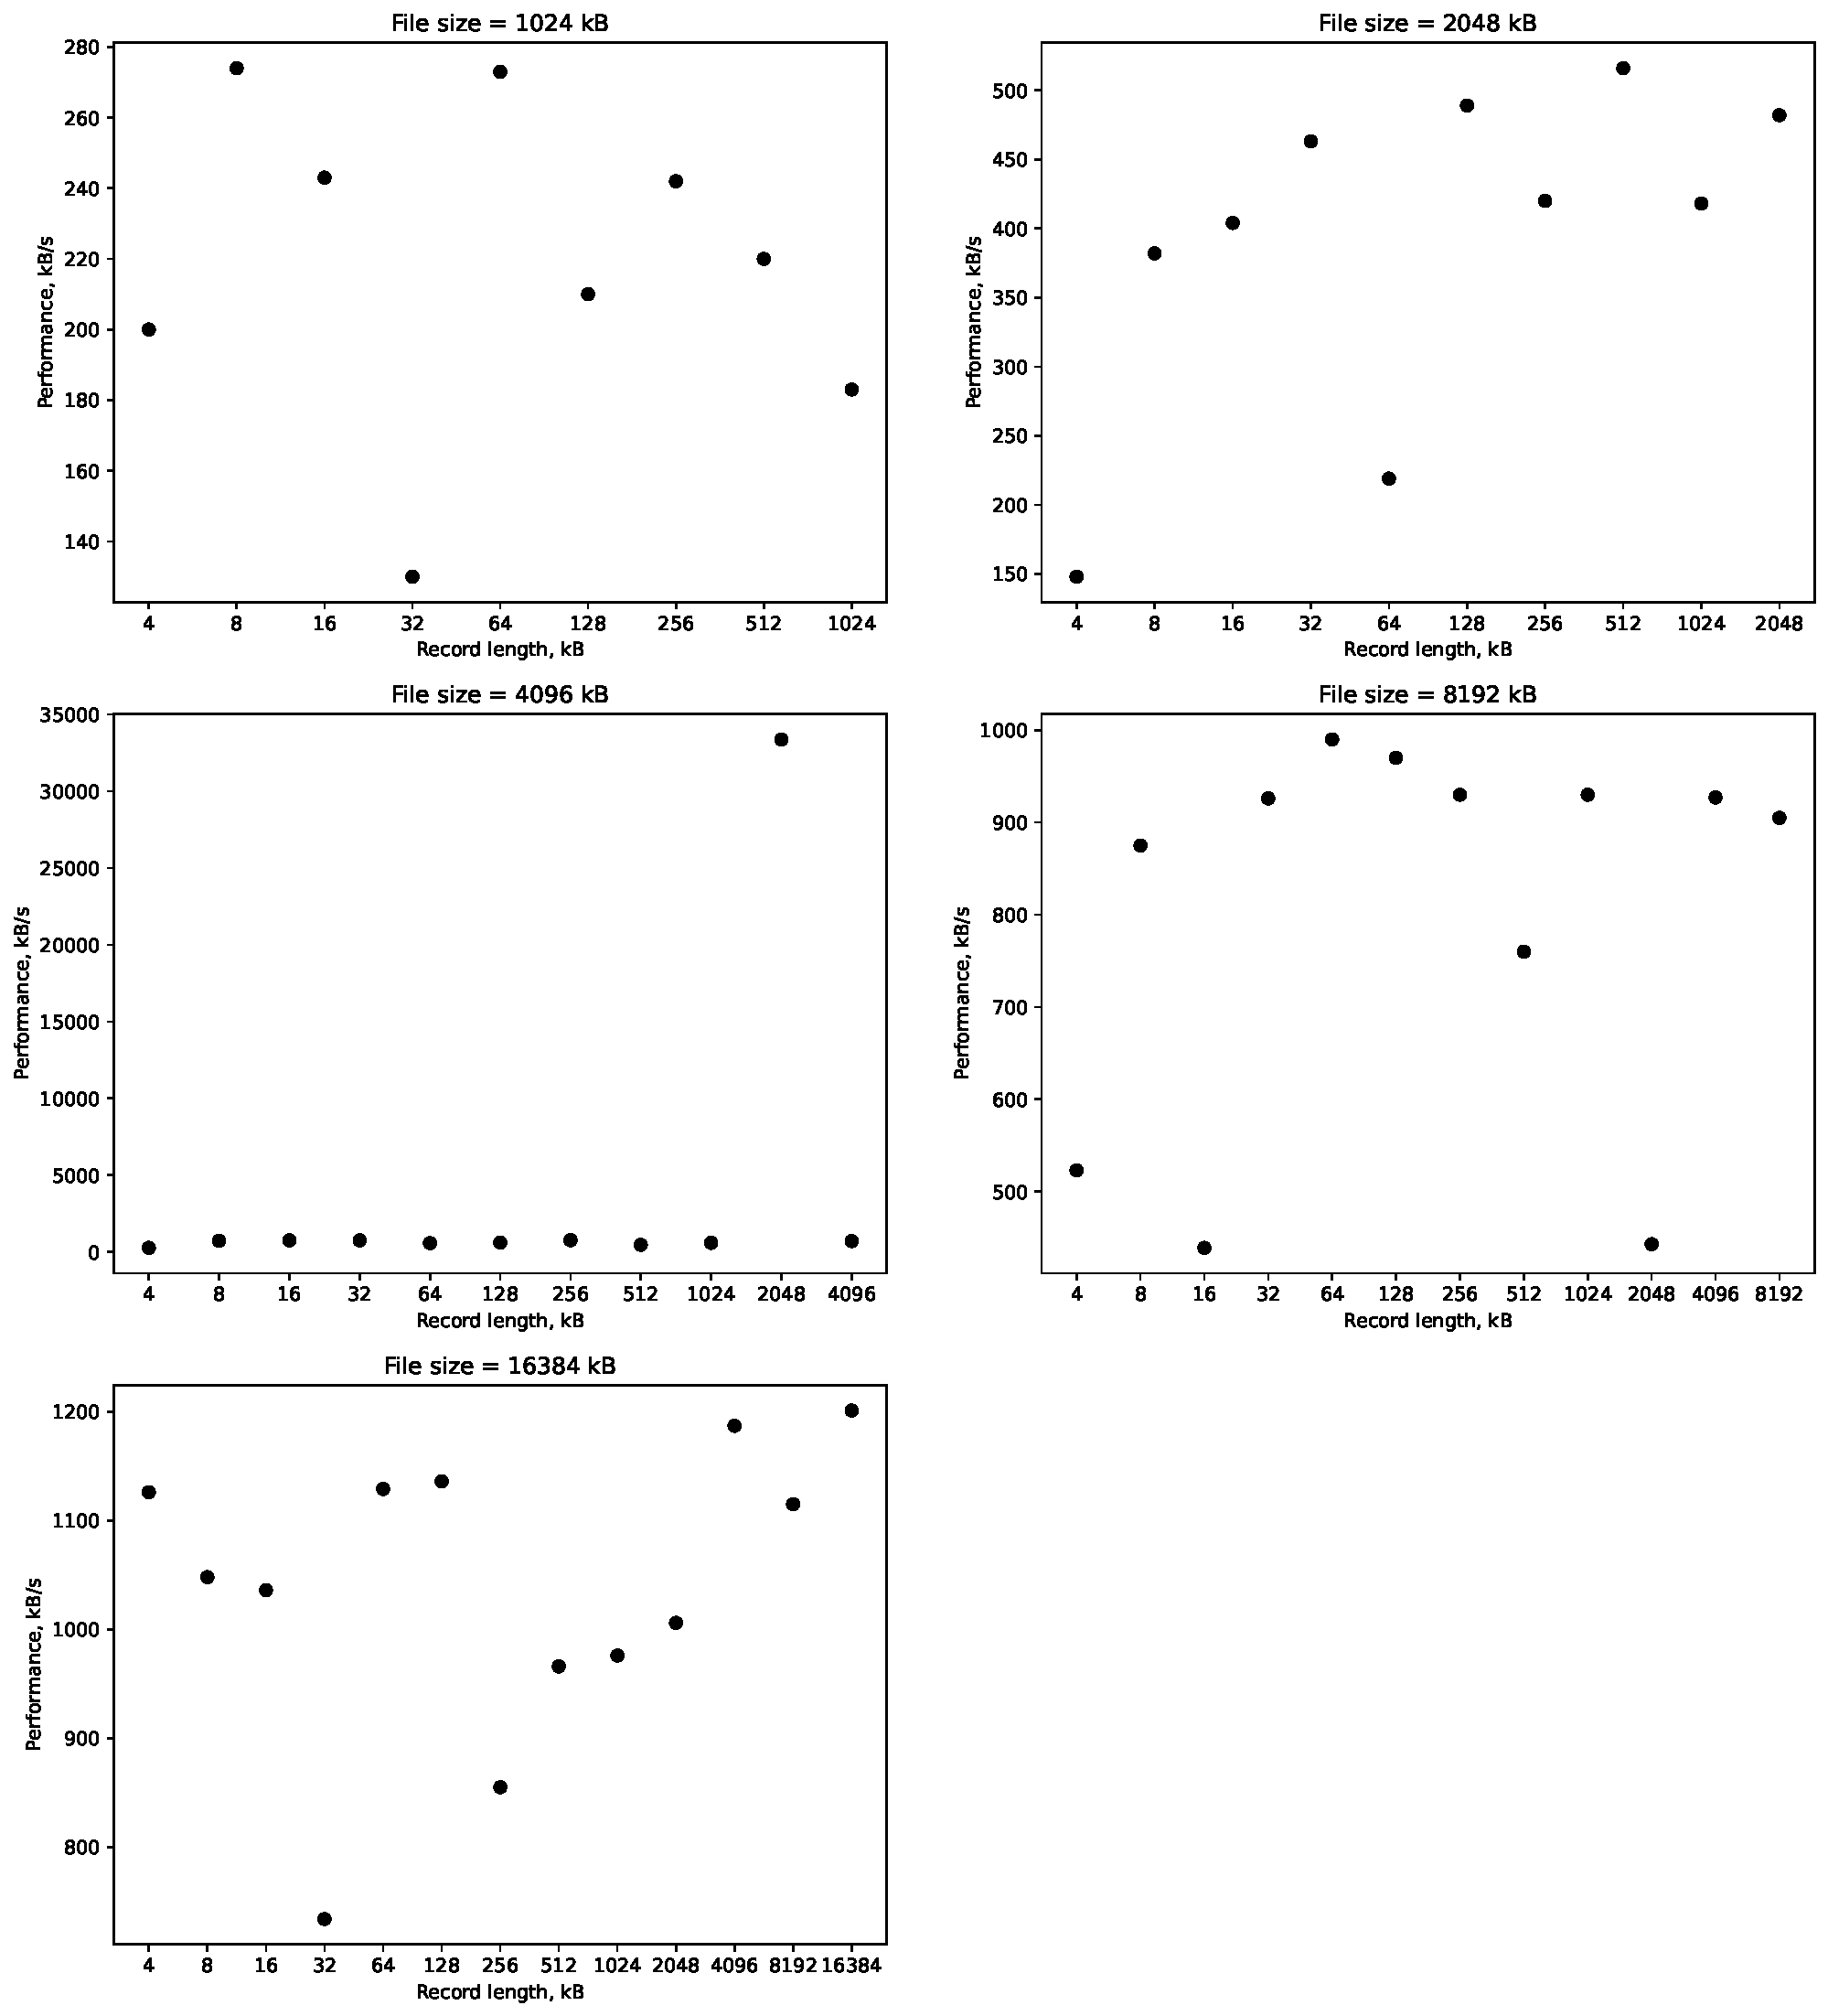
\includegraphics[width=1.0\textwidth]{figures/benchmarking/ffs/Random write.pdf}
	\end{center}
	\caption{IOZone output for FFS Random write}
\end{figure}

\FloatBarrier

Figure~\ref{fig:bench_fffs_read}, Figure~\ref{fig:bench_fffs_write}, Figure~\ref{fig:bench_fffs_re_read}, Figure~\ref{fig:bench_fffs_re_write}, Figure~\ref{fig:bench_fffs_rnd_read}, and Figure~\ref{fig:bench_fffs_rnd_write} presents the performances of the Read, Write, \mbox{Re-Read}, \mbox{Re-Write}, Random Read, and Random Write tests for \gls{FFFS}.

\begin{figure}[!htb]
	\label{fig:bench_fffs_read}
	\begin{center}
		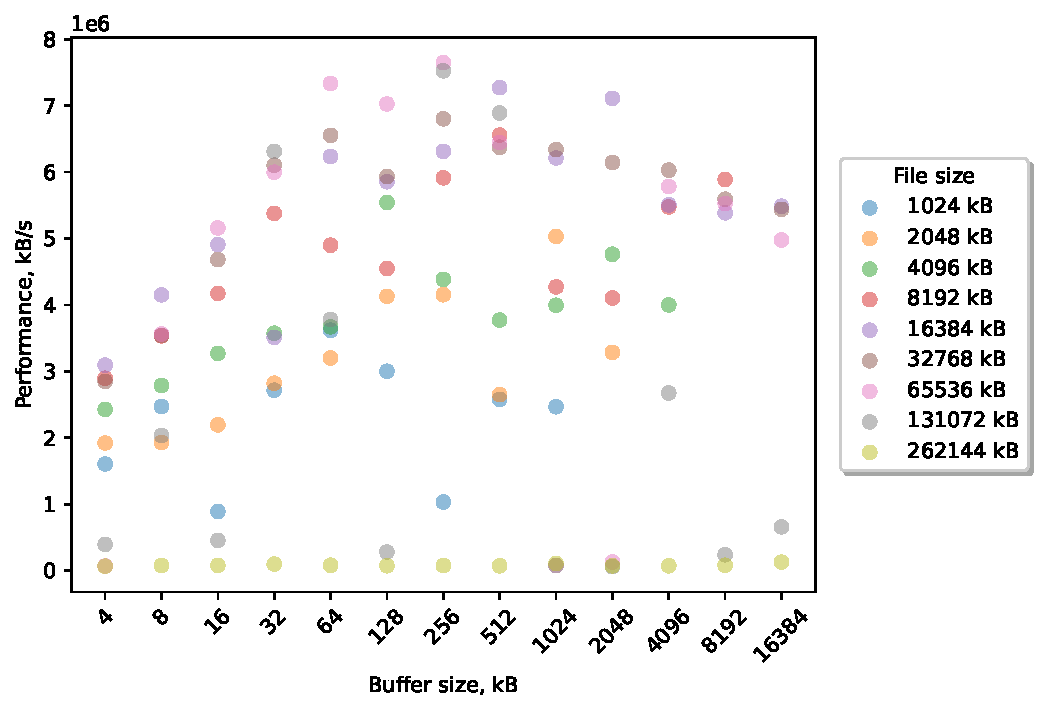
\includegraphics[width=1.0\textwidth]{figures/benchmarking/fejk-ffs/Read.pdf}
	\end{center}
	\caption{IOZone output for Fejk FFS Read}
\end{figure}

\begin{figure}[!htb]
	\label{fig:bench_fffs_write}
	\begin{center}
		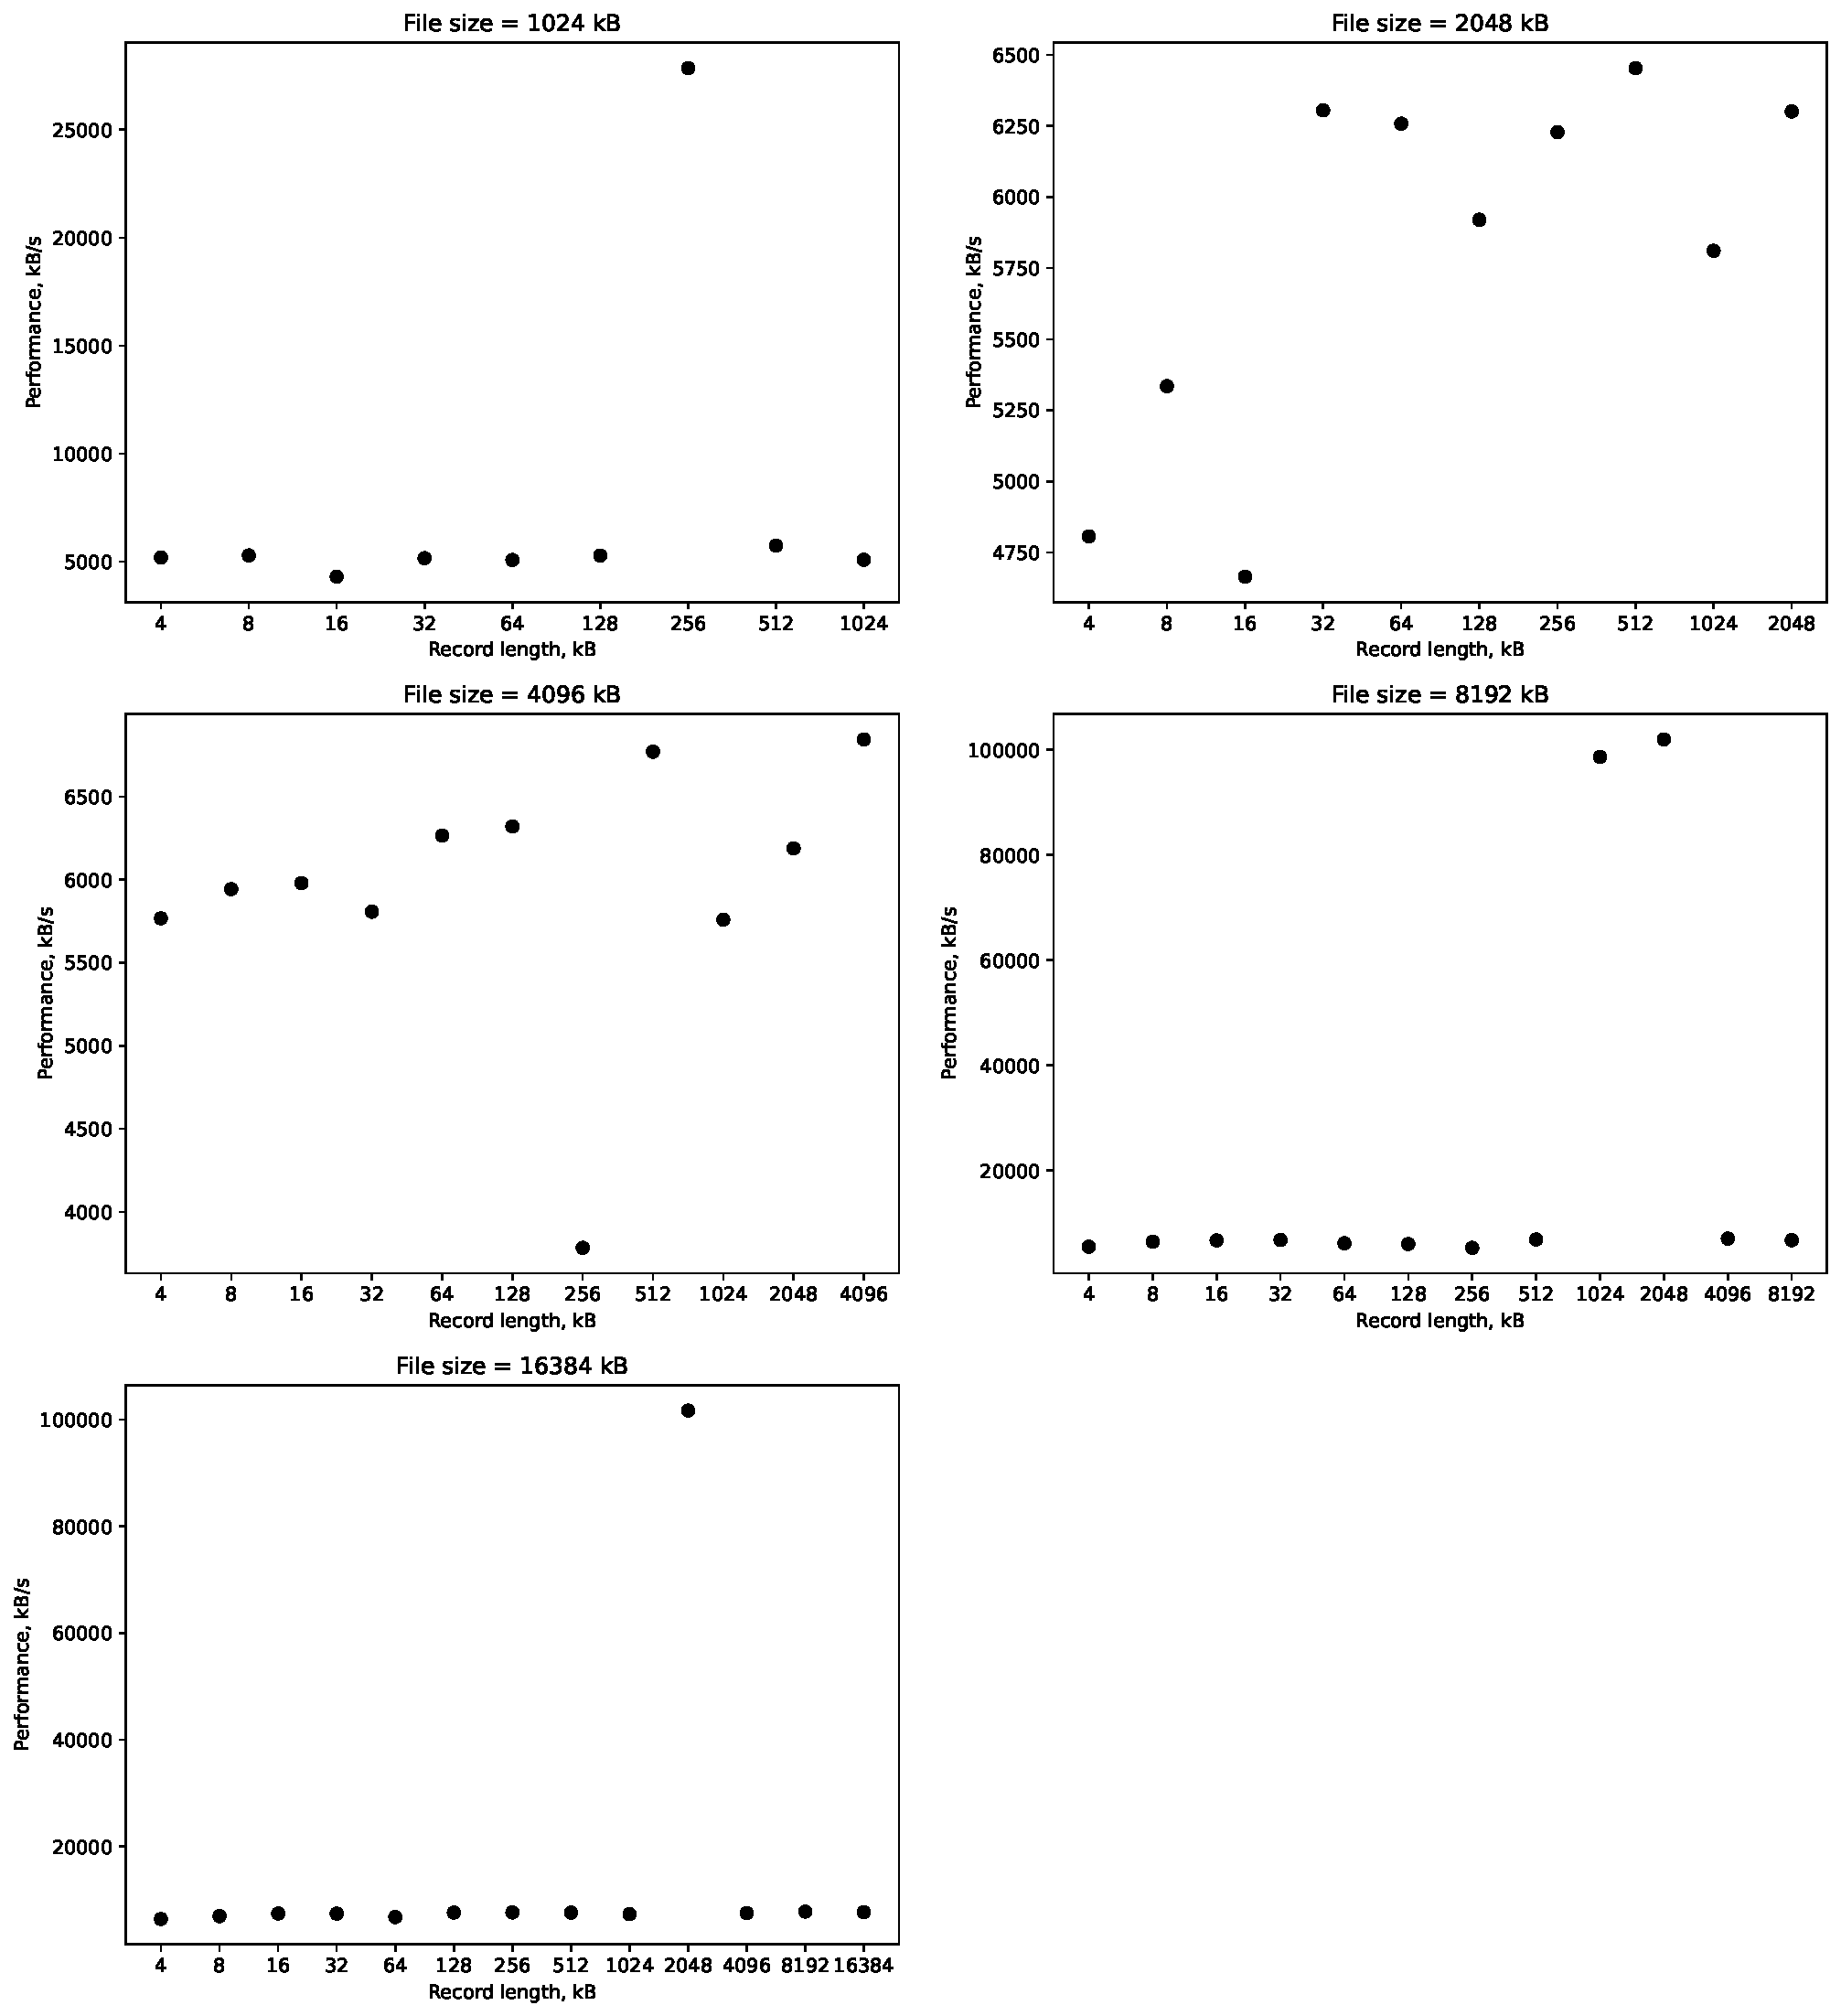
\includegraphics[width=1.0\textwidth]{figures/benchmarking/fejk-ffs/Write.pdf}
	\end{center}
	\caption{IOZone output for Fejk FFS Write}
\end{figure}

\begin{figure}[!htb]
	\label{fig:bench_fffs_re_read}
	\begin{center}
		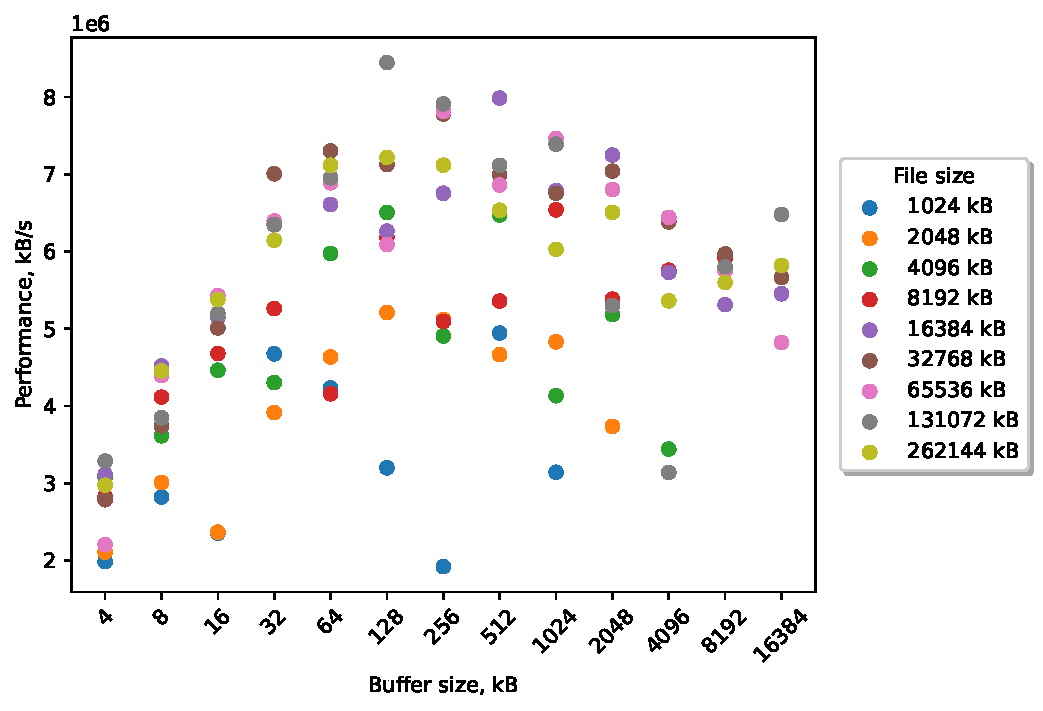
\includegraphics[width=1.0\textwidth]{figures/benchmarking/fejk-ffs/Re-Read.pdf}
	\end{center}
	\caption{IOZone output for Fejk FFS \mbox{Re-Read}}
\end{figure}

\begin{figure}[!htb]
	\label{fig:bench_fffs_re_write}
	\begin{center}
		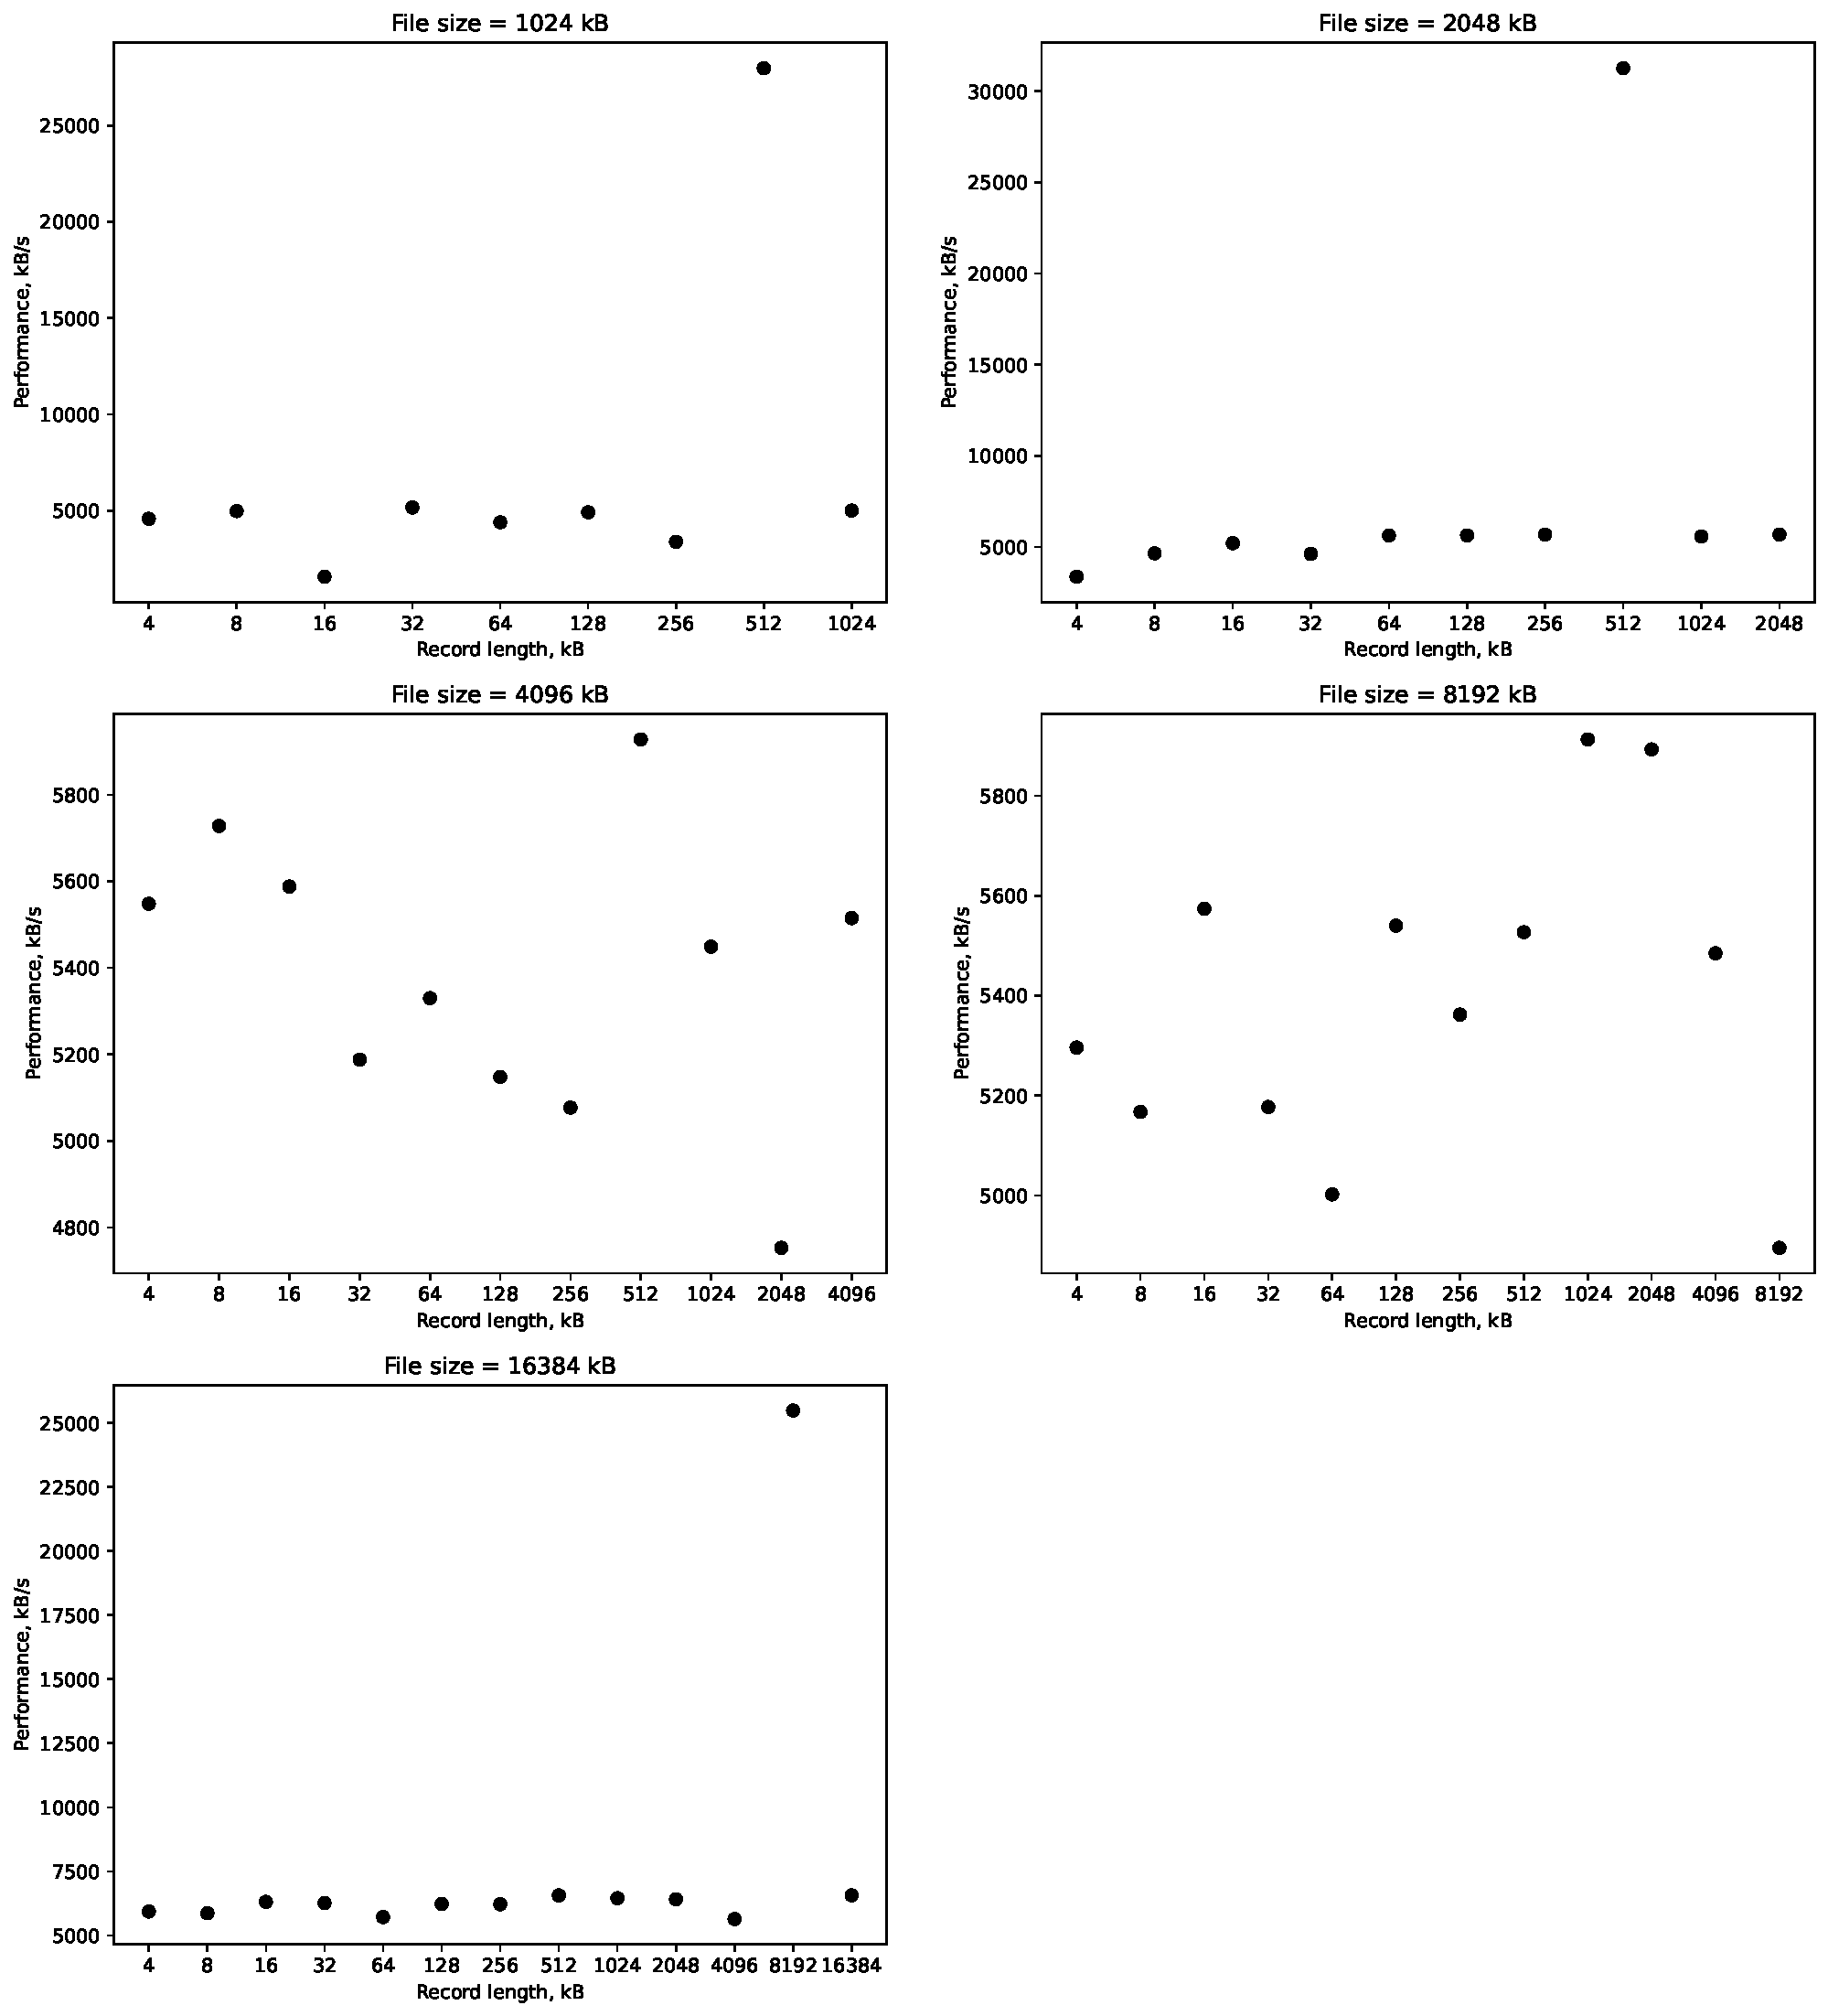
\includegraphics[width=1.0\textwidth]{figures/benchmarking/fejk-ffs/Re-Write.pdf}
	\end{center}
	\caption{IOZone output for Fejk FFS \mbox{Re-Write}}
\end{figure}

\begin{figure}[!htb]
	\label{fig:bench_fffs_rnd_read}
	\begin{center}
		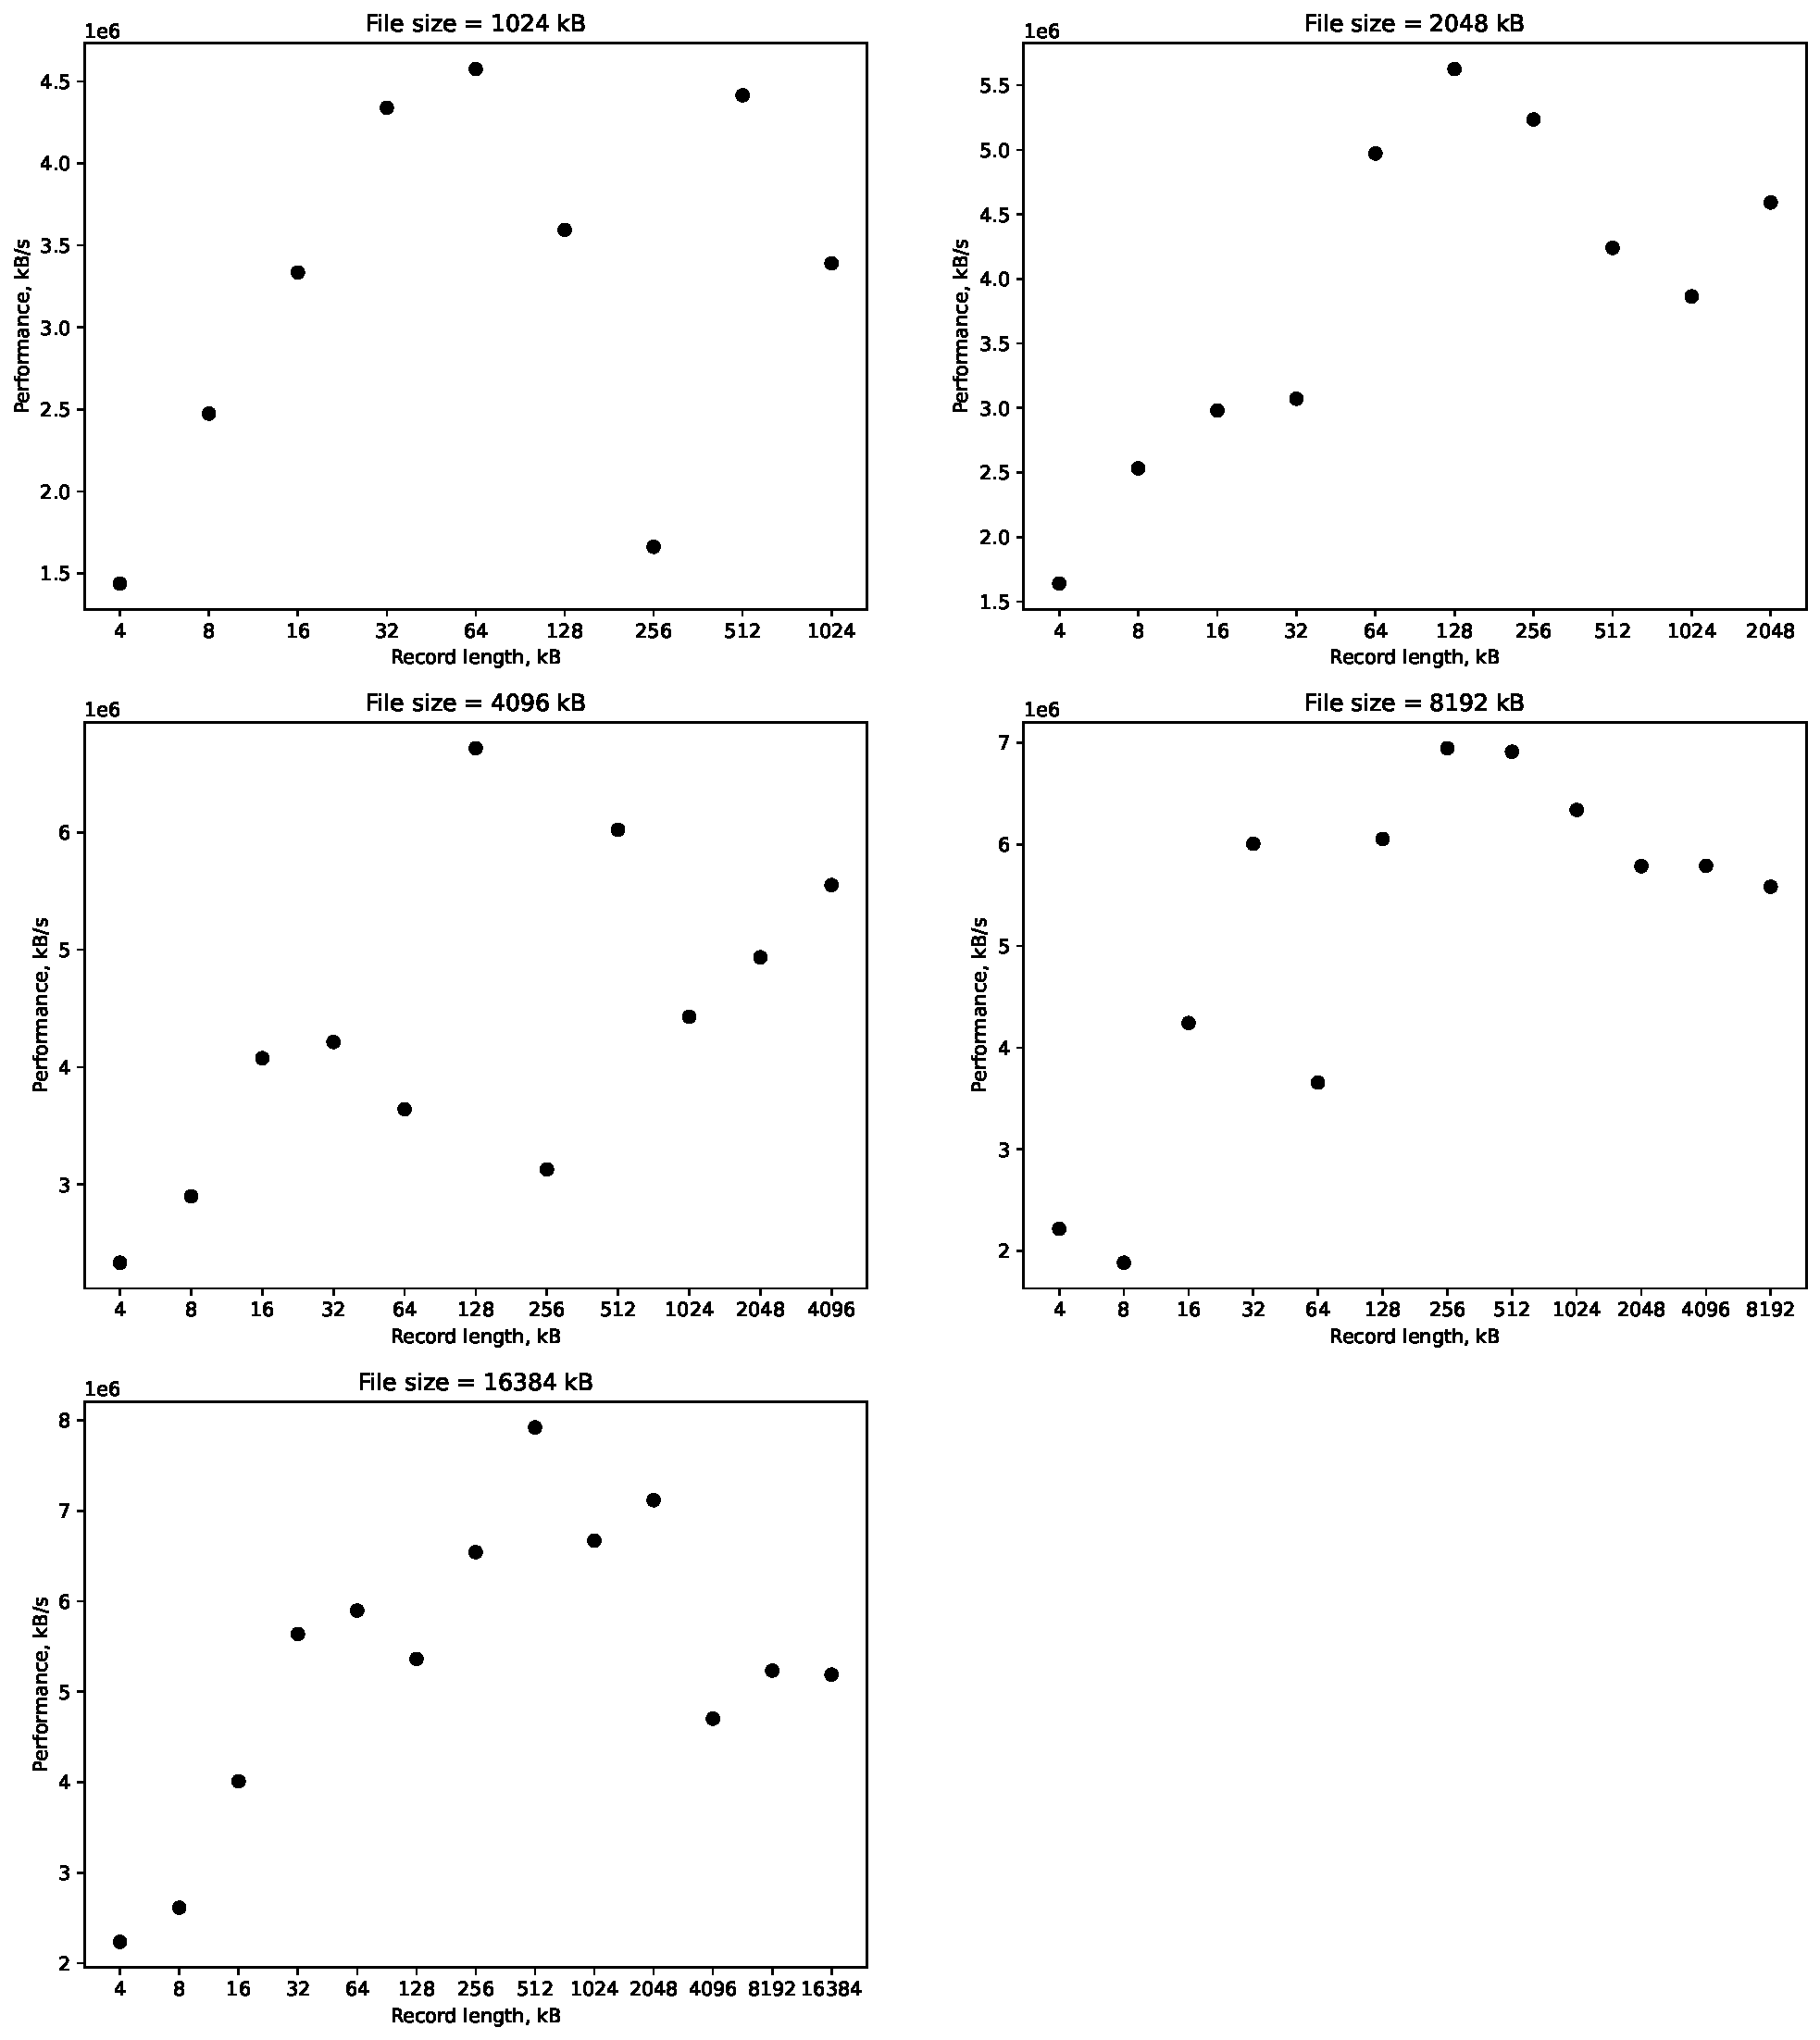
\includegraphics[width=1.0\textwidth]{figures/benchmarking/fejk-ffs/Random read.pdf}
	\end{center}
	\caption{IOZone output for Fejk FFS Random read}
\end{figure}

\begin{figure}[!htb]
	\label{fig:bench_fffs_rnd_write}
	\begin{center}
		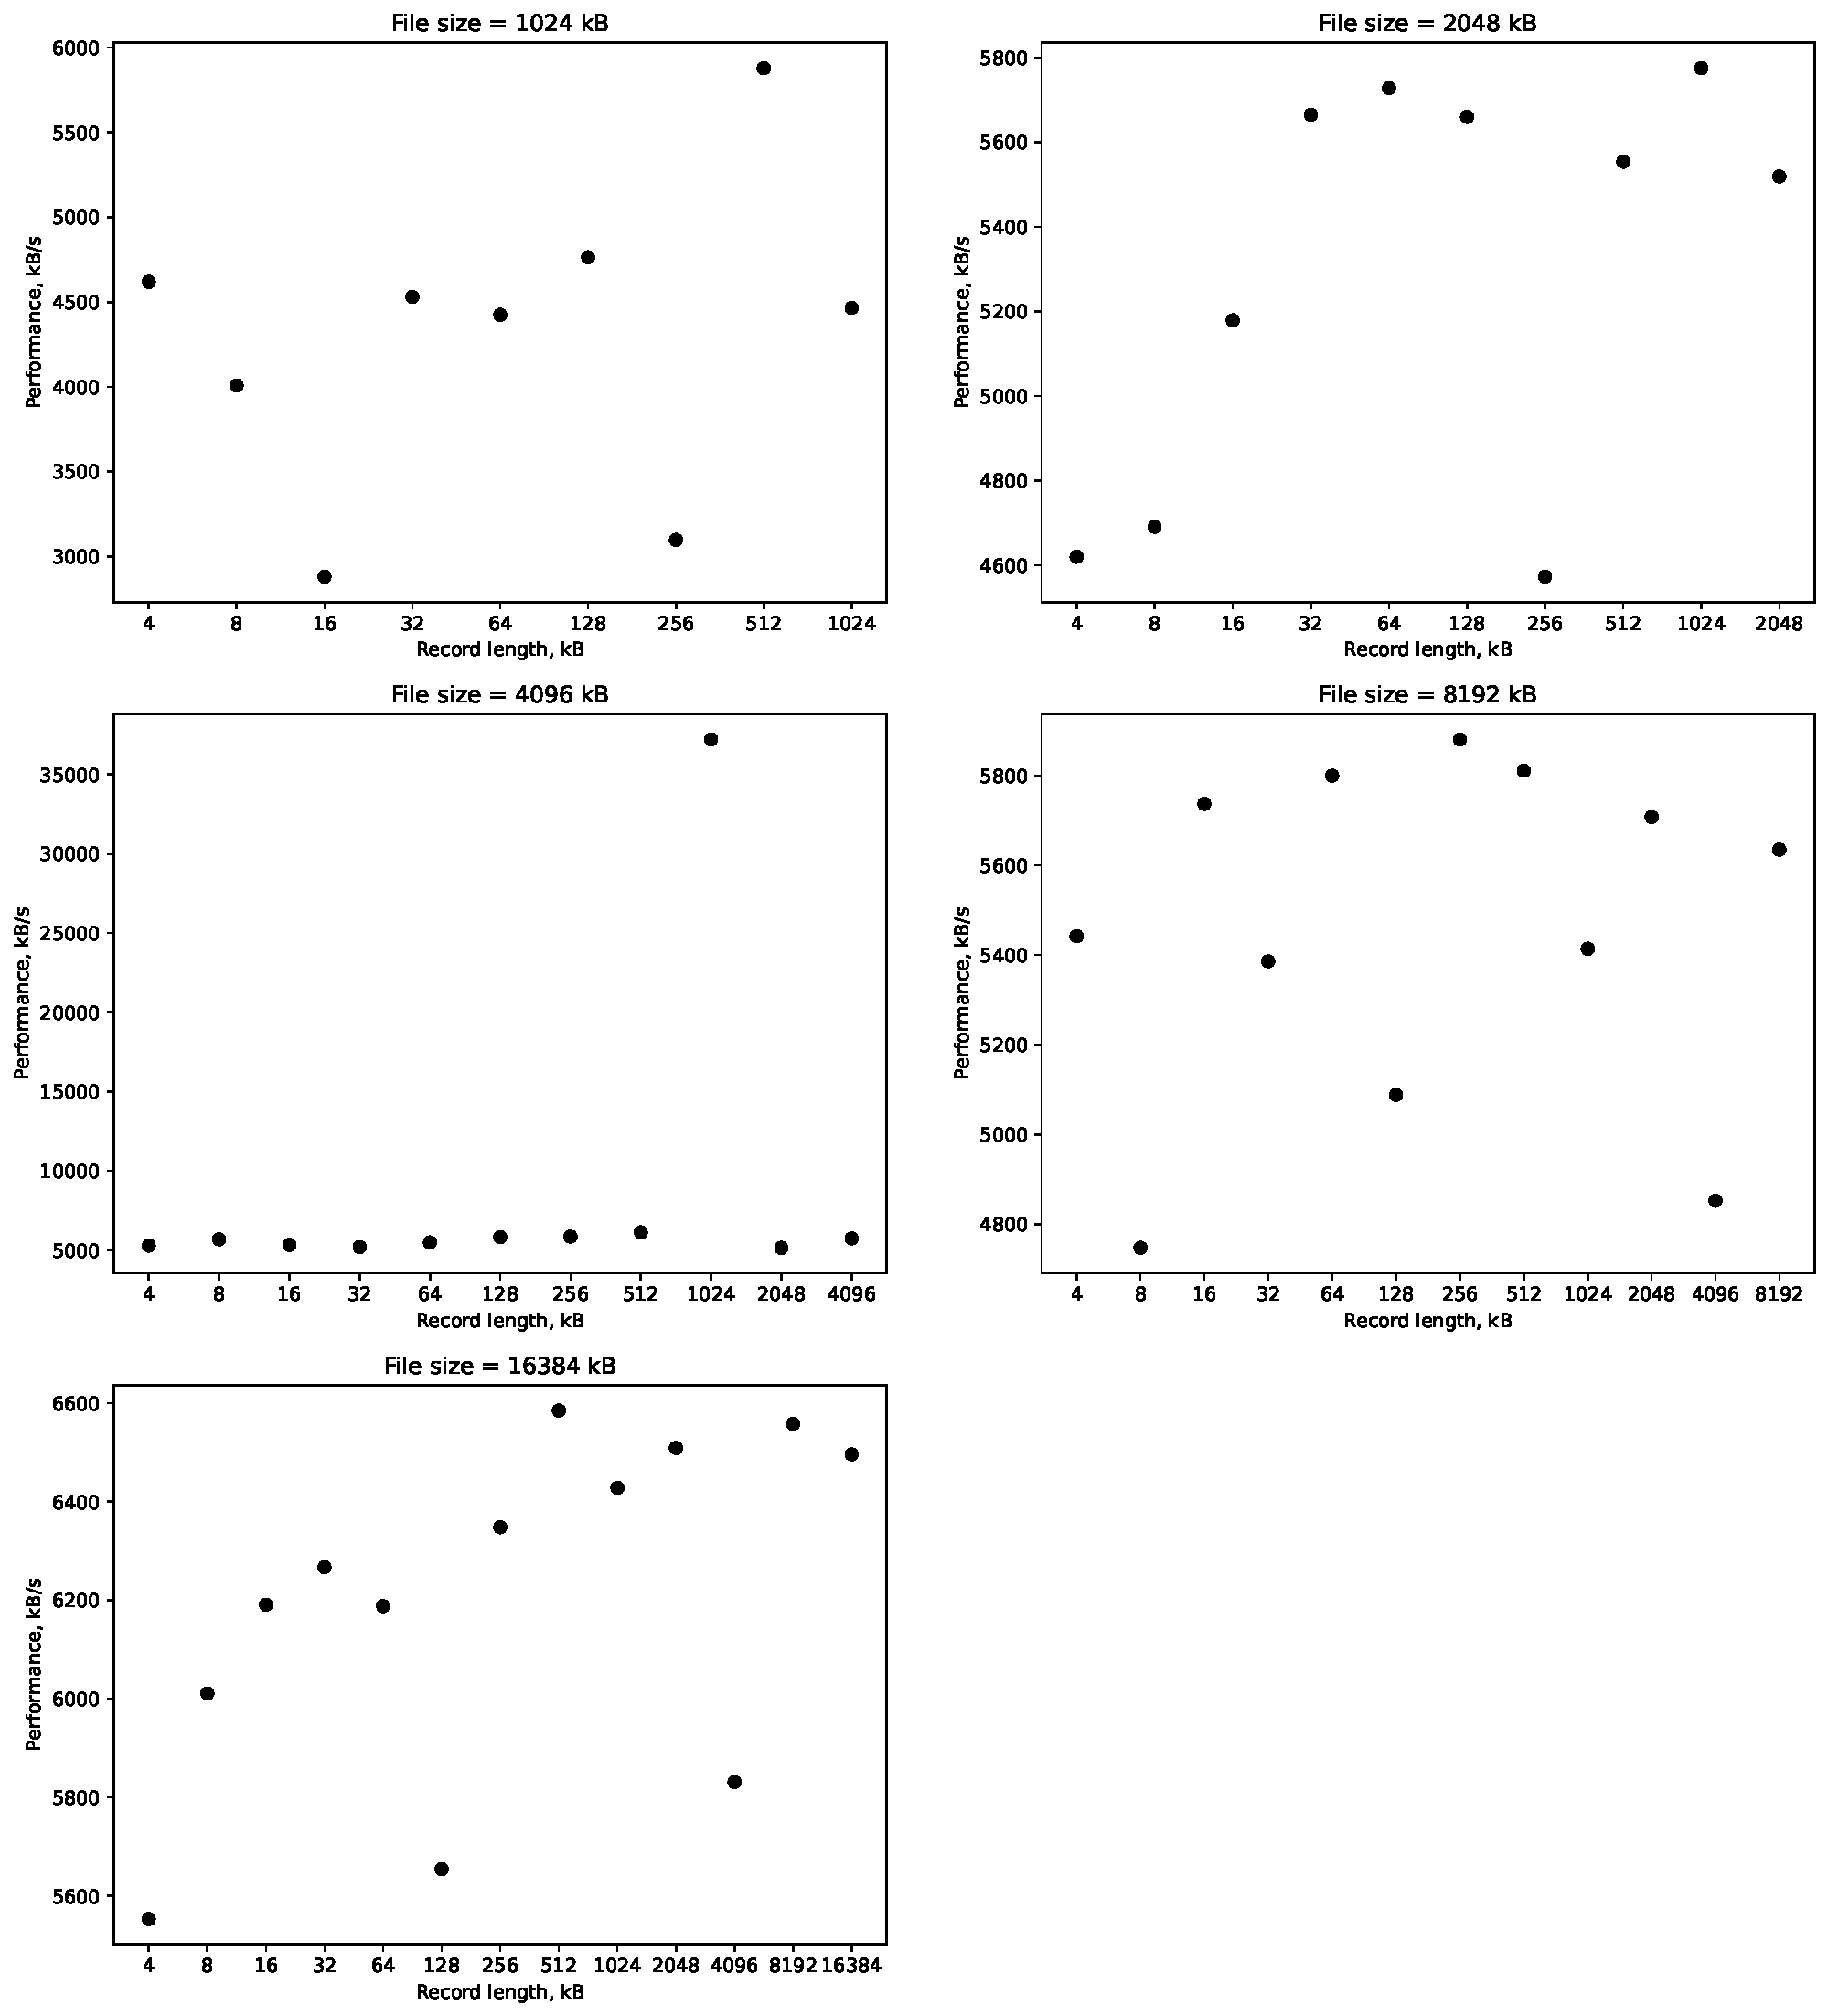
\includegraphics[width=1.0\textwidth]{figures/benchmarking/fejk-ffs/Random write.pdf}
	\end{center}
	\caption{IOZone output for Fejk FFS Random write}
\end{figure}

\FloatBarrier

Figure~\ref{fig:bench_gcsf_read}, Figure~\ref{fig:bench_gcsf_write}, Figure~\ref{fig:bench_gcsf_re_read}, Figure~\ref{fig:bench_gcsf_re_write}, Figure~\ref{fig:bench_gcsf_rnd_read}, and Figure~\ref{fig:bench_gcsf_rnd_write} presents the performances of the Read, Write, \mbox{Re-Read}, \mbox{Re-Write}, Random Read, and Random Write tests for \gls{GCSF}.

\begin{figure}[!htb]
	\label{fig:bench_gcsf_read}
	\begin{center}
		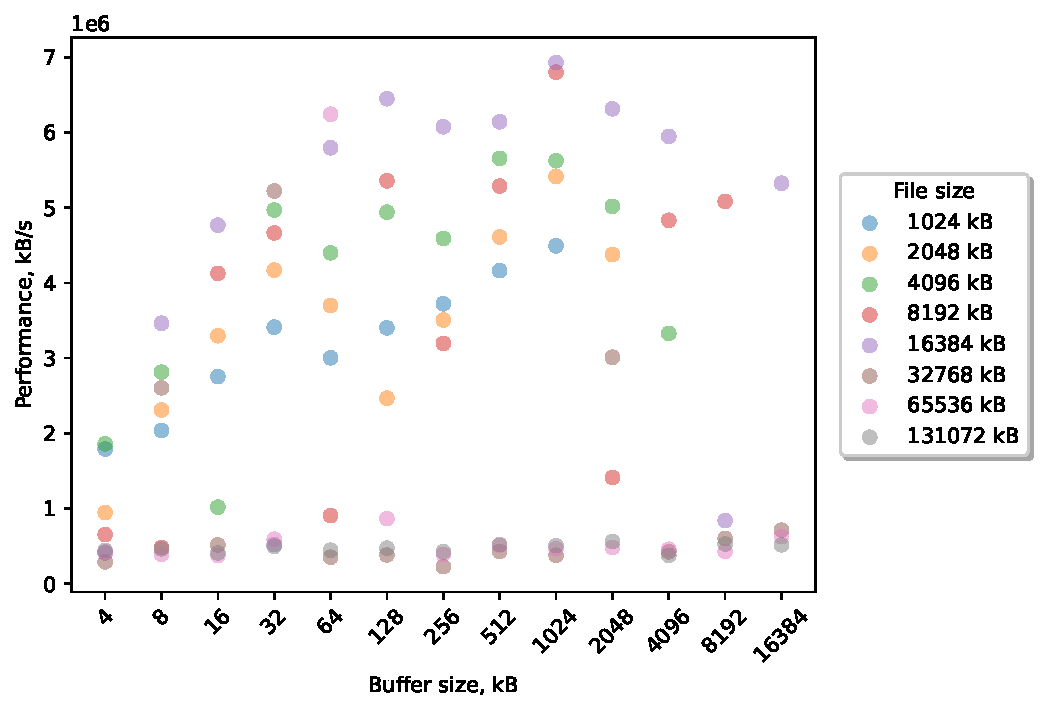
\includegraphics[width=1.0\textwidth]{figures/benchmarking/gcsf/Read.pdf}
	\end{center}
	\caption{IOZone output for GCSF Read}
\end{figure}

\begin{figure}[!htb]
	\label{fig:bench_gcsf_write}
	\begin{center}
		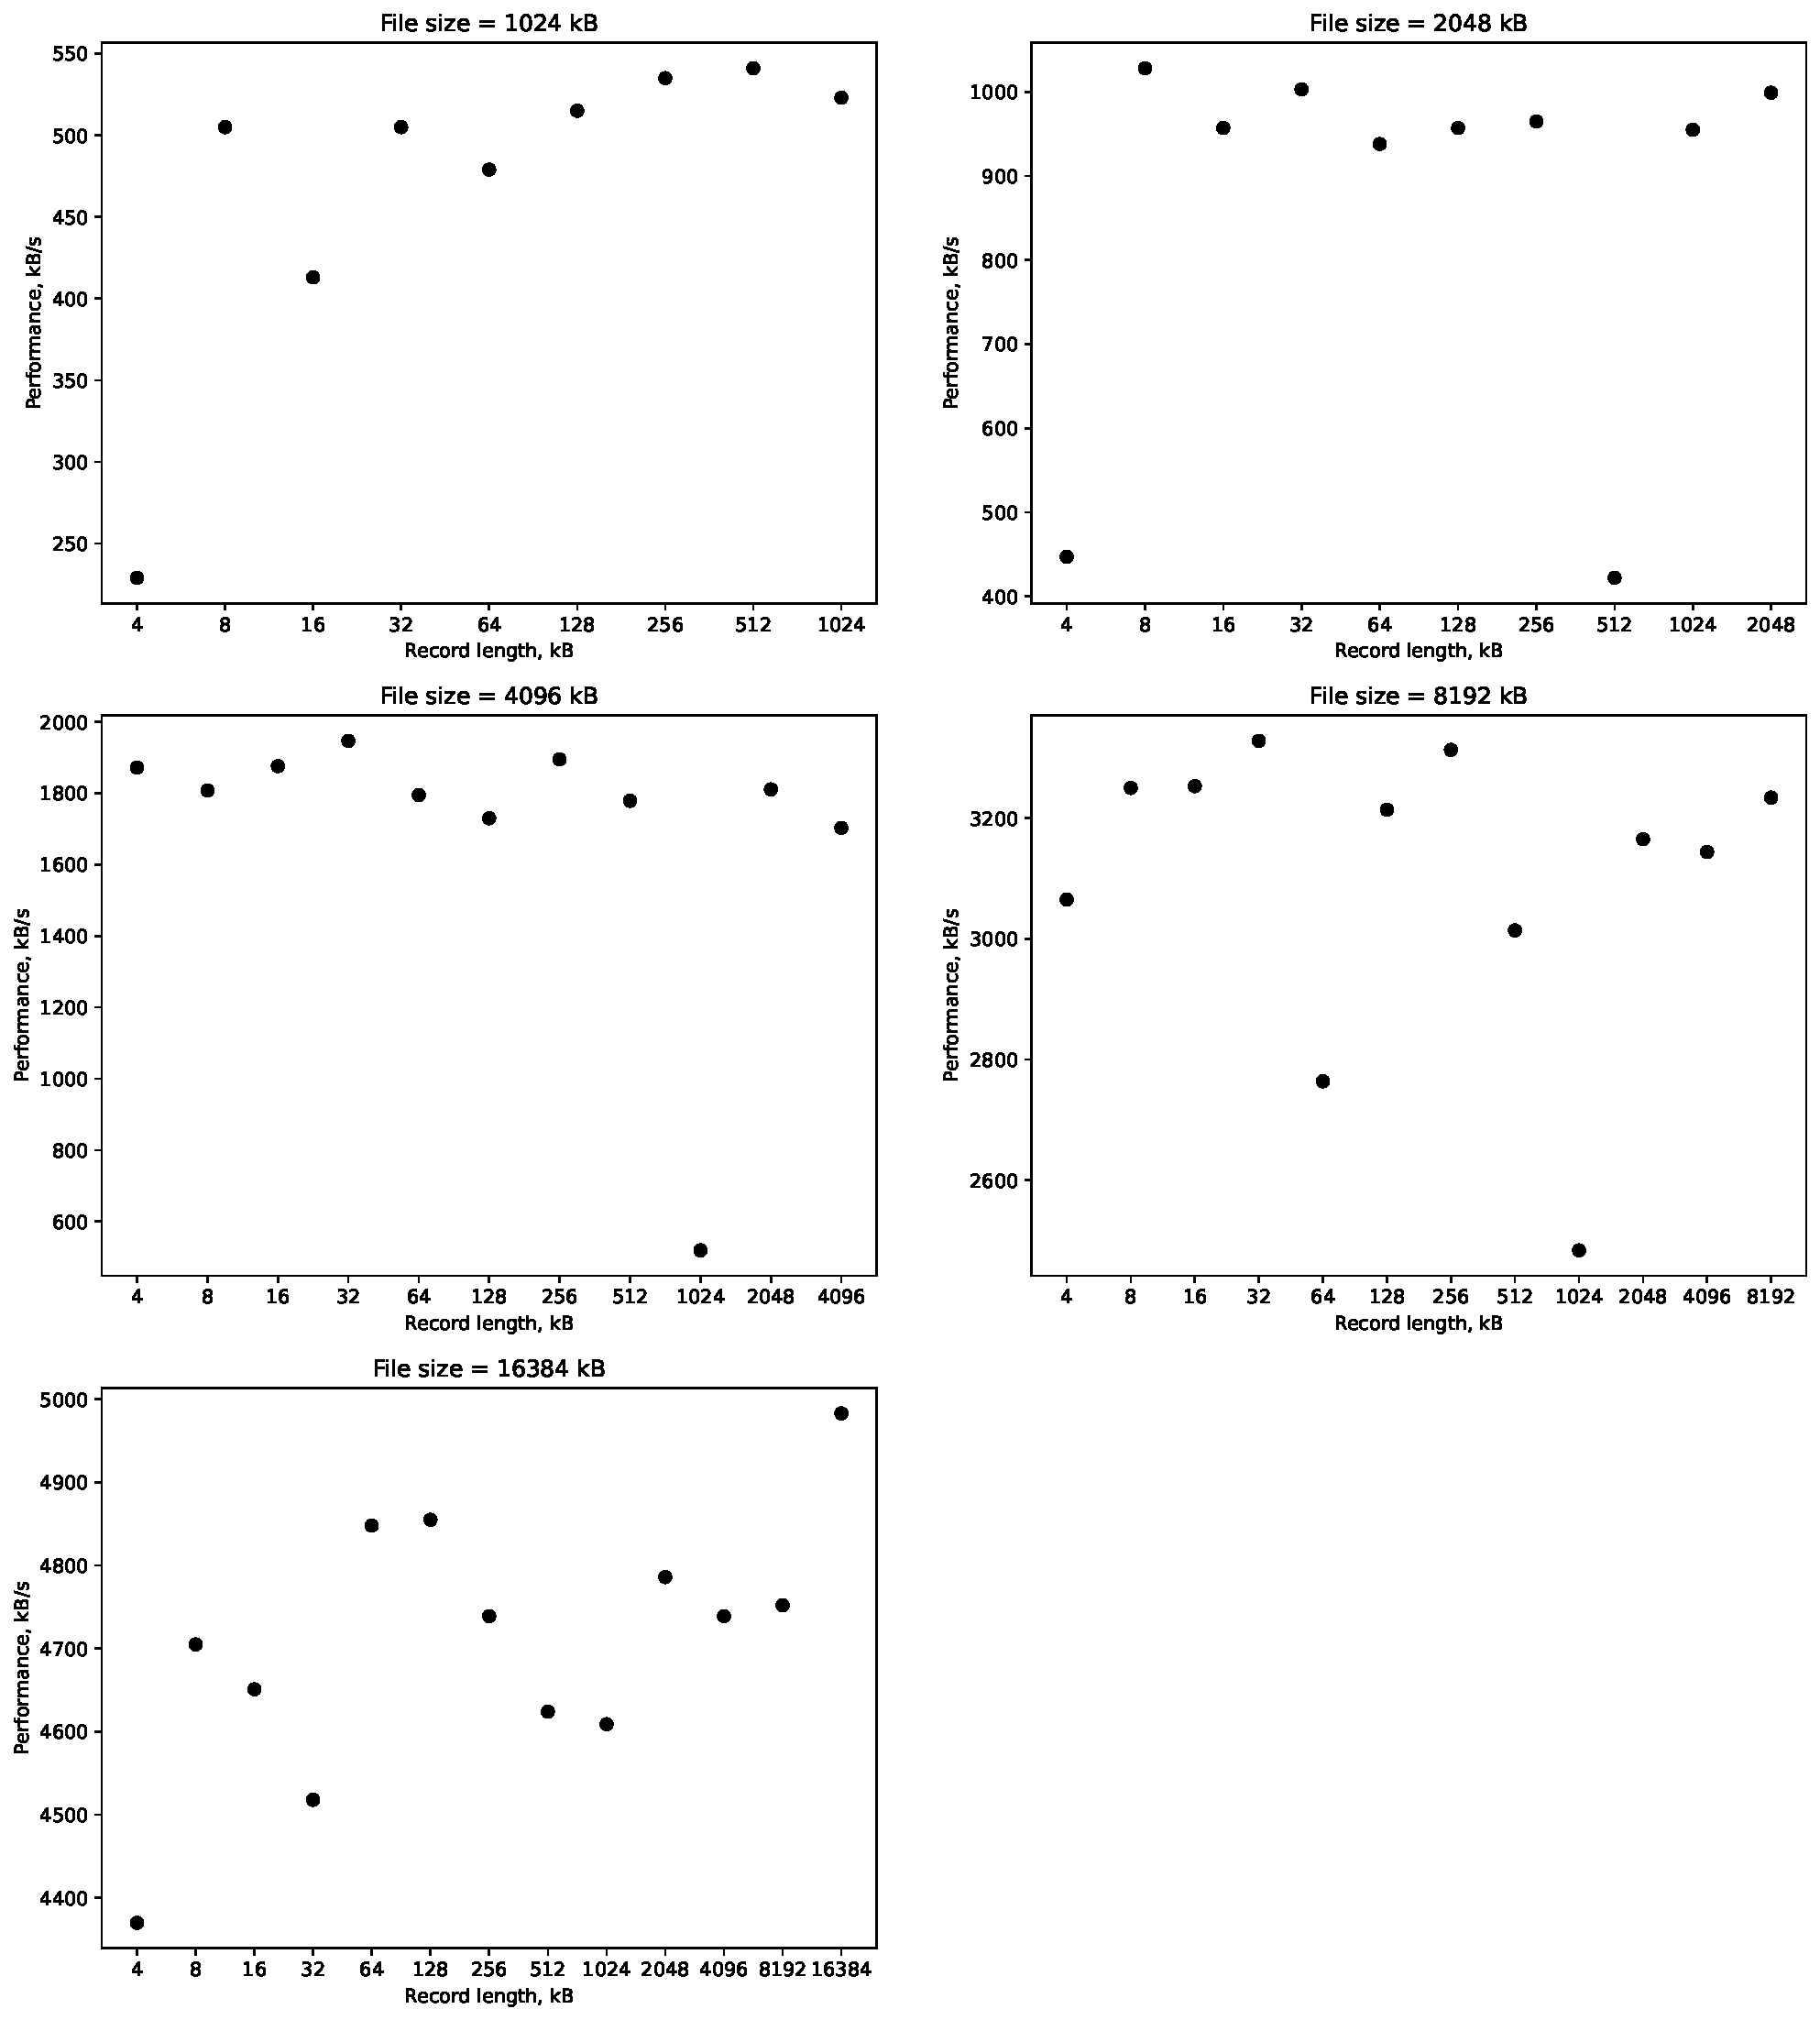
\includegraphics[width=1.0\textwidth]{figures/benchmarking/gcsf/Write.pdf}
	\end{center}
	\caption{IOZone output for GCSF Write}
\end{figure}

\begin{figure}[!htb]
	\label{fig:bench_gcsf_re_read}
	\begin{center}
		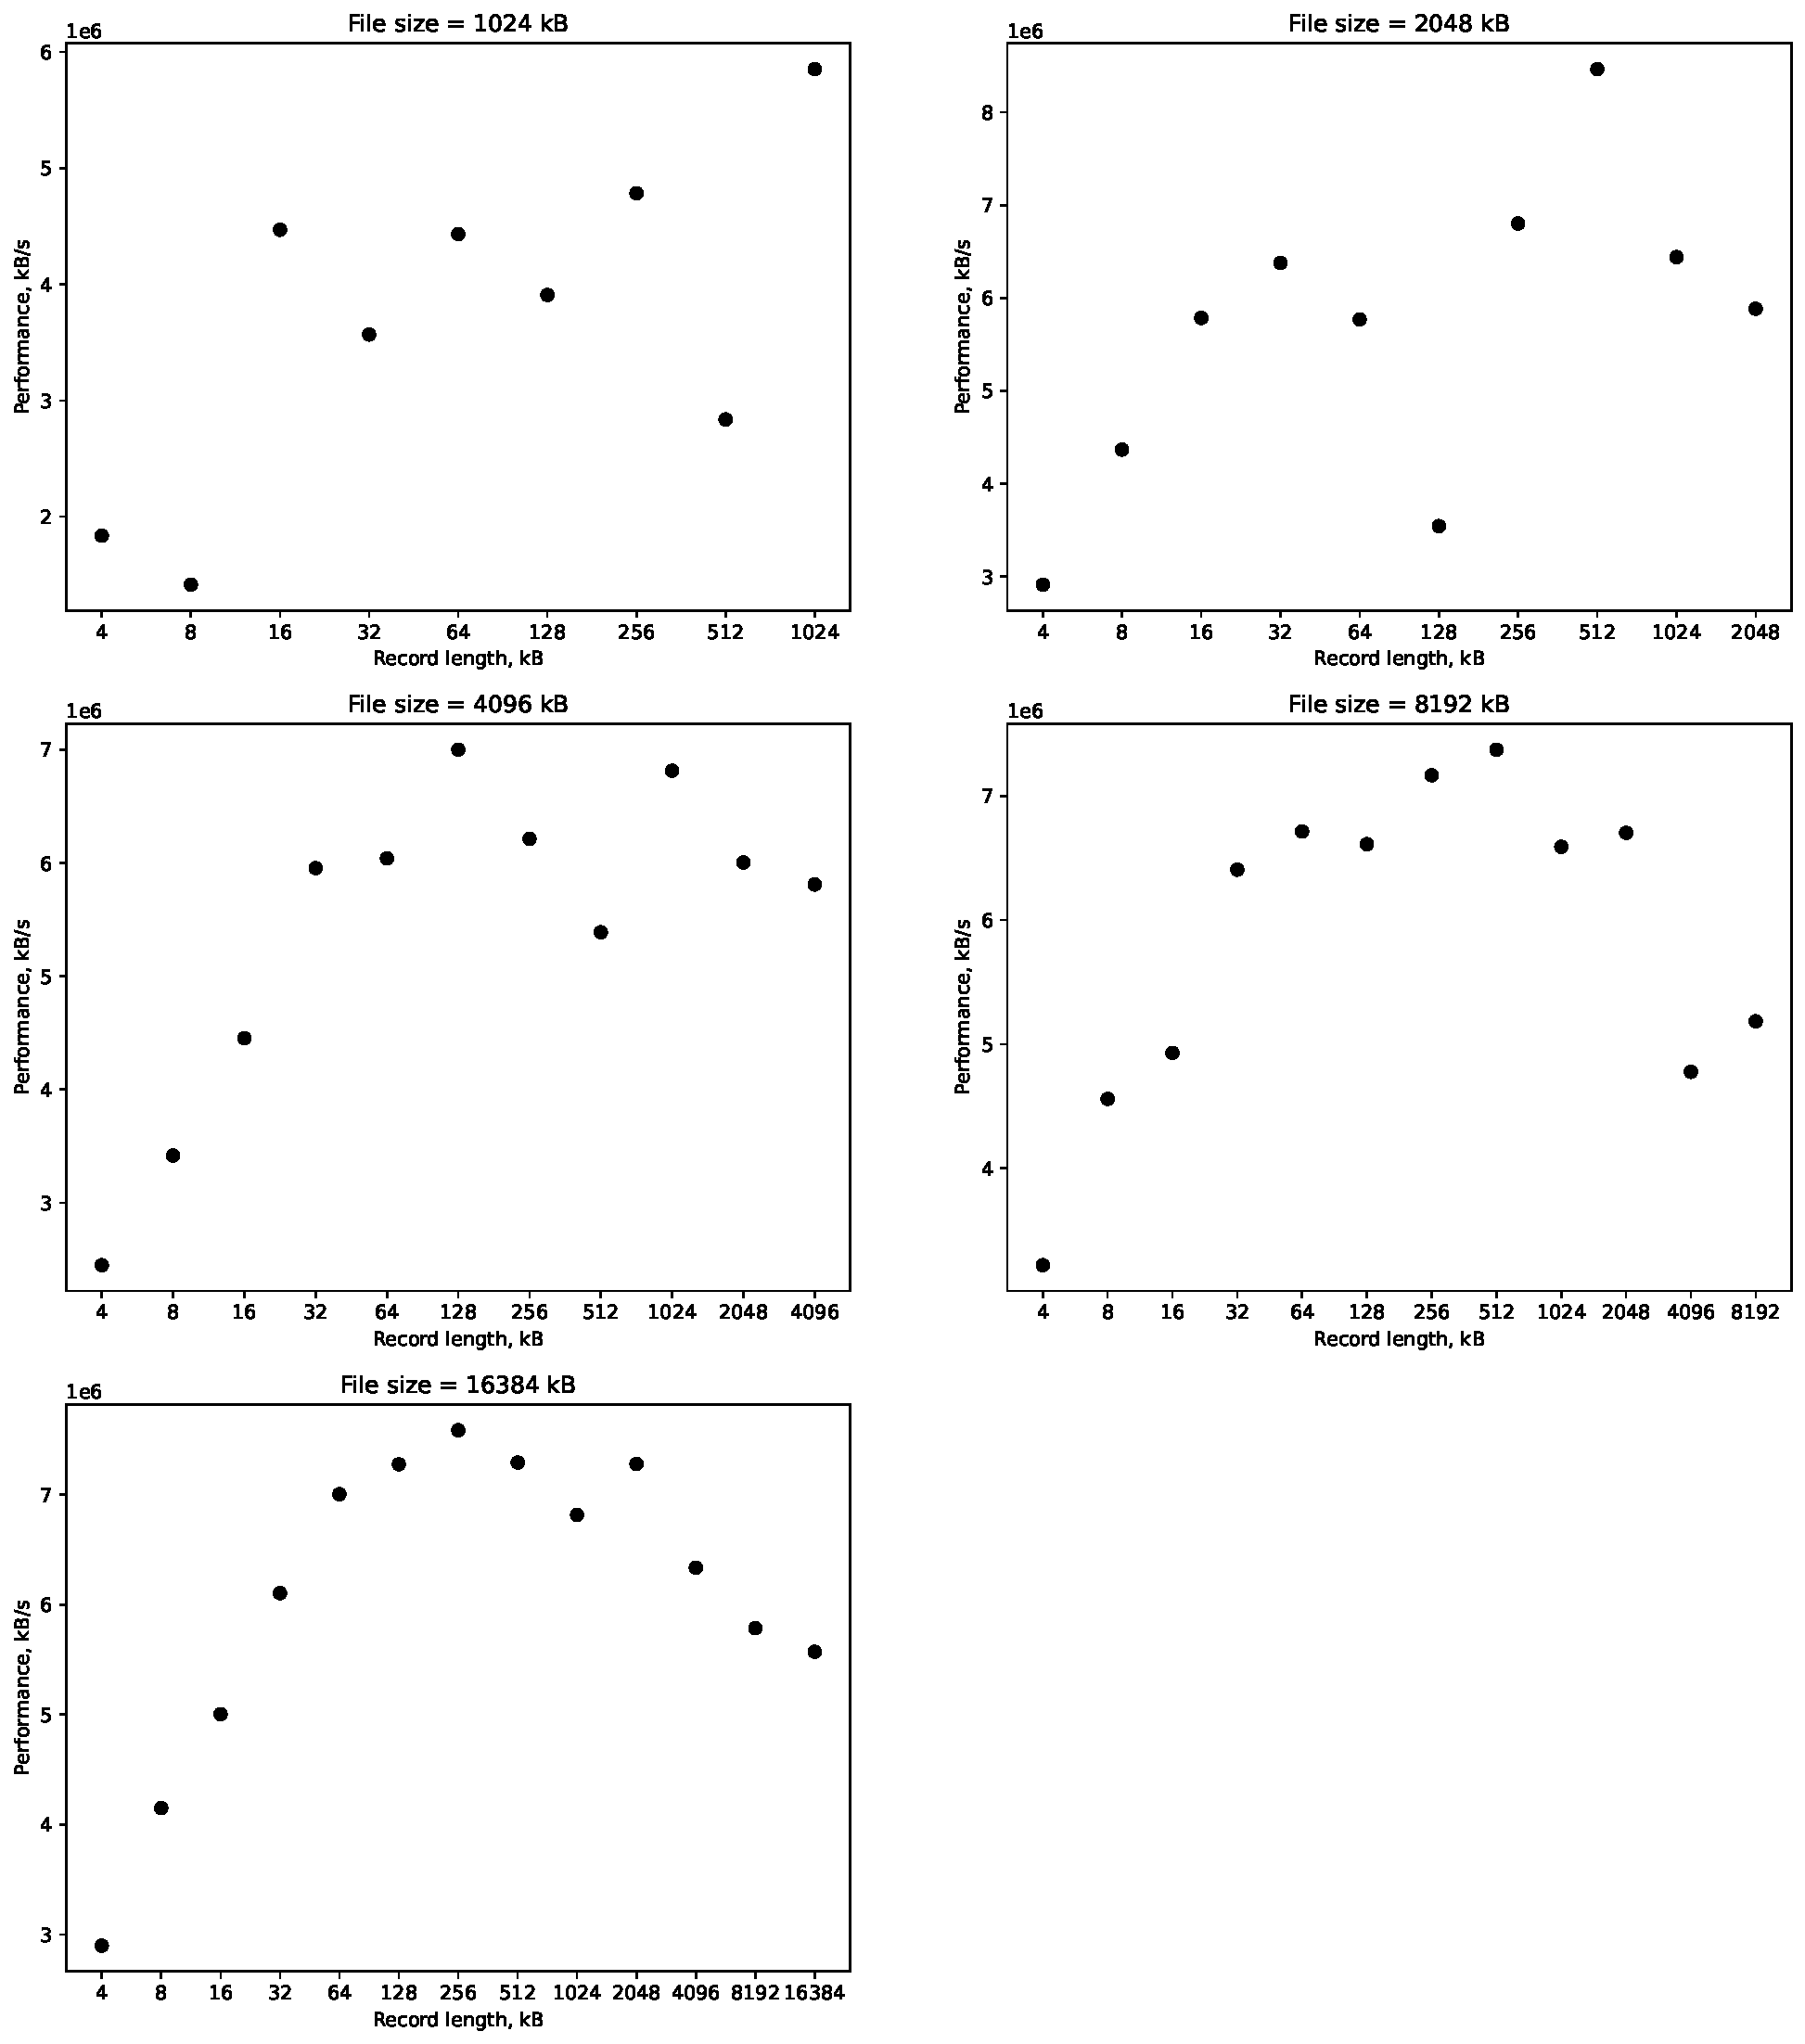
\includegraphics[width=1.0\textwidth]{figures/benchmarking/gcsf/Re-Read.pdf}
	\end{center}
	\caption{IOZone output for GCSF \mbox{Re-Read}}
\end{figure}

\begin{figure}[!htb]
	\label{fig:bench_gcsf_re_write}
	\begin{center}
		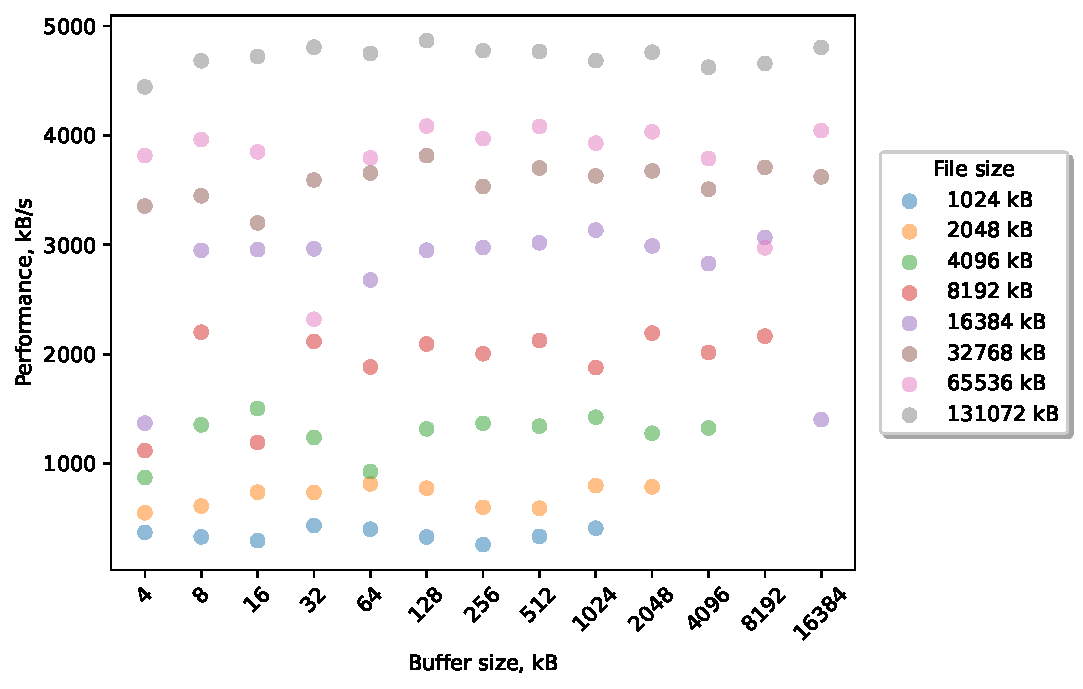
\includegraphics[width=1.0\textwidth]{figures/benchmarking/gcsf/Re-Write.pdf}
	\end{center}
	\caption{IOZone output for GCSF \mbox{Re-Write}}
\end{figure}

\begin{figure}[!htb]
	\label{fig:bench_gcsf_rnd_read}
	\begin{center}
		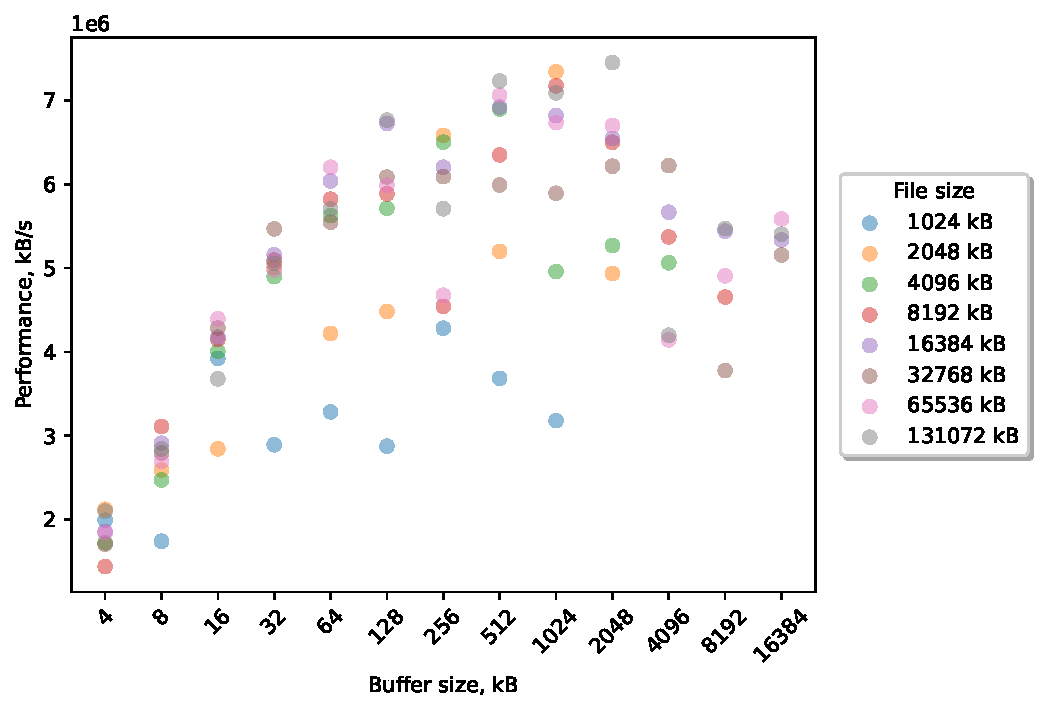
\includegraphics[width=1.0\textwidth]{figures/benchmarking/gcsf/Random read.pdf}
	\end{center}
	\caption{IOZone output for GCSF Random read}
\end{figure}

\begin{figure}[!htb]
	\label{fig:bench_gcsf_rnd_write}
	\begin{center}
		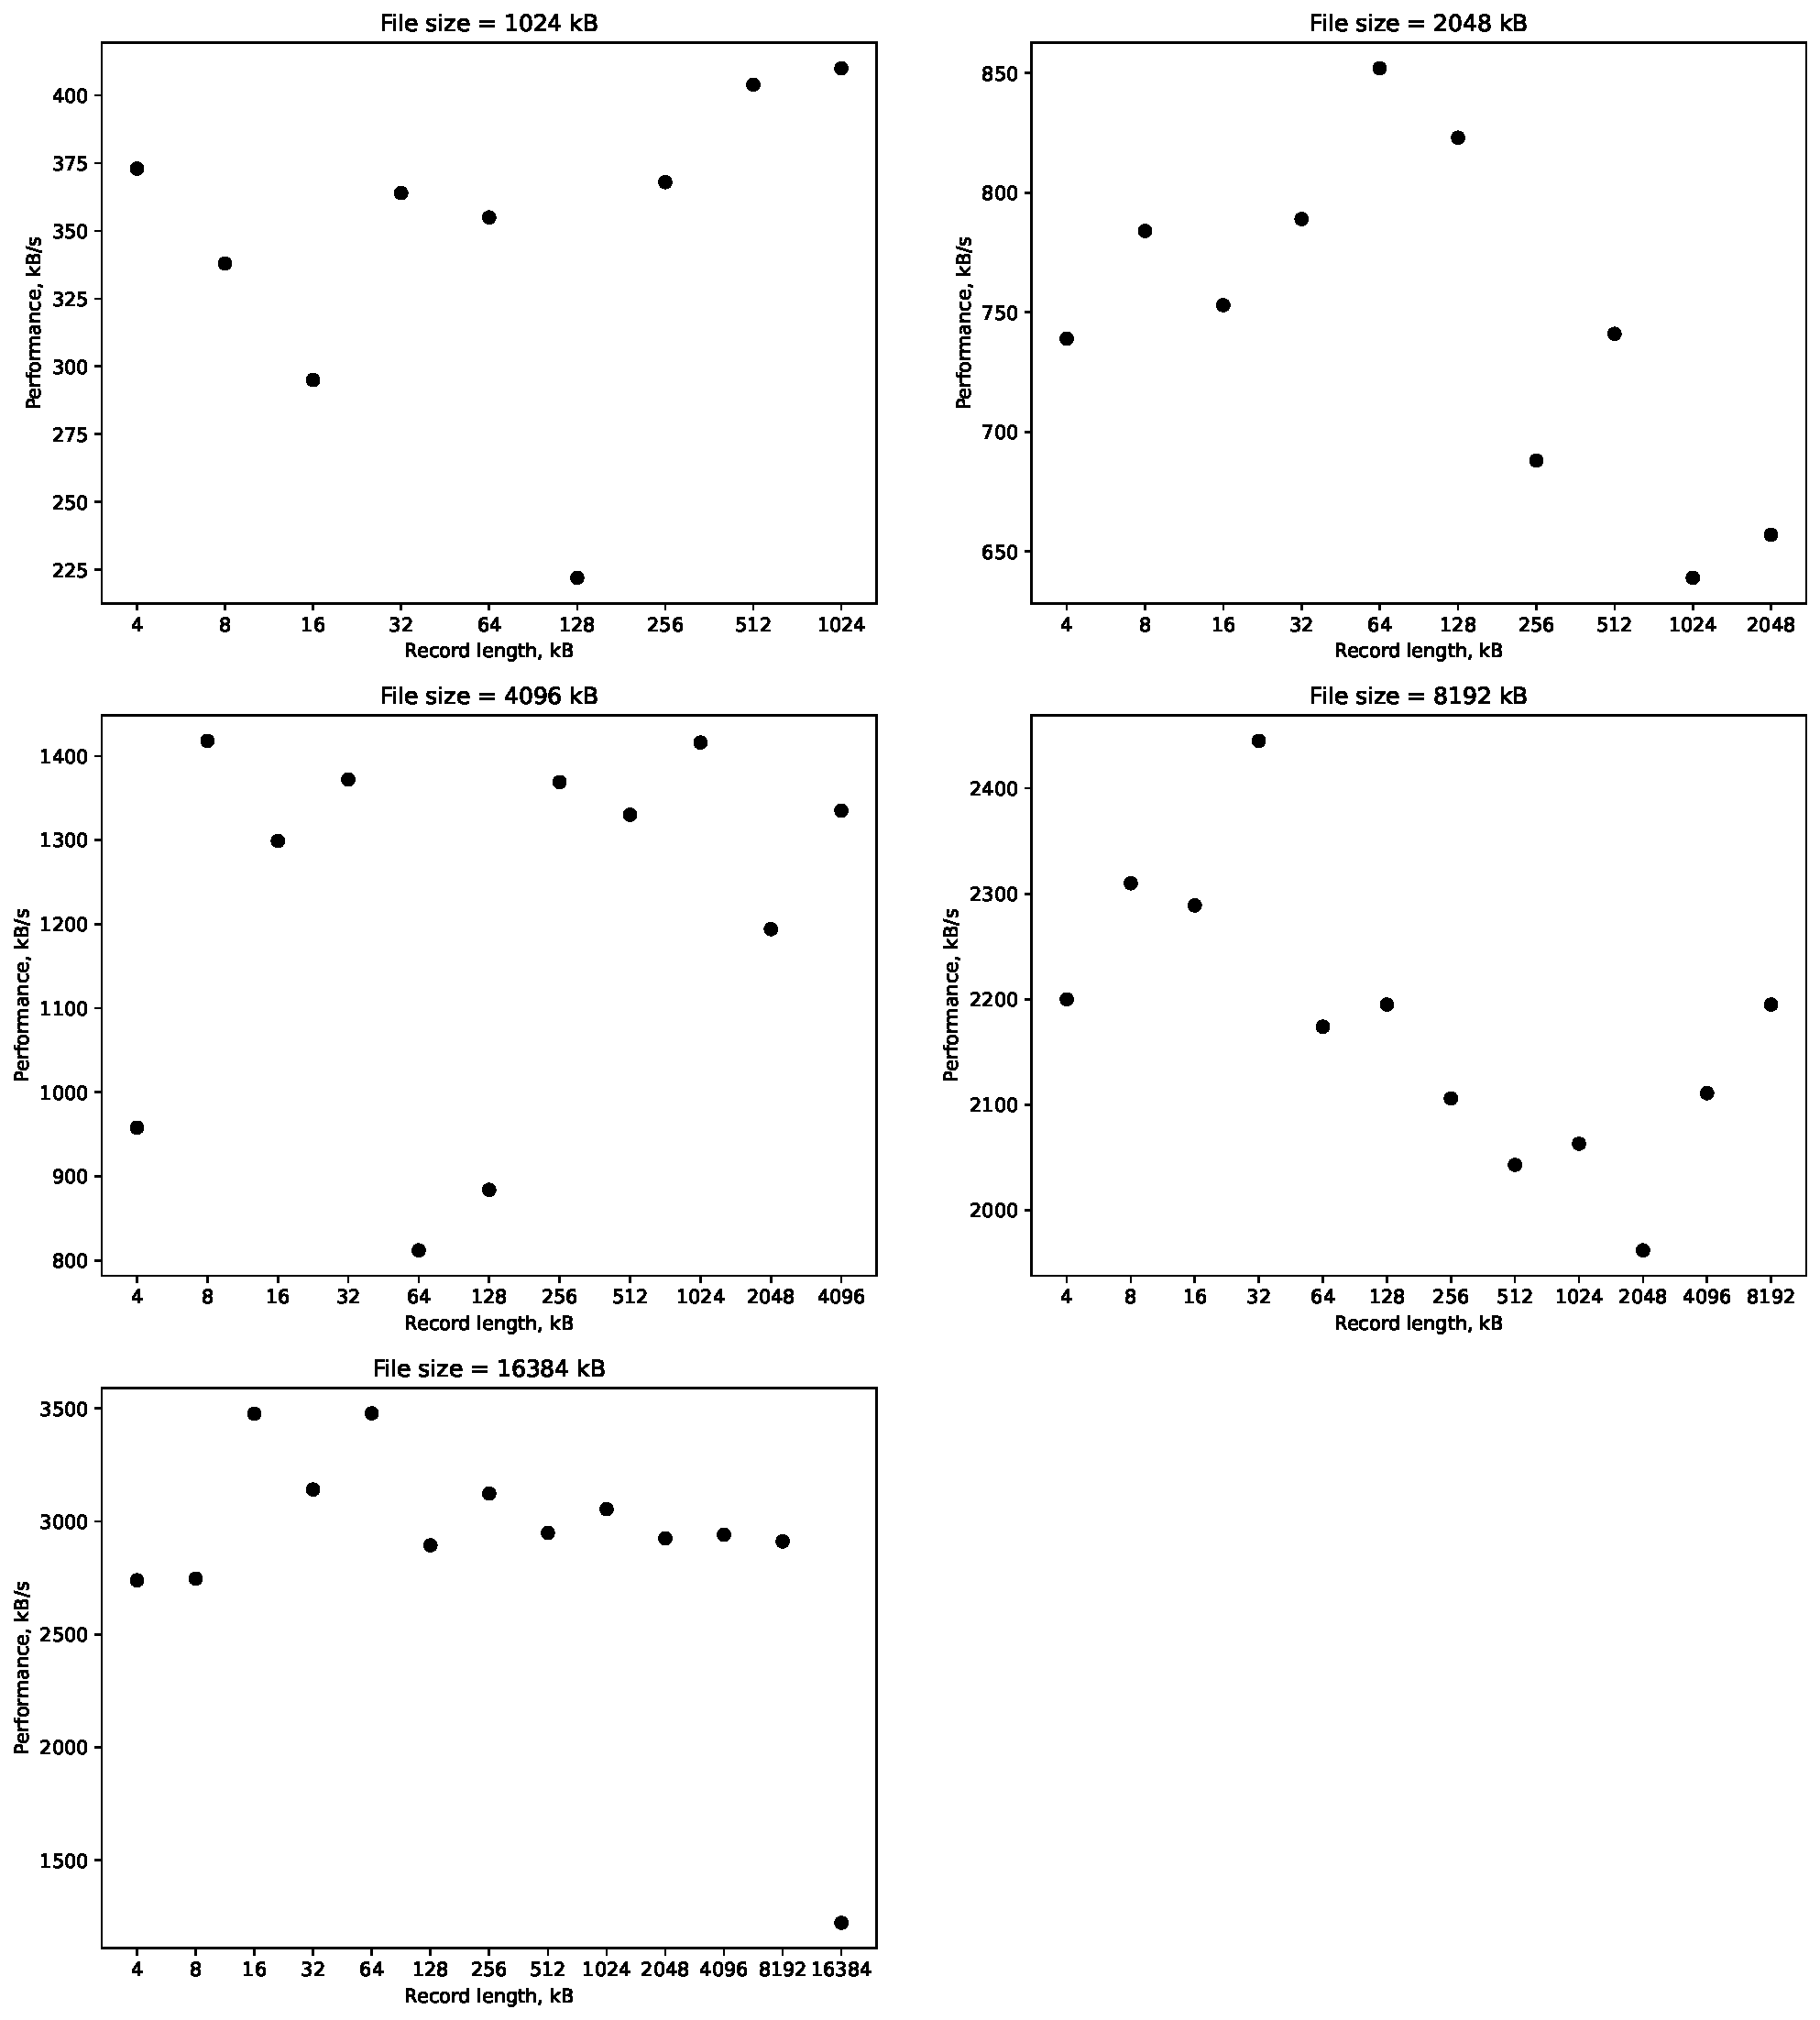
\includegraphics[width=1.0\textwidth]{figures/benchmarking/gcsf/Random write.pdf}
	\end{center}
	\caption{IOZone output for GCSF Random write}
\end{figure}

\FloatBarrier

Figure~\ref{fig:bench_apfs_read}, Figure~\ref{fig:bench_apfs_write}, Figure~\ref{fig:bench_apfs_re_read}, Figure~\ref{fig:bench_apfs_re_write}, Figure~\ref{fig:bench_apfs_rnd_read}, and Figure~\ref{fig:bench_apfs_rnd_write} presents the performances of the Read, Write, \mbox{Re-Read}, \mbox{Re-Write}, Random Read, and Random Write tests for \gls{APFS}.

\begin{figure}[!htb]
	\label{fig:bench_apfs_read}
	\begin{center}
		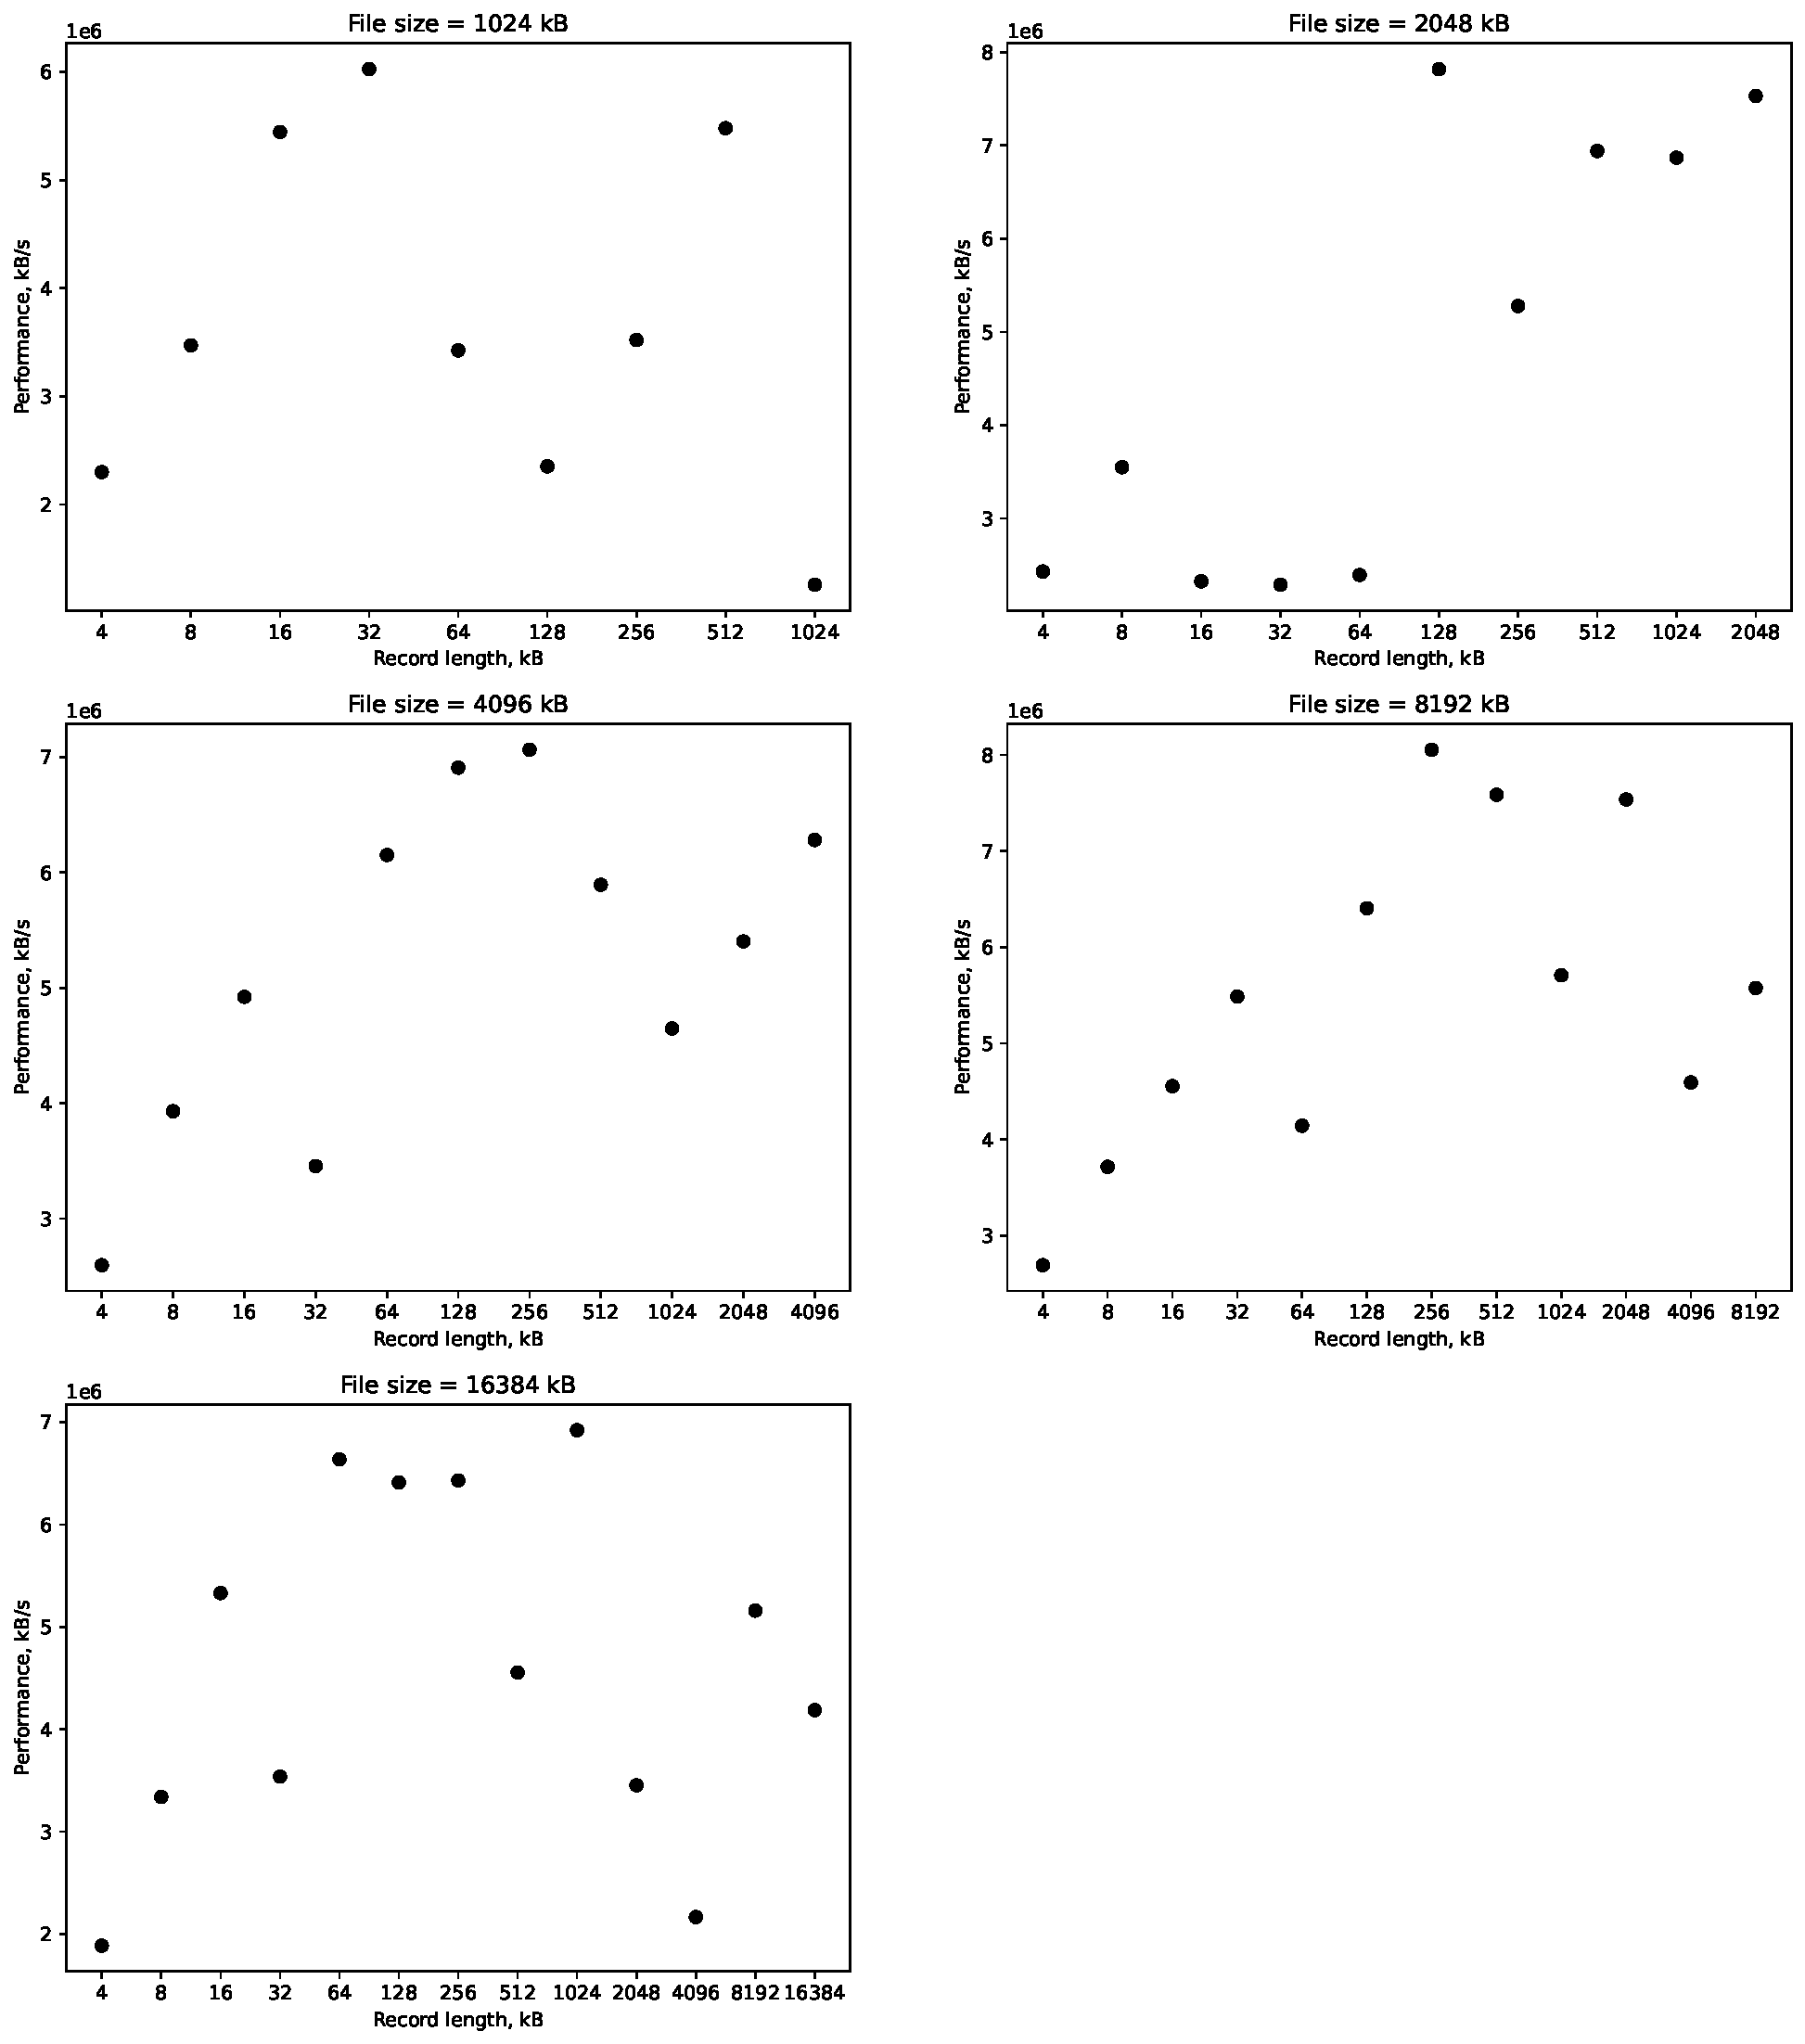
\includegraphics[width=1.0\textwidth]{figures/benchmarking/local/Read.pdf}
	\end{center}
	\caption{IOZone output for \gls{APFS} Read}
\end{figure}

\begin{figure}[!htb]
	\label{fig:bench_apfs_write}
	\begin{center}
		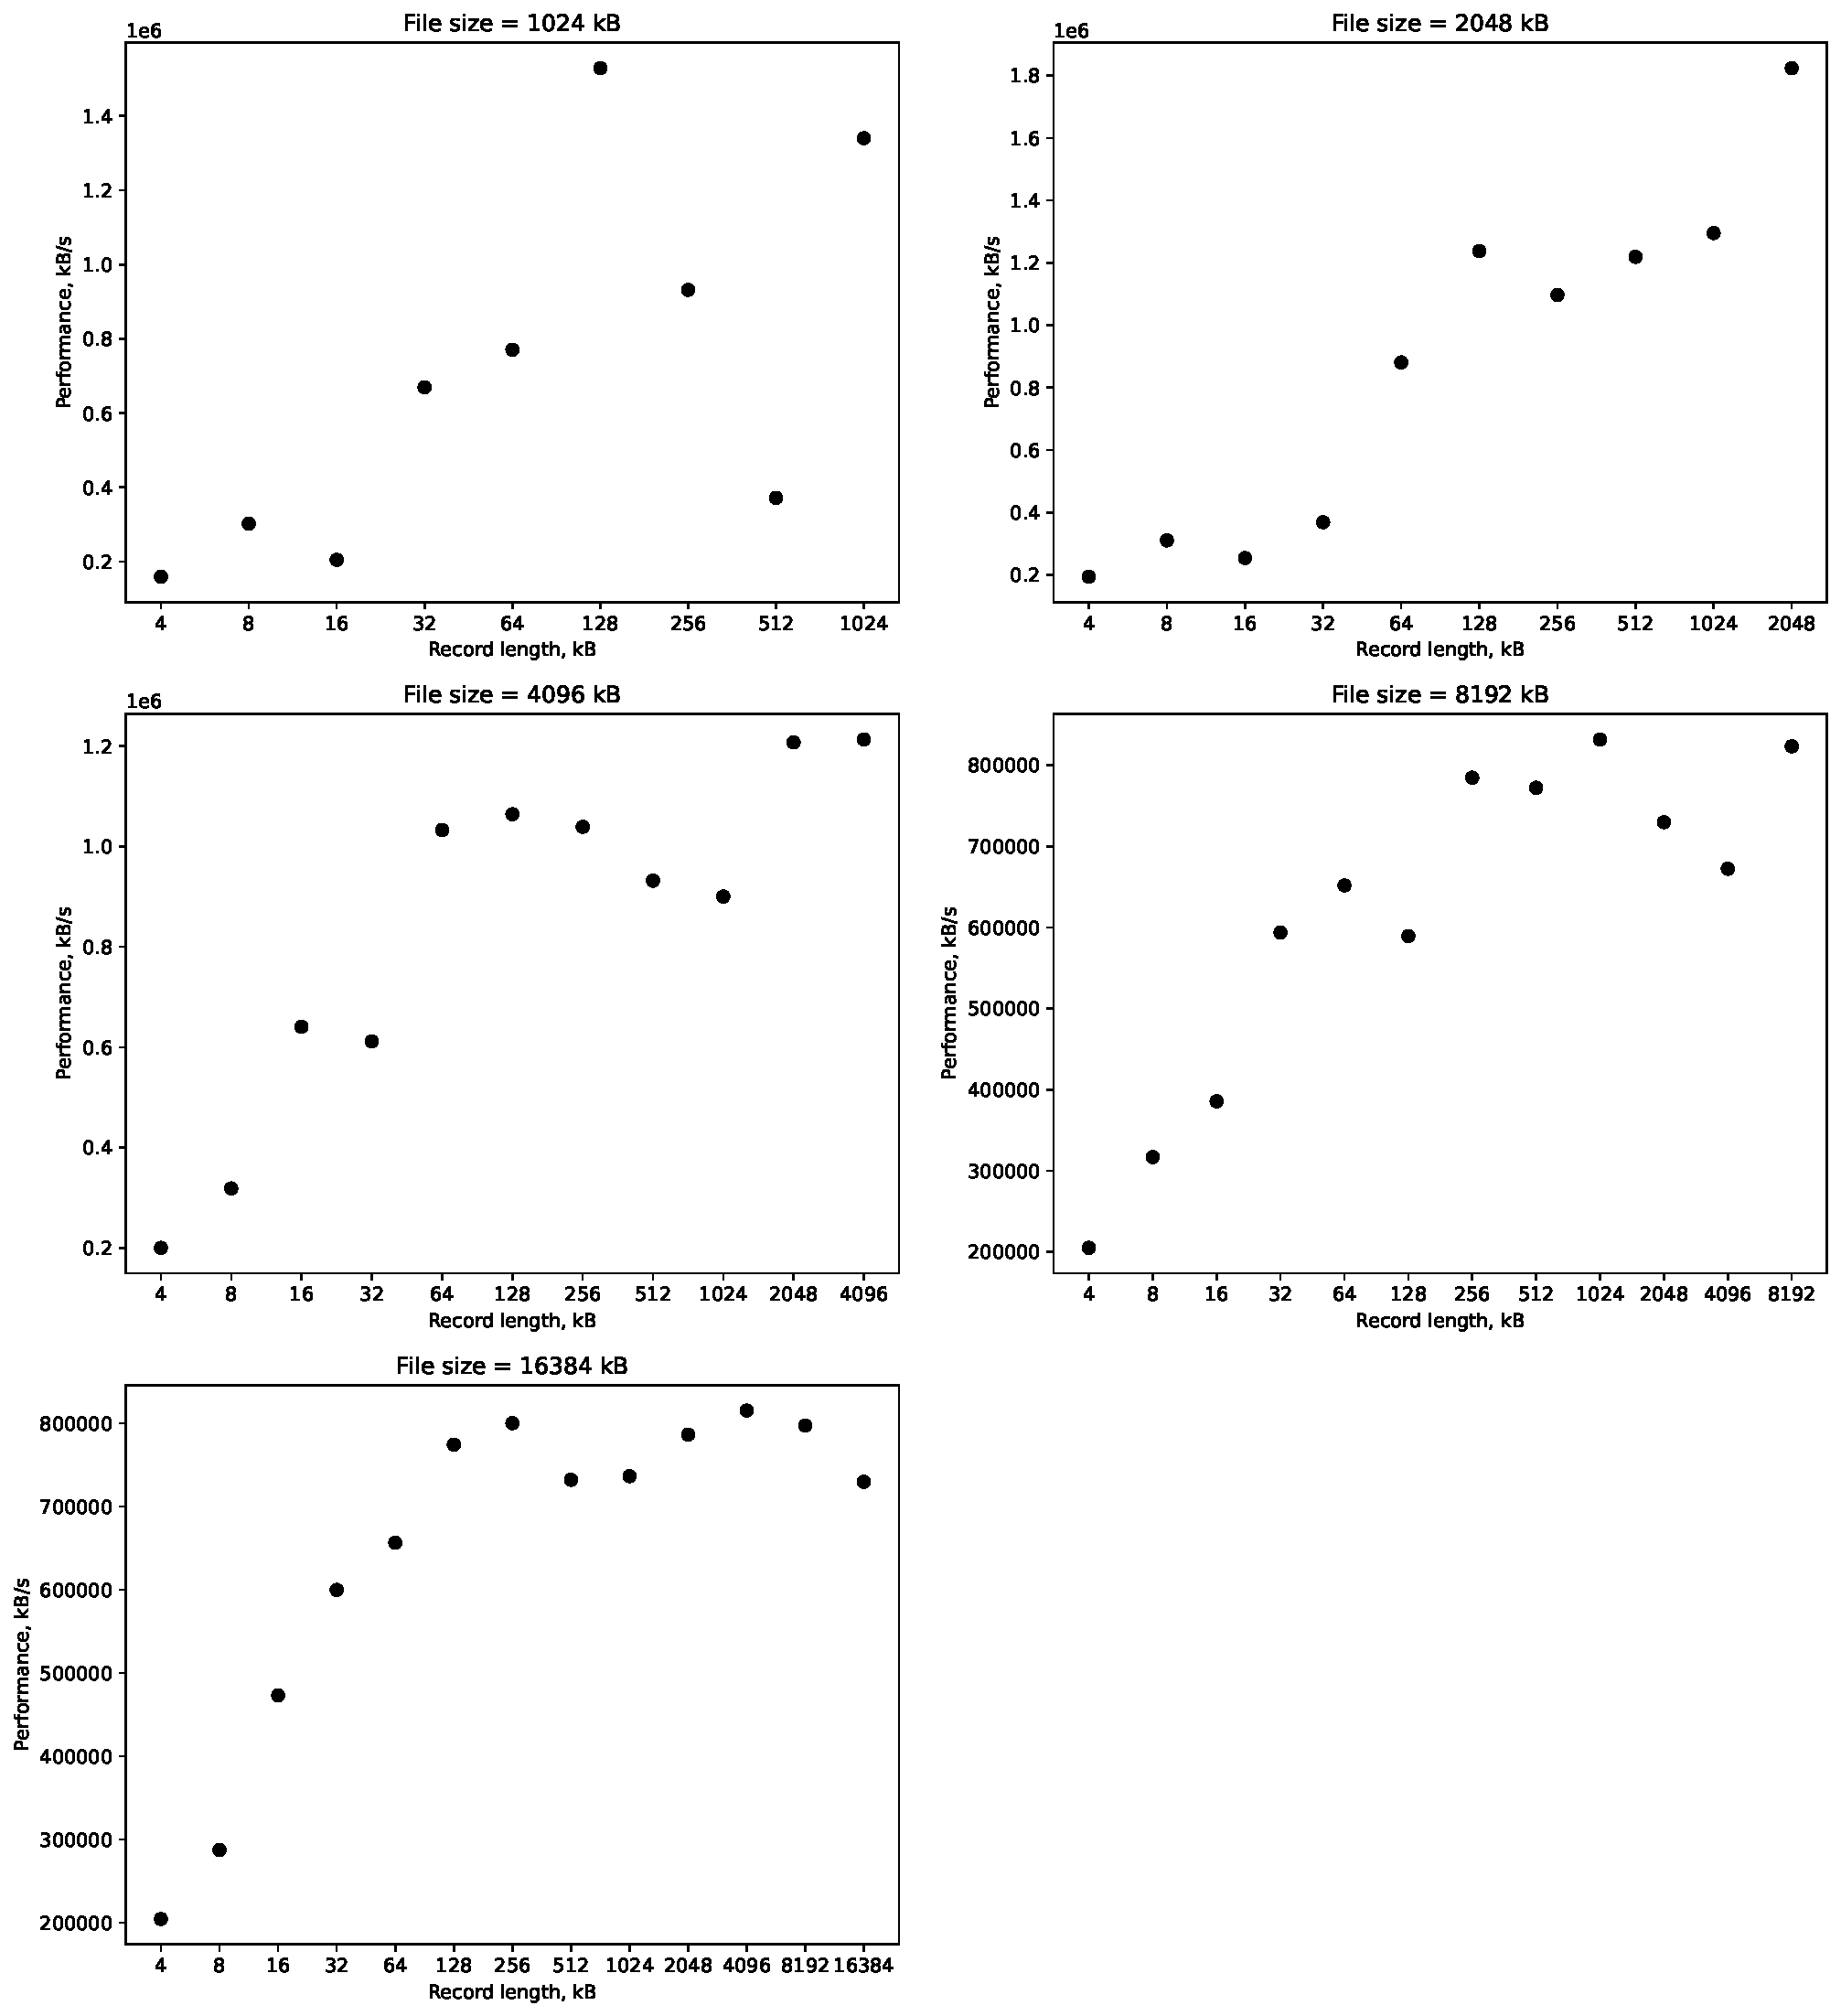
\includegraphics[width=1.0\textwidth]{figures/benchmarking/local/Write.pdf}
	\end{center}
	\caption{IOZone output for \gls{APFS} Write}
\end{figure}

\begin{figure}[!htb]
	\label{fig:bench_apfs_re_read}
	\begin{center}
		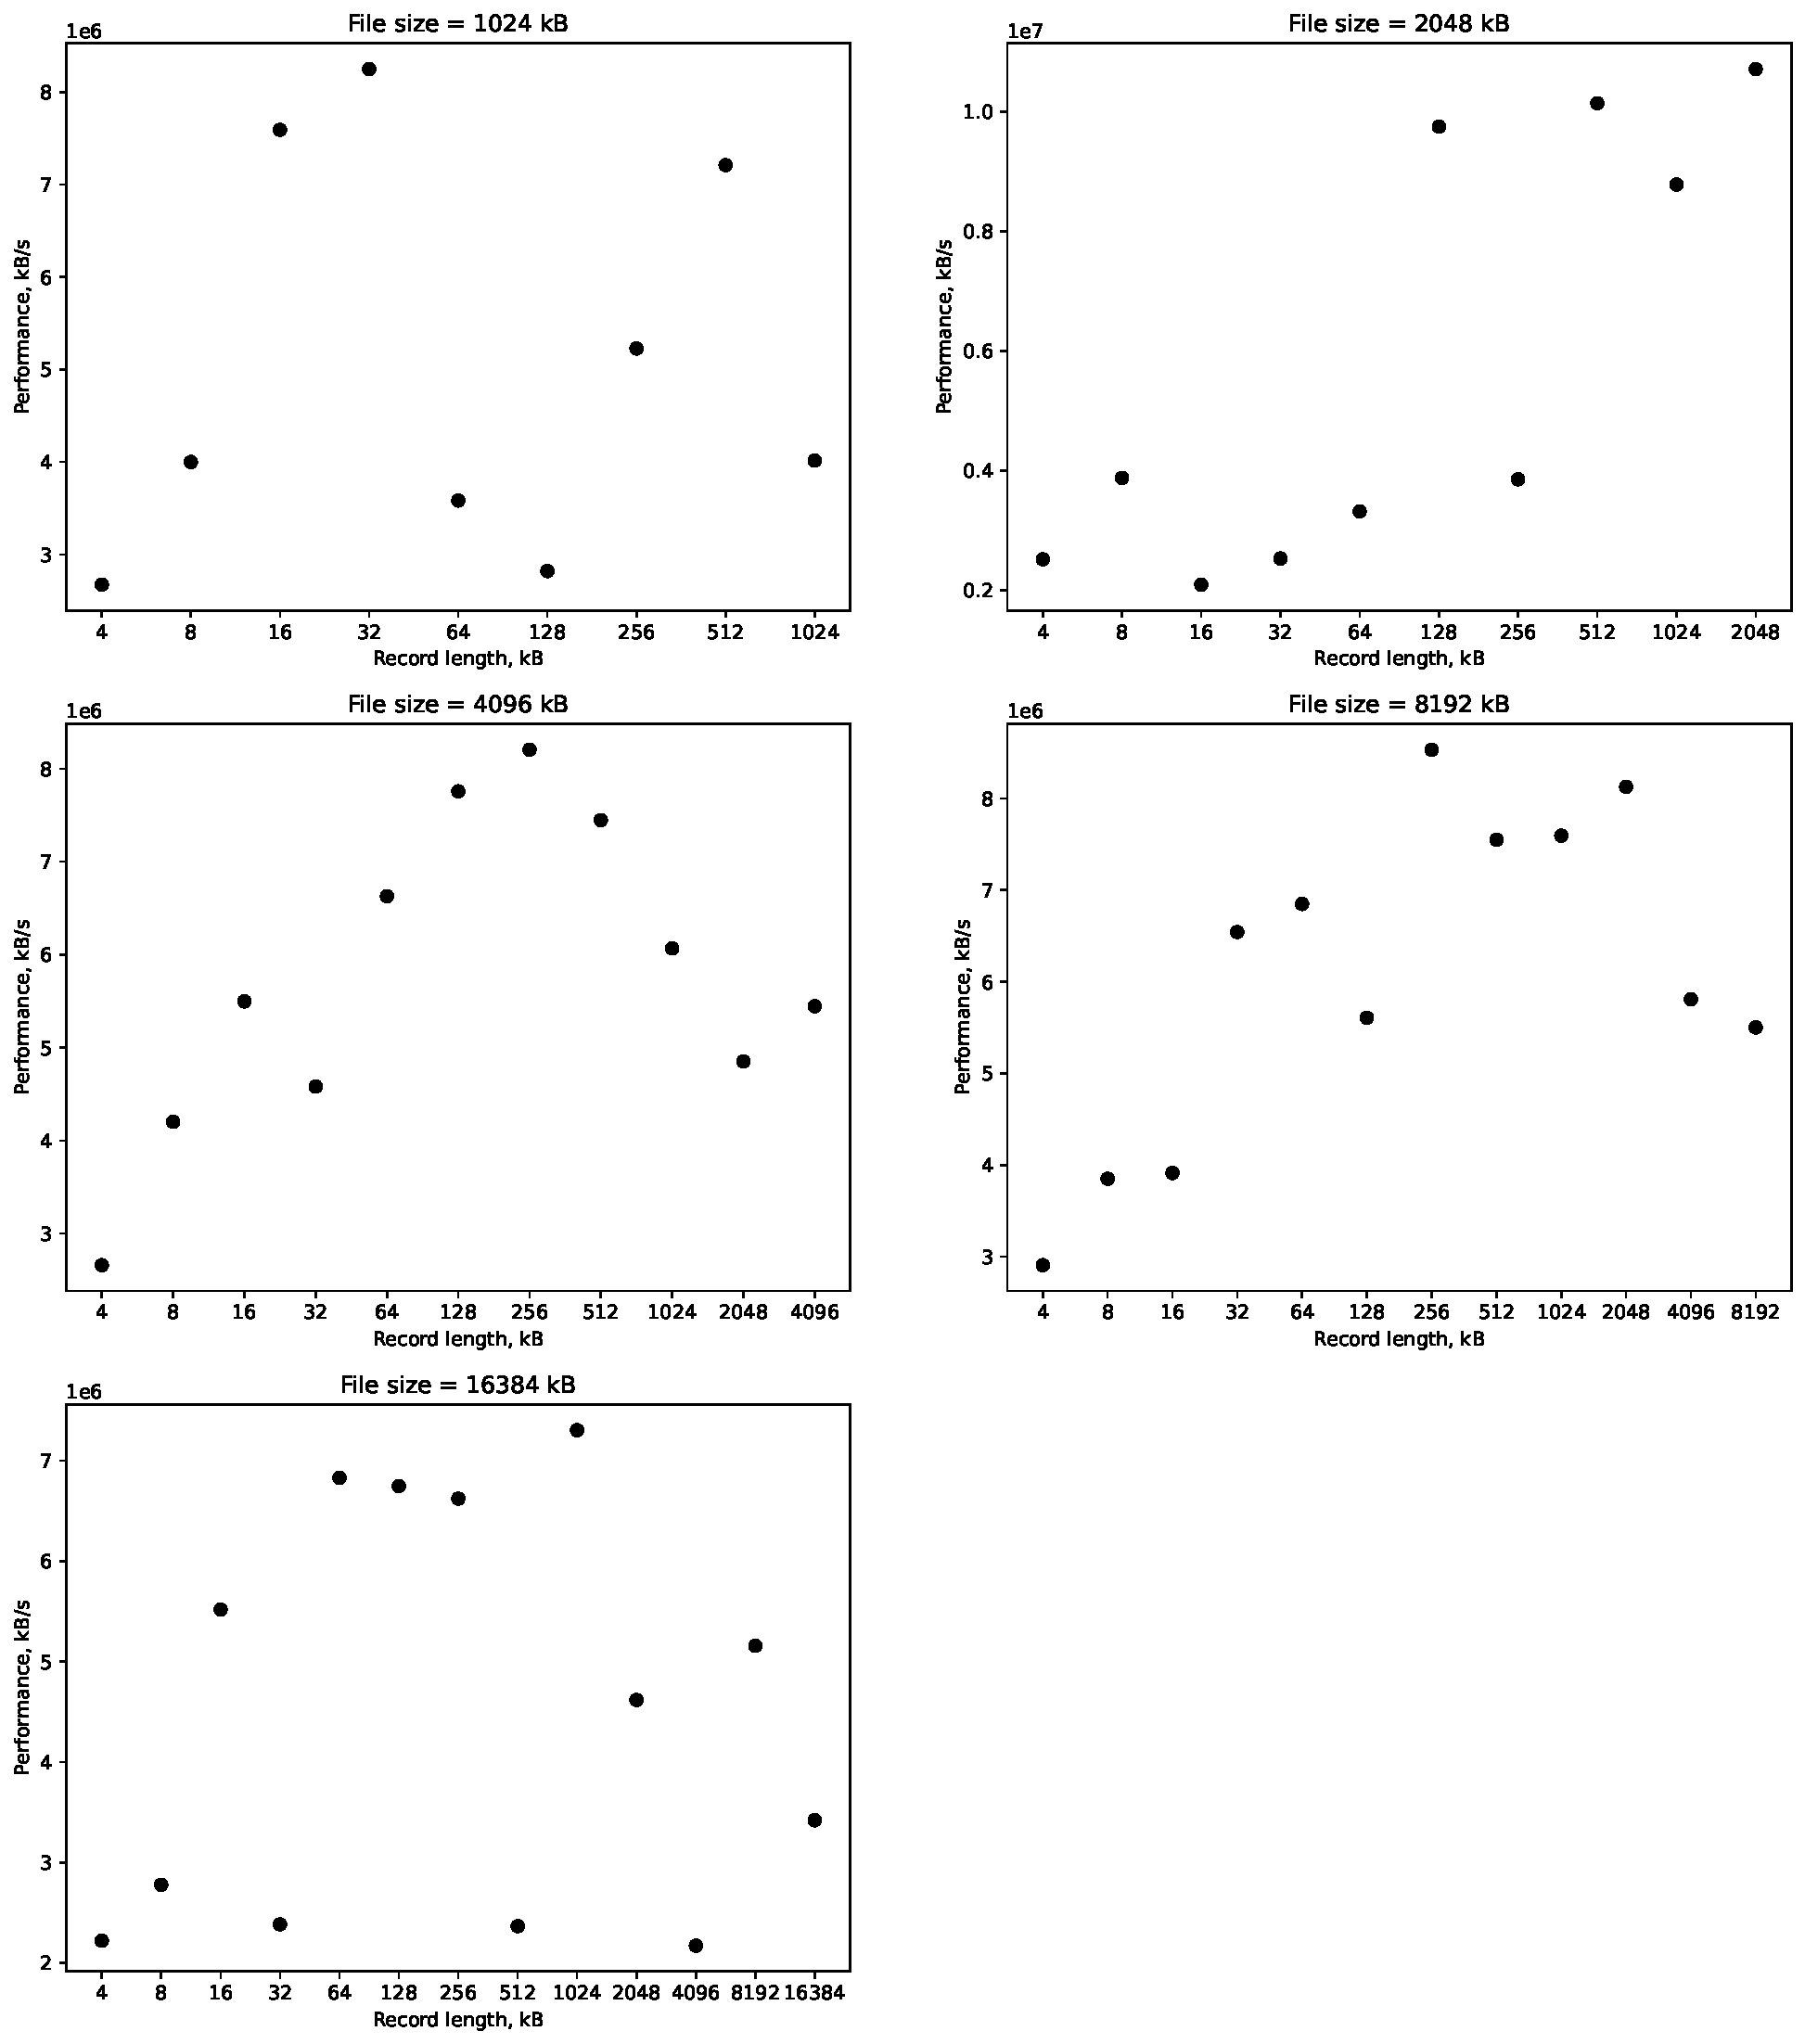
\includegraphics[width=1.0\textwidth]{figures/benchmarking/local/Re-Read.pdf}
	\end{center}
	\caption{IOZone output for \gls{APFS} \mbox{Re-Read}}
\end{figure}

\begin{figure}[!htb]
	\label{fig:bench_apfs_re_write}
	\begin{center}
		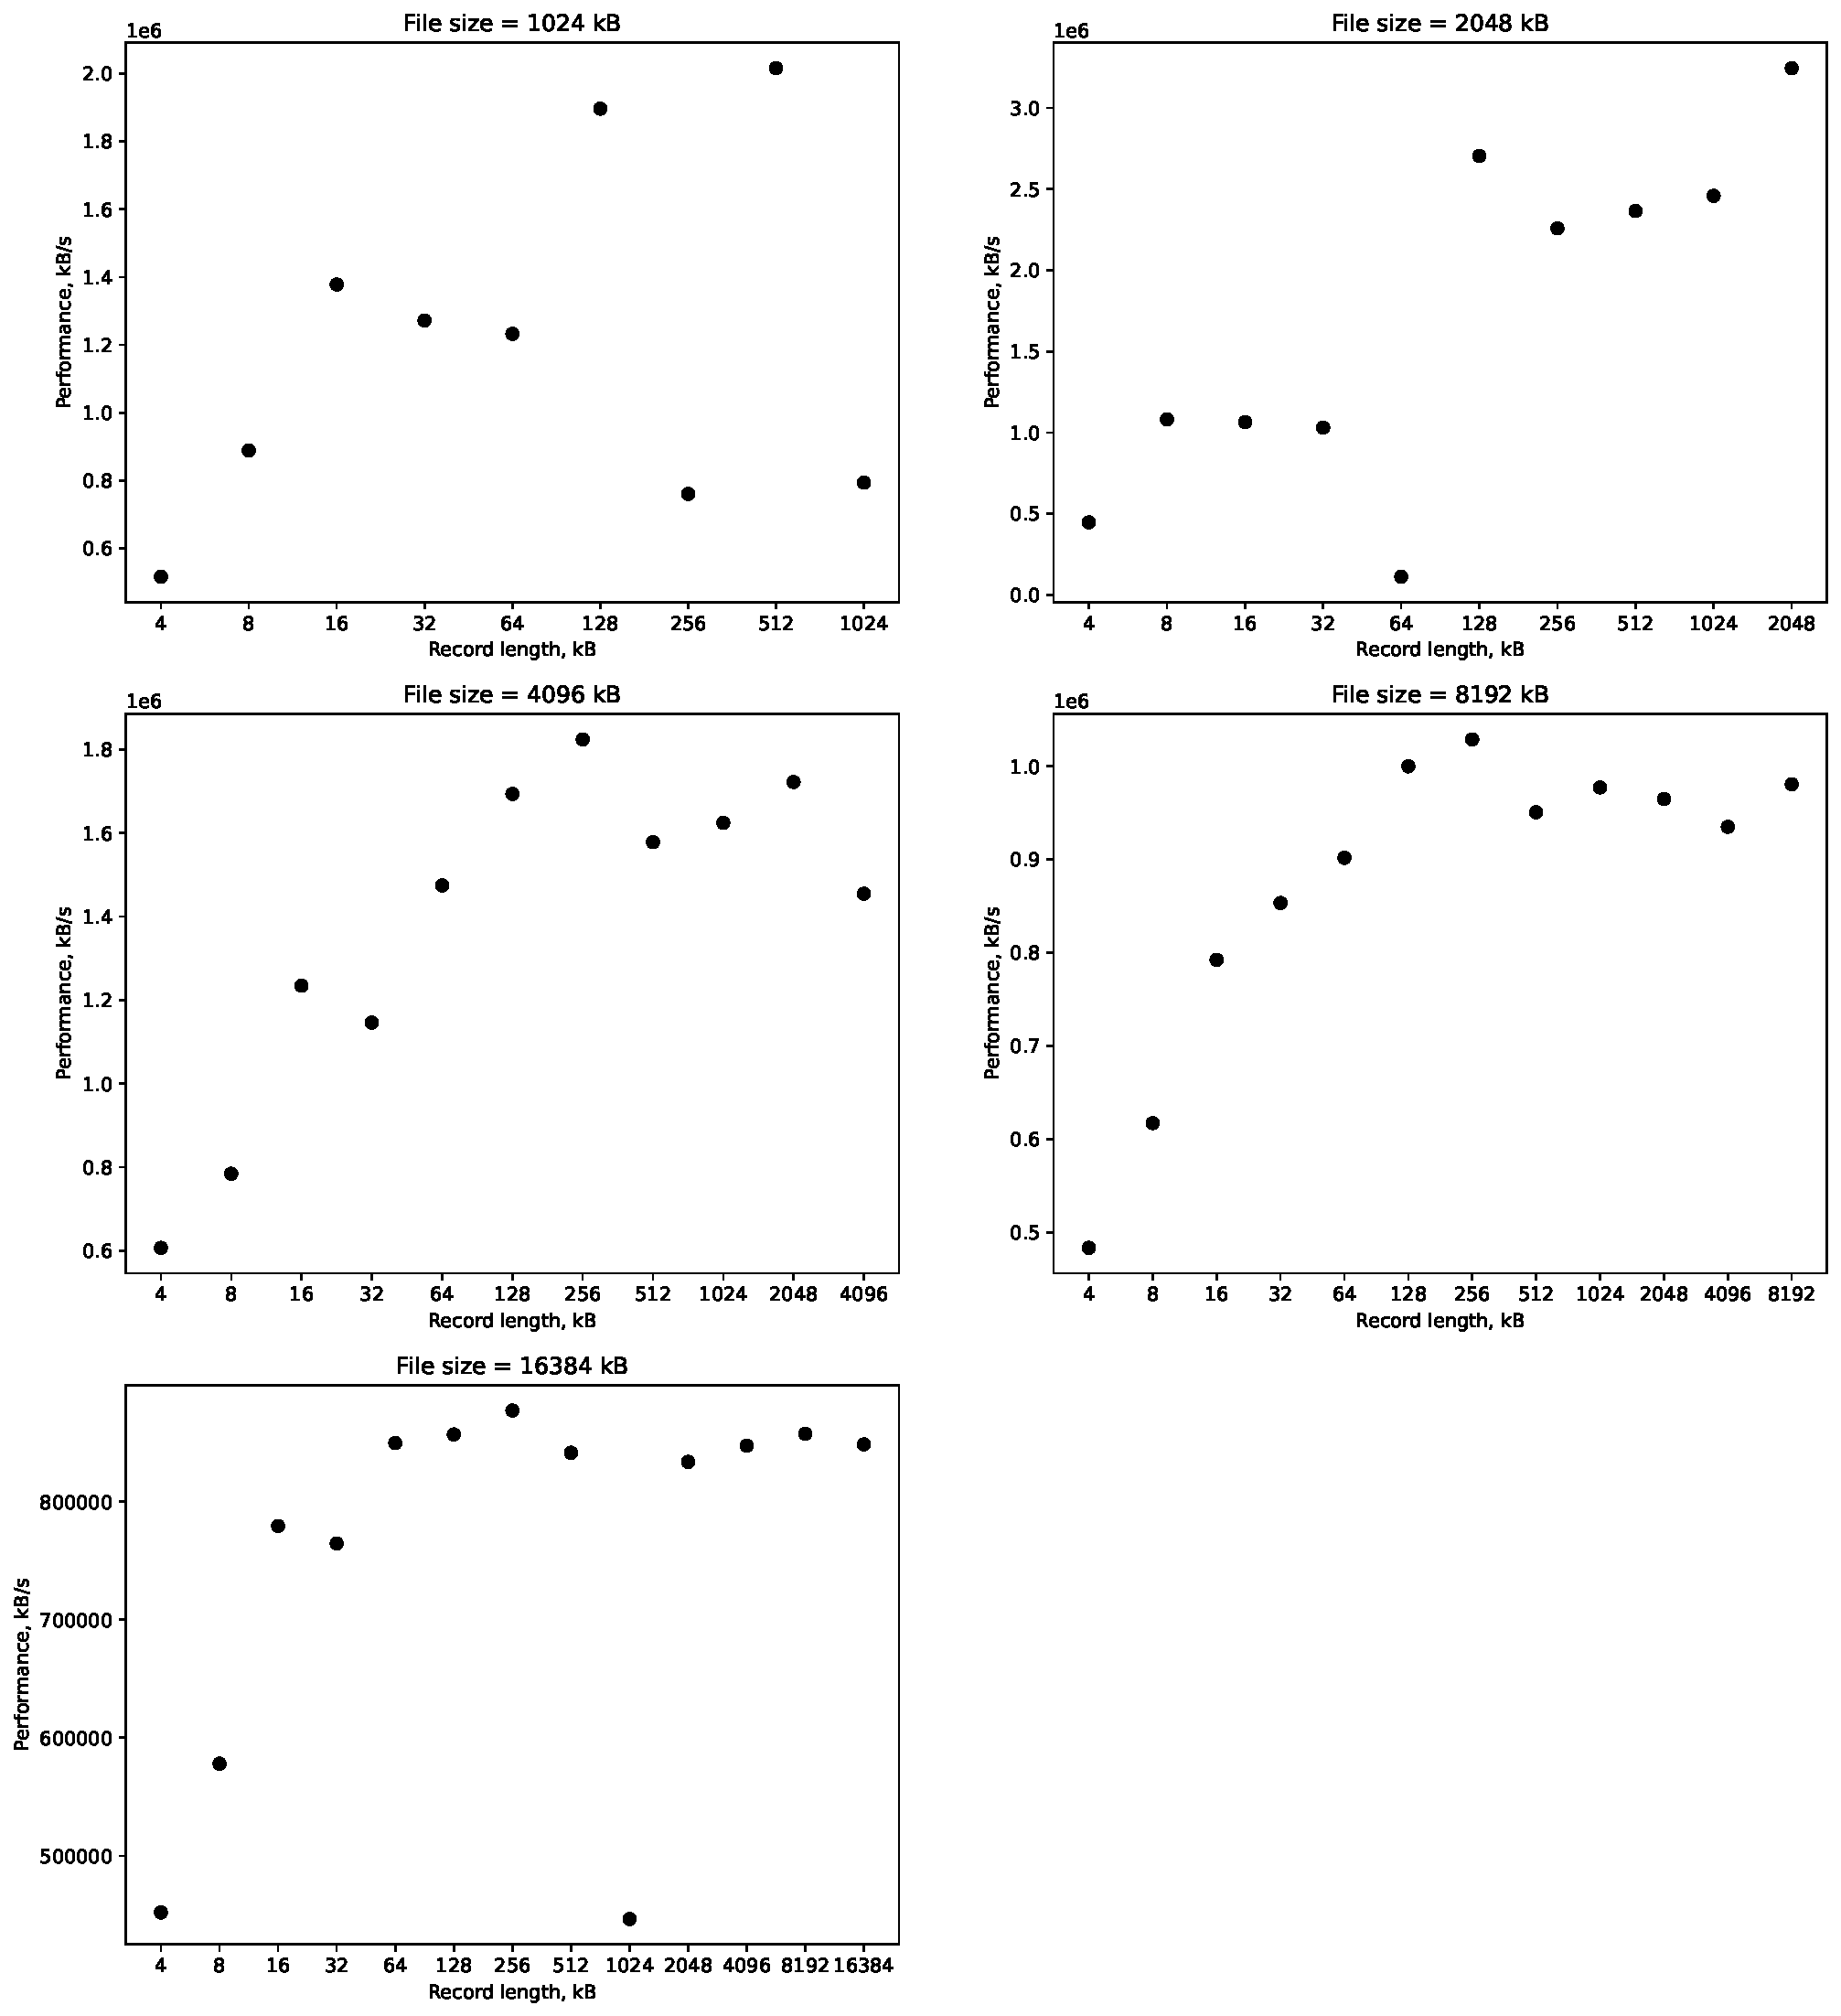
\includegraphics[width=1.0\textwidth]{figures/benchmarking/local/Re-Write.pdf}
	\end{center}
	\caption{IOZone output for \gls{APFS} \mbox{Re-Write}}
\end{figure}

\begin{figure}[!htb]
	\label{fig:bench_apfs_rnd_read}
	\begin{center}
		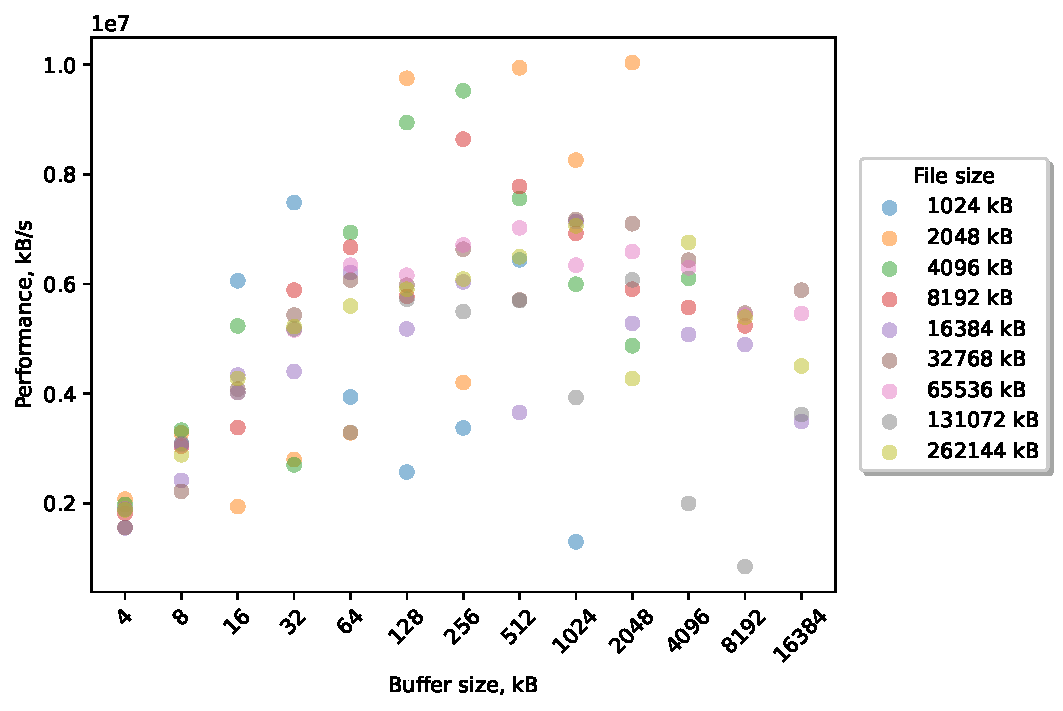
\includegraphics[width=1.0\textwidth]{figures/benchmarking/local/Random read.pdf}
	\end{center}
	\caption{IOZone output for \gls{APFS} Random read}
\end{figure}

\begin{figure}[!htb]
	\label{fig:bench_apfs_rnd_write}
	\begin{center}
		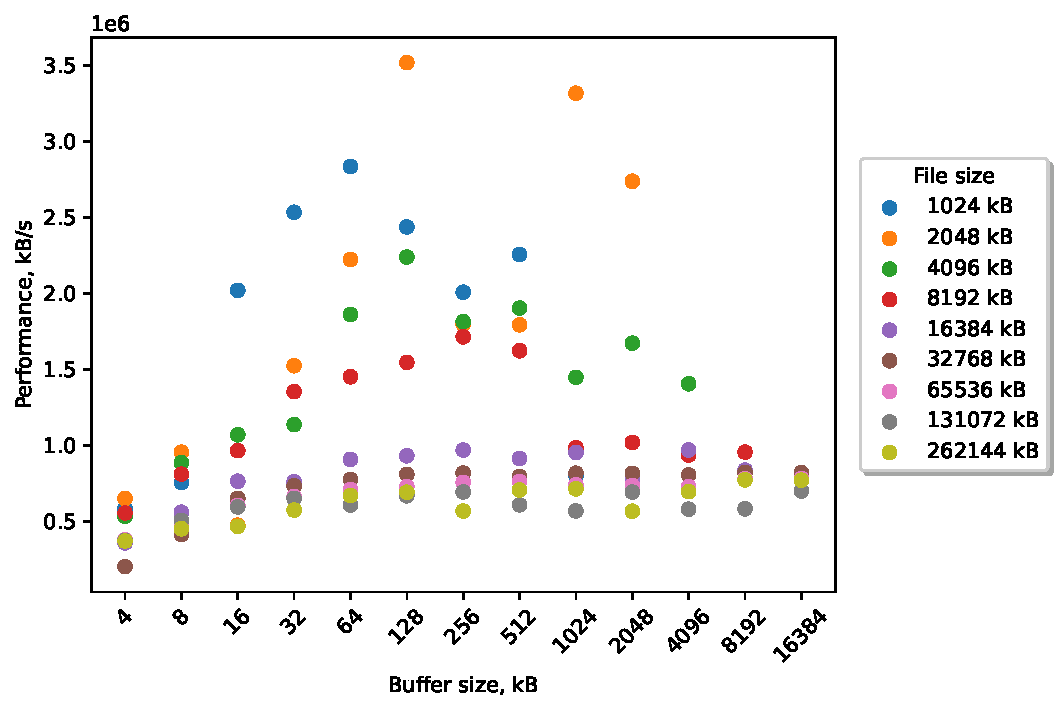
\includegraphics[width=1.0\textwidth]{figures/benchmarking/local/Random write.pdf}
	\end{center}
	\caption{IOZone output for \gls{APFS} Random write}
\end{figure}